% Page style for this chapter
	\pagestyle{fancy}
	\lhead{{\sffamily \MakeUppercase{2. The Peripheral Auditory System}}}
	\chead{}
	\rhead{{\sffamily \MakeUppercase\rightmark}}
	\lfoot{}
	\cfoot{{\sffamily \thepage}}
	\rfoot{}
	
\chapter{Anatomy and Physiology of the Peripheral Auditory System}

% Textbox
\begin{center}
	\begin{tcolorbox}[title=\boxtitle]
		\begin{itemize}[leftmargin=*,labelindent=2ex,labelsep=1.5ex,itemsep=0pt,parsep=0pt]
		    \item What structures are involved in hearing perception?
    		\item What does the cochlea look like?
			\item How does normal hearing work?
		\end{itemize}
	\end{tcolorbox}
\end{center}

%% ============================================================== Anatomy Review

\section{Anatomy Review}
\label{sect:anatomy_review}

\subsection{Overview of the Auditory Pathway}

The ability to hear involves a chain of anatomical structures that together form
the auditory pathway. It includes the various components of the ear, which are
responsible for the detection and encoding of sound stimuli, the neural pathways
that relay the encoded neural signal to the brain, and the auditory cortex, the
part of the brain that processes and interprets the received
signal~\cite{goldstein2009}.

The ear can be divided into three distinct regions: the external ear, the middle
ear, and the inner ear, as illustrated in Figure~\ref{fig:ear_overview}. Each
region is described briefly below.

\subsubsection{The External Ear}

The purpose of the external ear is to collect and direct sound waves towards the
middle ear. This is primarily facilitated by the \emph{auricle}, a cartilaginous
structure making up the portion of the ear visible from outside the body. Its
shape helps to funnel sound waves into the \emph{external acoustic meatus}, a
narrow tunnel that passes through the temporal bone of the skull. At the medial
end of the meatus is a thin sheet of connective tissue called the \emph{tympanic
membrane}, commonly known as the eardrum.

\begin{figure}[p]
	\centering
	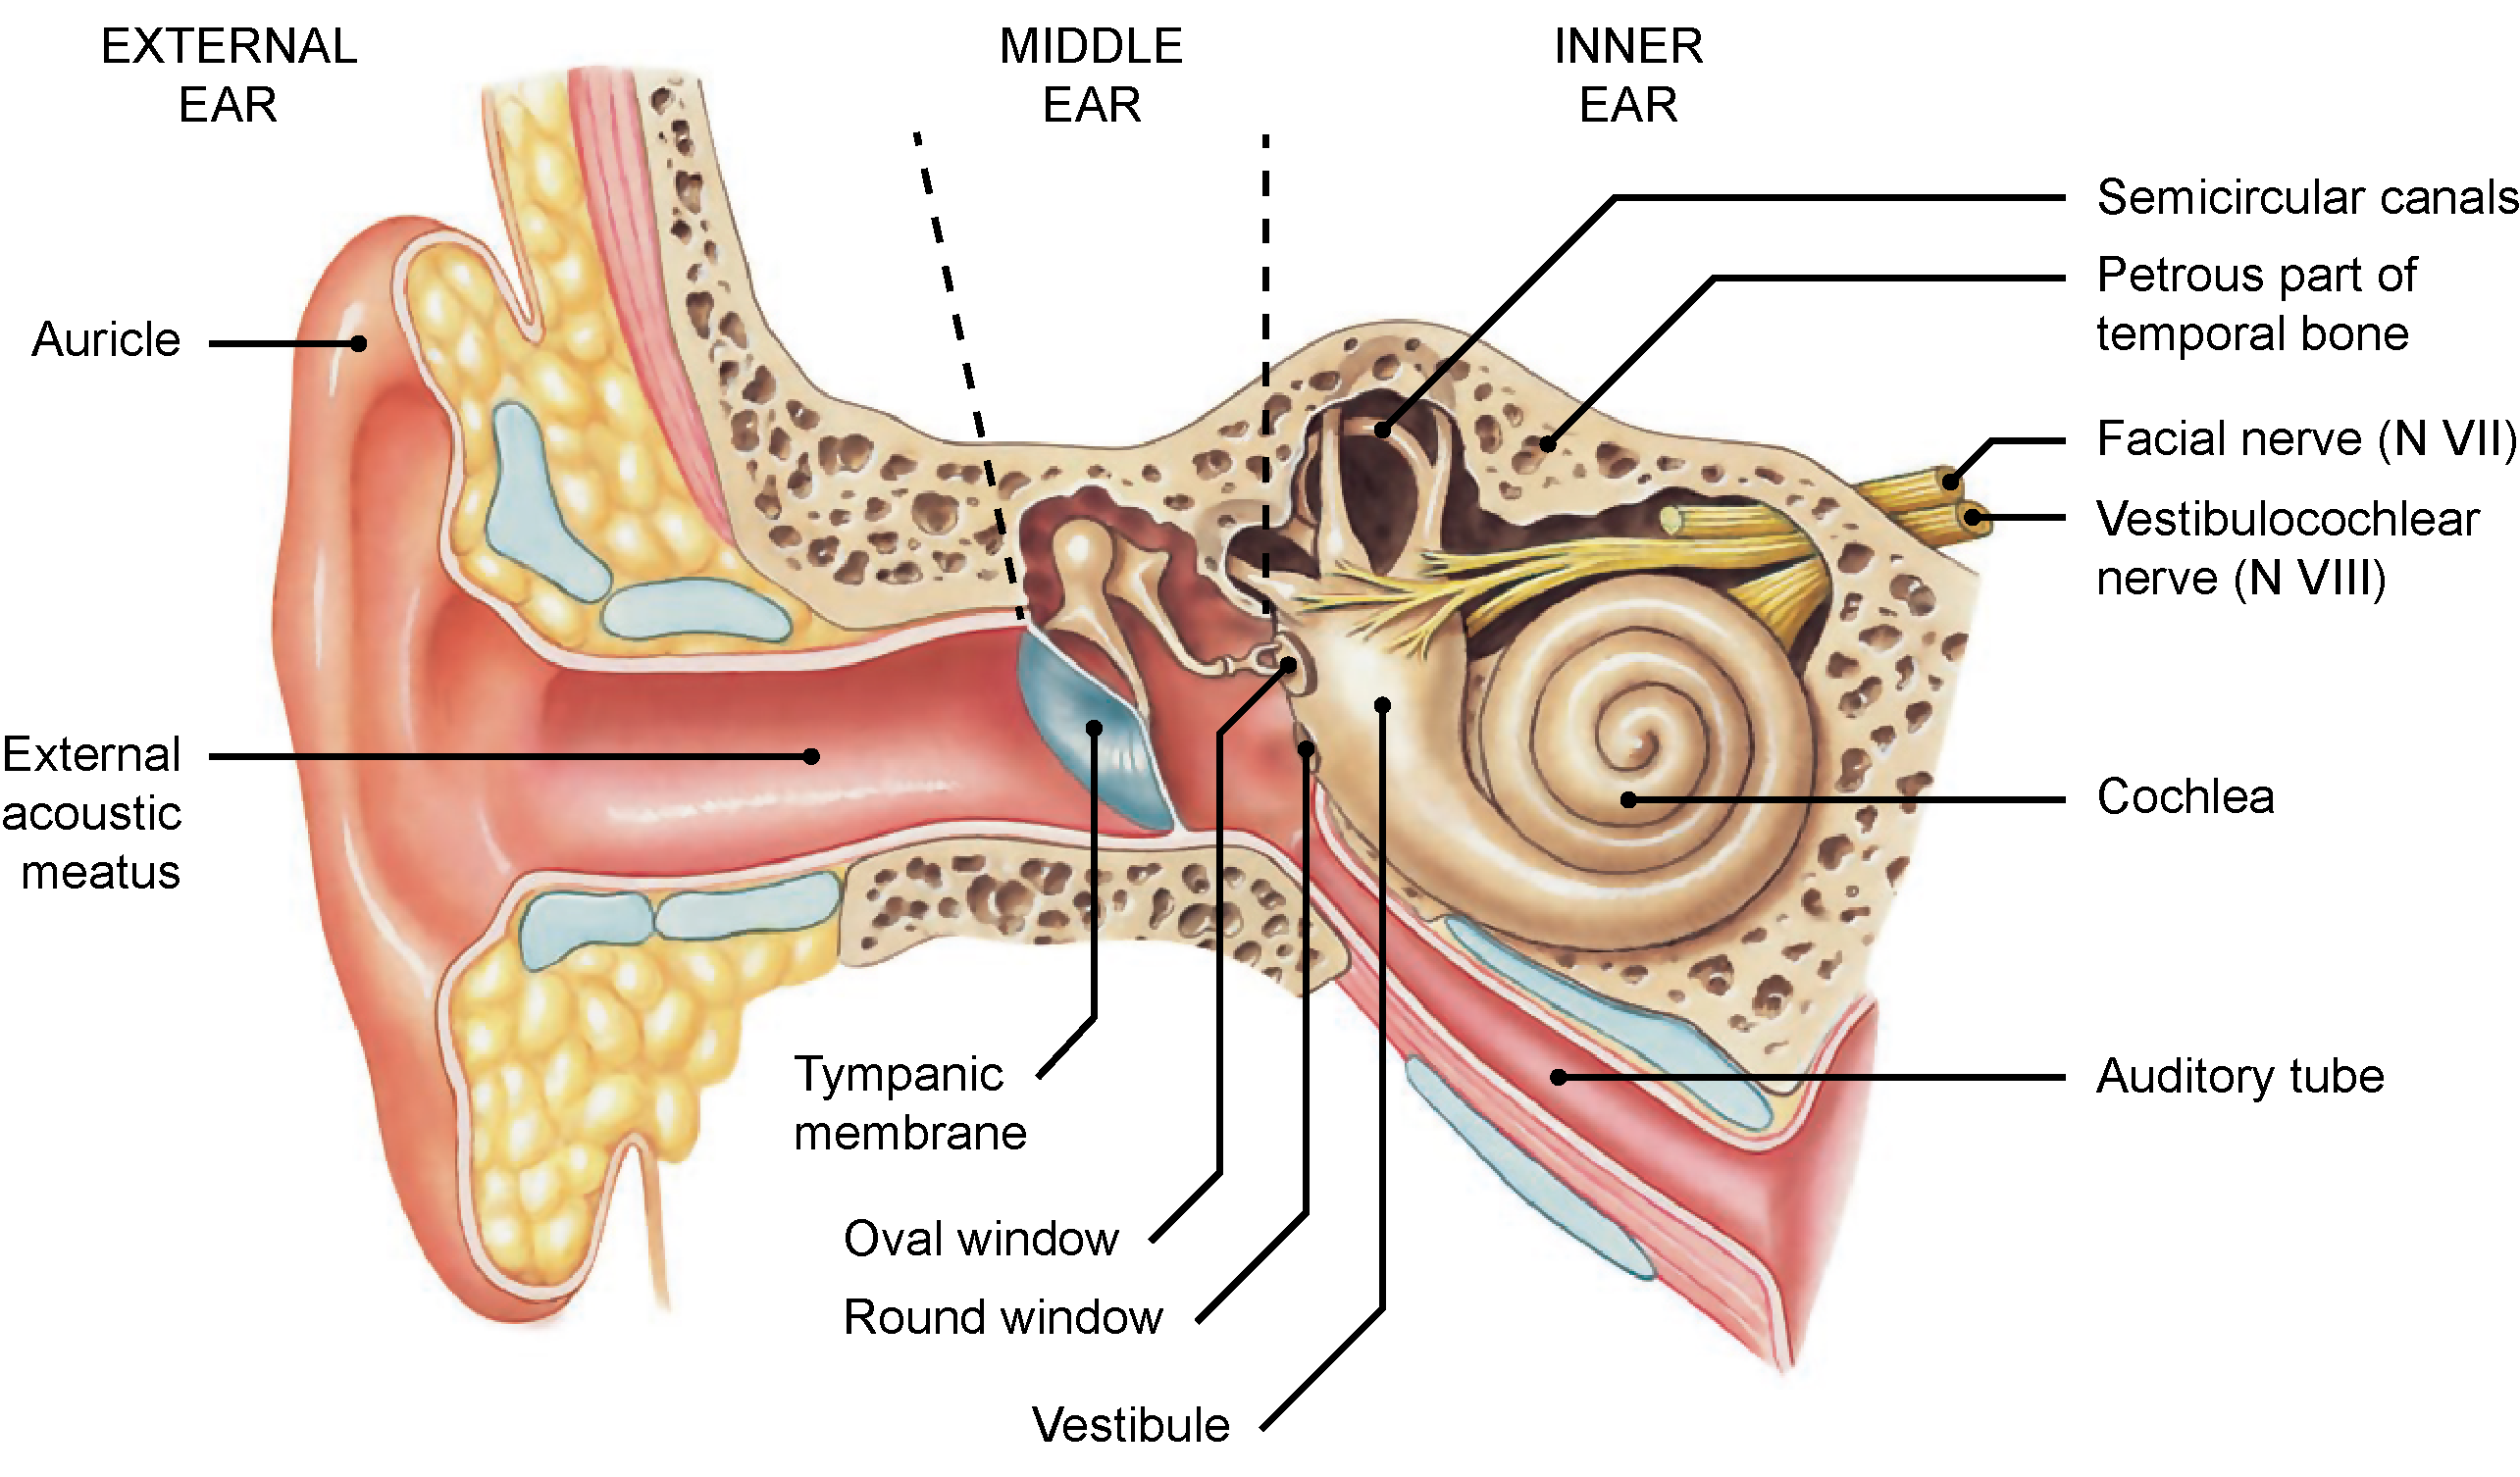
\includegraphics[width=\textwidth]{Background/ear_labelled.pdf}
	\caption[The anatomy of the ear]{The anatomy of the ear. (Image adapted from
	Martini~\etal~\cite{martini2006}. Copyright \textcopyright{} 2006, Daryl Fox.)}
	\label{fig:ear_overview}
\end{figure}

\begin{figure}[p]
	\centering
	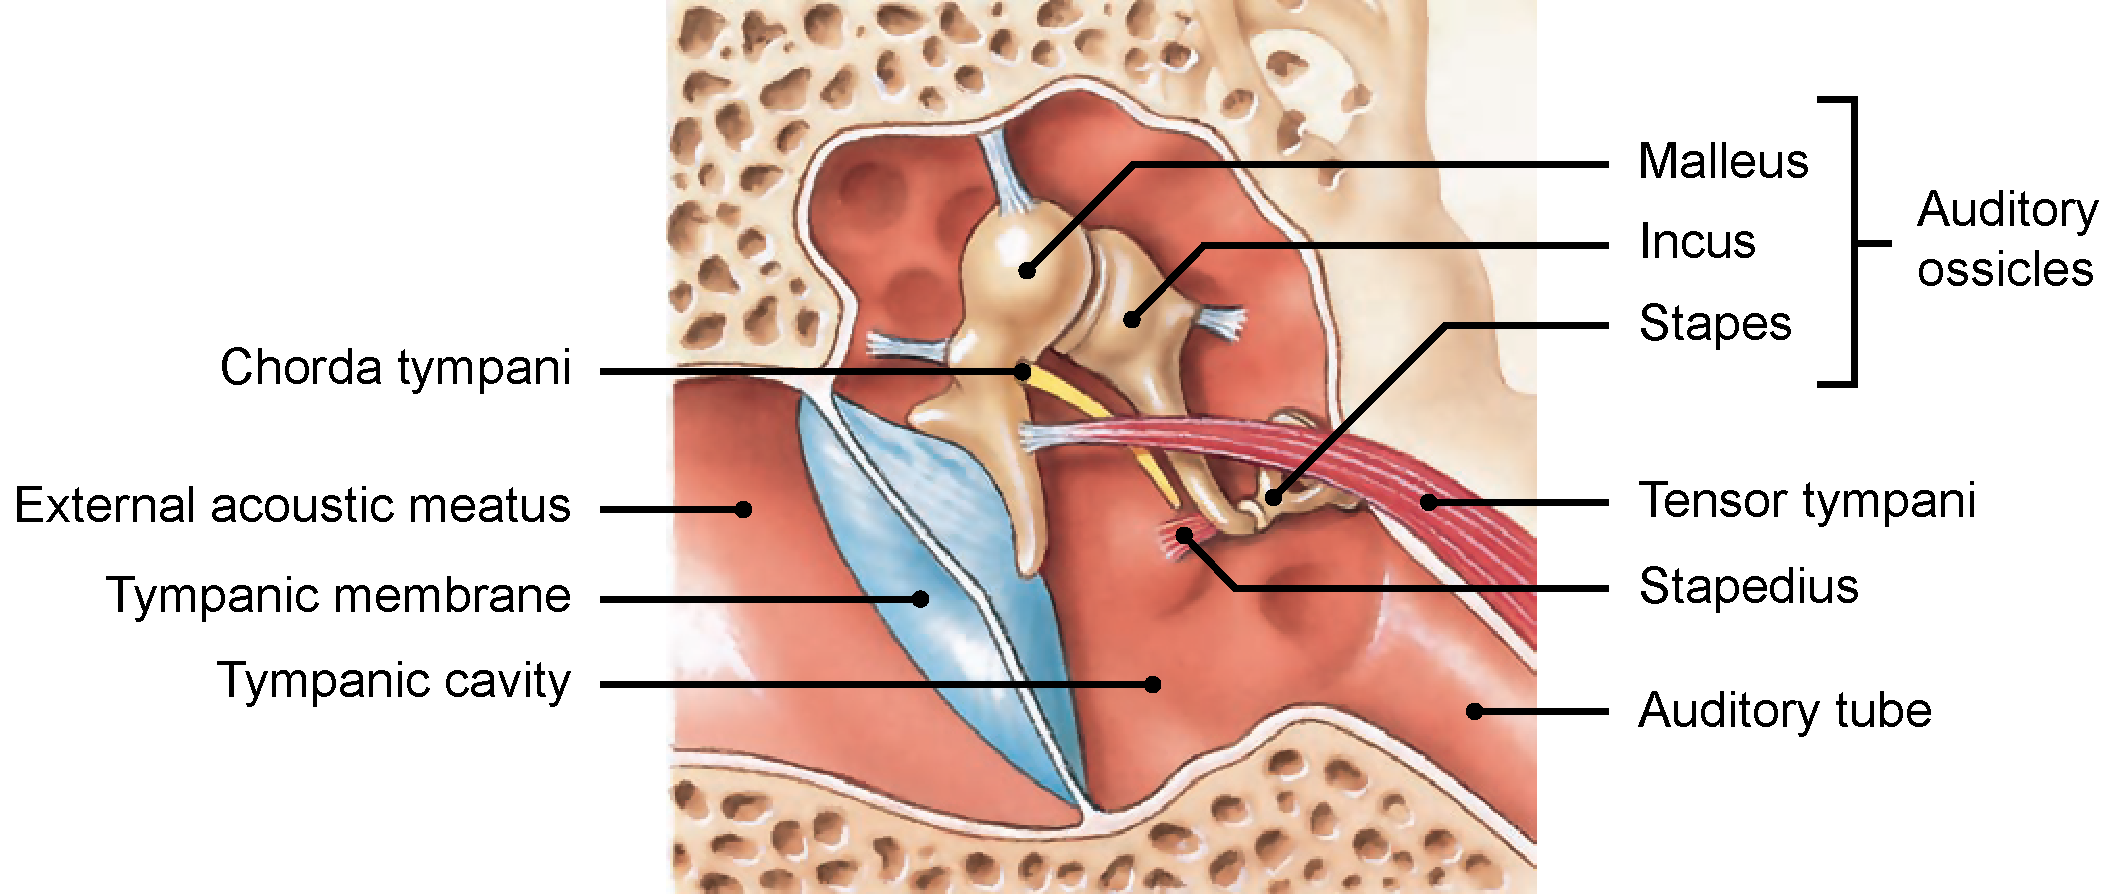
\includegraphics[width=13.3cm]{Background/middle_ear_labelled.pdf}
	\caption[Structures within the tympanic cavity]{Structures within the
	tympanic cavity. (Image adapted from Martini~\etal~\cite{martini2006}.
	Copyright \textcopyright{} 2006, Daryl Fox.)}
	\label{fig:middle_ear}
\end{figure}

\subsubsection{The Middle Ear}

On the other side of the tympanic membrane is a small, air-filled chamber called
the \emph{tympanic cavity} (see Figure~\ref{fig:middle_ear}). It opens
inferiorly into the \emph{auditory tube}, which leads to the nasopharynx. This
connection allows the air pressure on both the sides of the tympanic membrane to
be maintained at the external atmospheric pressure.

The key feature of the middle ear is its three tiny bones---the \emph{malleus},
the \emph{incus}, and the \emph{stapes}---collectively known as the
\emph{auditory ossicles}. The malleus is attached to the tympanic membrane
inferiorly and to the incus superiorly; in turn, the incus is linked to the
stapes, whose footplate is fused to an opening in the bony wall of the inner ear
known as the \emph{oval window} (see Figure~\ref{fig:ear_overview}). The
ossicles conduct and amplify the vibrations of incoming sound waves from the
tympanic membrane through the oval window to the inner ear.

Three other structures located in the middle ear are the \emph{tensor tympani}
and \emph{stapedius} muscles, and the \emph{chorda tympani} nerve. The muscles
prevent excessive movement of the tympanic membrane and ossicles that would
otherwise damage these delicate structures. The nerve carries taste sensations,
and passes through the tympanic cavity to join with the nearby \emph{facial
nerve} (or seventh cranial nerve, N~VII).

\subsubsection{The Inner Ear}

Sensory receptors for both hearing and equilibrium are housed in the chambers of
the inner ear (Figure~\ref{fig:inner_ear}). The \emph{membranous labyrinth},
which contains a fluid called \emph{endolymph}, is surrounded by the \emph{bony
labyrinth} (also known as the \emph{otic capsule}~\cite[p. 62]{jahn2001}), and
the space between them is filled with another fluid called \emph{perilymph}.
Endolymph and perilymph are both extracellular fluids but they have different
compositions, as shown in Table~\ref{table:fluid_composition}. The high
potassium concentration of endolymph is required for normal hearing function and makes it
unique amongst bodily fluids. The composition of perilymph is similar to that of
cerebrospinal fluid (CSF), likely because they are joined via the
\emph{perilymphatic duct}. There are subtle variations in composition between
the two perilymphatic fluid chambers, with only the amount of protein showing a
large discrepancy.

\begin{figure}
	\centering
	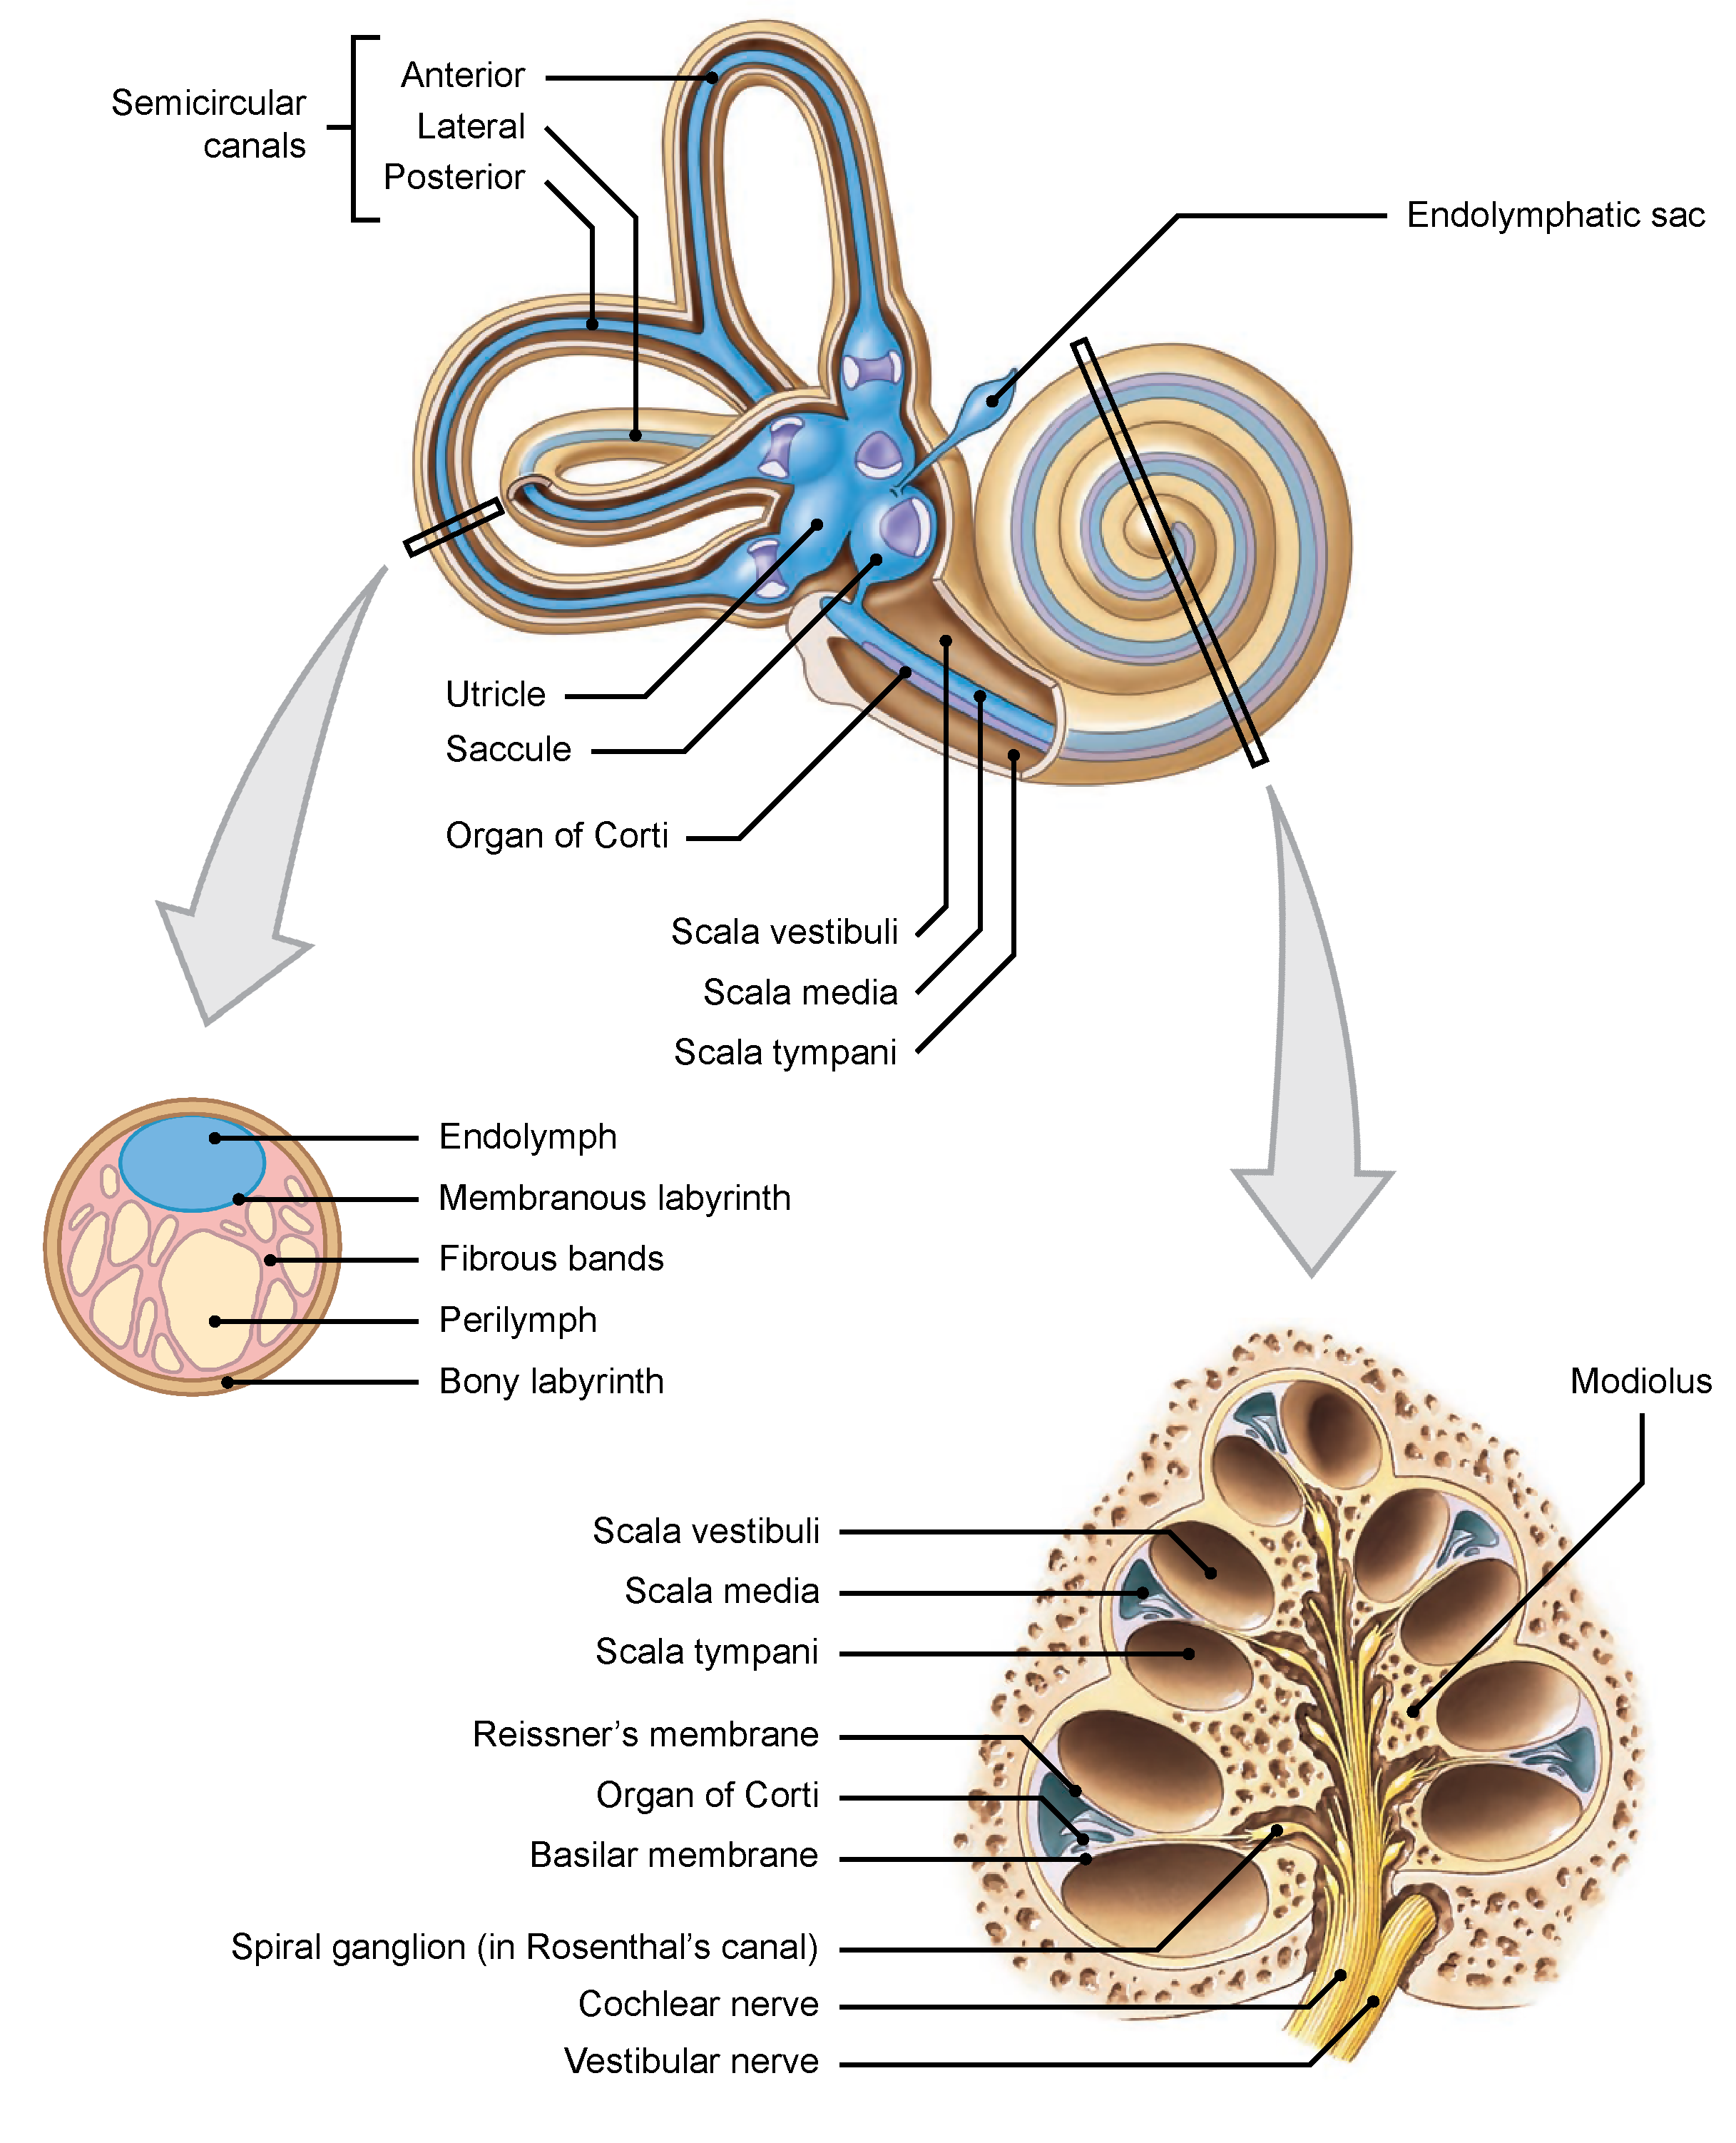
\includegraphics[width=\textwidth]{Background/labyrinths_labelled_ext.pdf}
	\caption[Labyrinths of the inner ear]{Labyrinths of the inner ear. (Image
	adapted from Martini~\etal~\cite{martini2006}. Copyright \textcopyright{} 2006,
	Daryl Fox.)}
	\label{fig:inner_ear}
\end{figure}

\begin{table}
	\centering
	\sffamily
	\small
	\caption[Composition of the inner ear fluids]{Composition of the inner ear
	fluids. All values are reported in millimolar (mM), except for protein.
	Measurements were obtained from various studies on guinea pigs and rodents. Not
	all constituents have been listed. (Data from Wangemann and
	Schacht~\cite{wangemann1996}.)}
	\label{table:fluid_composition}
	
	\begin{tabular}{l c c c c}
		\toprule
		\textbf{Component}	& \textbf{Endolymph of}	& \textbf{Perilymph of}	
			& \textbf{Perilymph of}		& \textbf{Cerebrospinal} \\
							& \textbf{scala media}	& \textbf{scala vestibuli}
			& \textbf{scala tympani}	& \textbf{fluid} \\
		\midrule
		
		\csvreader[late after line=\\]%
			{Background/fluid_compositions.csv}%
			{Component=\comp,Endolymph (SM)=\esm,Perilymph (SV)=\psv,Perilymph (ST)=\pst,CSF=\csf}%
 			{\comp & \esm & \psv & \pst & \csf}%
		\bottomrule
	\end{tabular}
	
\end{table}

The posterolateral aspects of the inner ear, namely the \emph{vestibule} (see
Figure~\ref{fig:ear_overview}) and the semicircular canals, together form the
\emph{vestibular complex}. Sensations of gravity, linear acceleration and head
rotation all arise from the receptors in this region. The sensation of hearing
occurs in the anteromedial aspect, which is named the \emph{cochlea} after its
distinctive snail shell appearance. For both of these senses, the reception of
stimuli and their transduction into neuronal signals is handled by highly
specialised mechanoreceptors called \emph{hair cells} (see inset,
Figure~\ref{fig:corti}).

The structure of the cochlea is described in more depth in
\S\ref{section:cochlea_detail}.

\subsubsection{Neural Pathways to the Auditory Cortex}
\label{section:neural_pathways}

Hair cells are monitored by the peripheral nerve endings of auditory neurons.
The cell bodies of these predominantly bipolar neurons are unmyelinated in
humans~\cite{ota1980} and are clustered together in the \emph{spiral ganglion},
housed within \emph{Rosenthal's canal} (see Figure~\ref{fig:inner_ear}). Their
myelinated axons combine to form the \emph{cochlear nerve}, which exits the
cochlea via its basal end and joins with the \emph{vestibular nerve} exiting the
vestibular complex to become the \emph{vestibulocochlear nerve}, also known as
the auditory nerve (or eighth cranial nerve, N~VIII). These branches, shown in
Figure~\ref{fig:tonotopy}, follow the \emph{internal auditory meatus} through
the petrous part of the temporal bone and are encased in CSF.

\begin{figure}
	\centering
	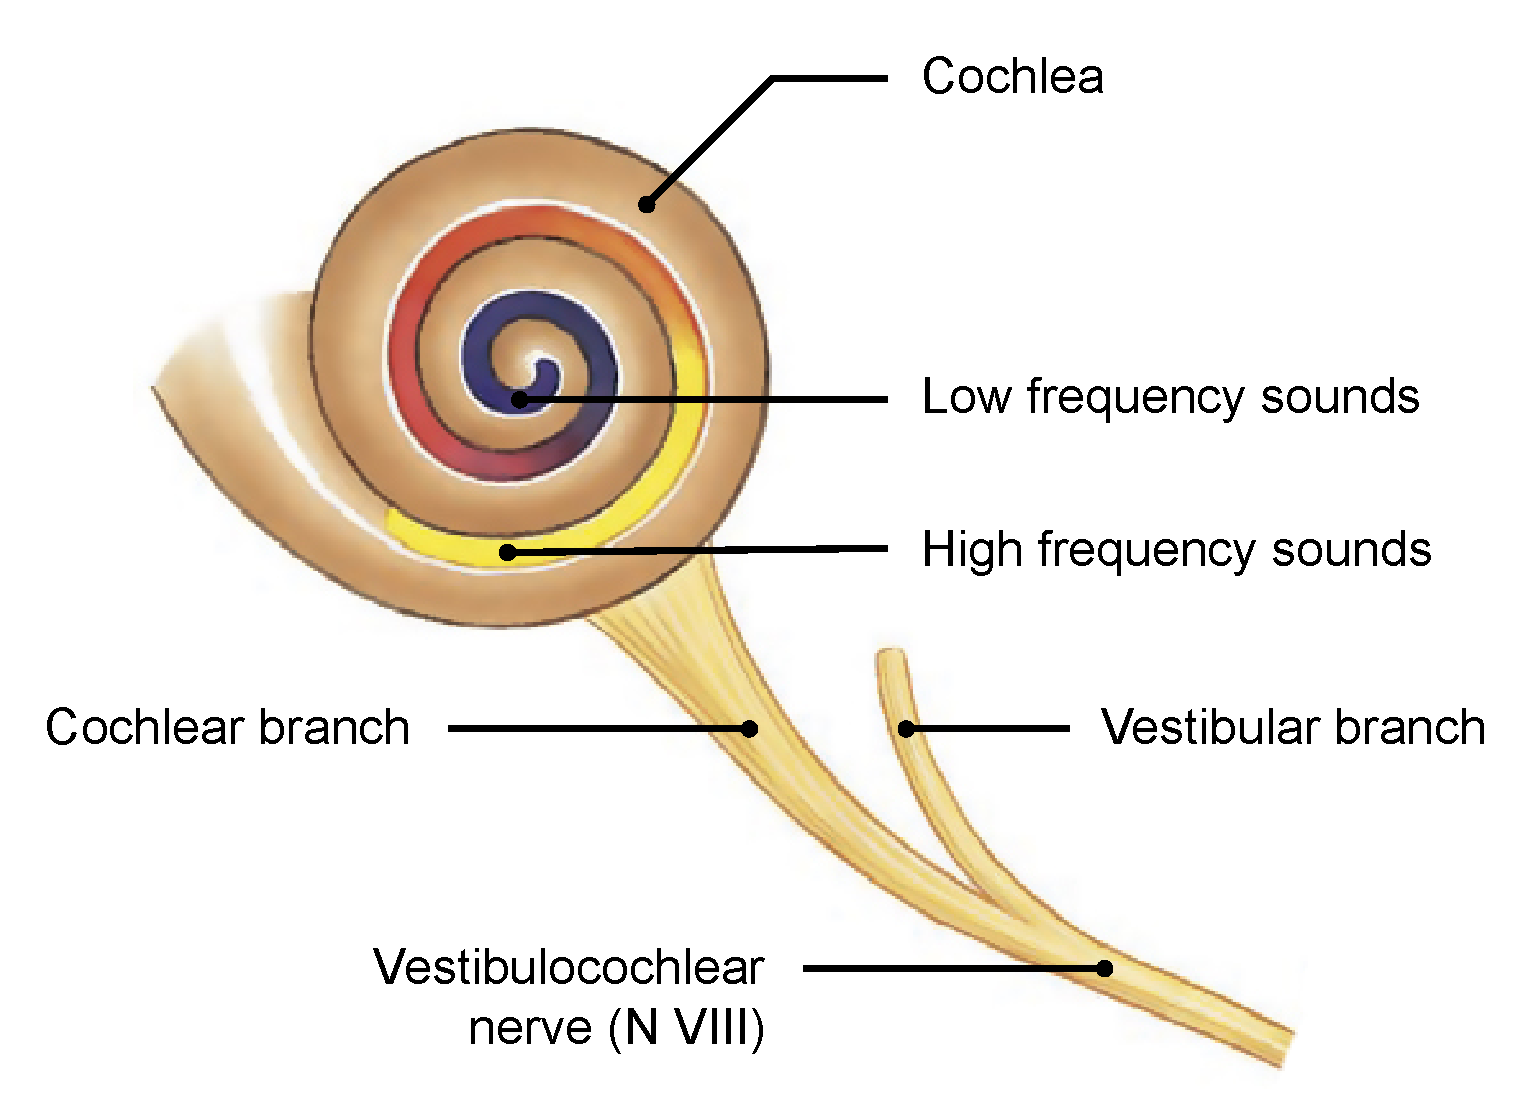
\includegraphics[width=9.8cm]{Background/tonotopy}
	\caption[Tonotopic organisation of the cochlea]{Tonotopic organisation of the
	cochlea. Low and high frequency receptors join together to form the cochlear
	branch of N VIII. The sequential frequency mapping is preserved and
	transferred to the auditory cortex (cf. Figure~\ref{fig:auditory_cortex}).
	(Image adapted from Martini~\etal~\cite{martini2006}. Copyright
	\textcopyright{} 2006, Daryl Fox.)}
	\label{fig:tonotopy}
\end{figure}

Upon reaching the ipsilateral \emph{cochlear nucleus} in the medulla oblongata,
second-order neurons decussate and ascend to the \emph{inferior colliculus},
which is responsible for auditory reflexes. Connecting neurons propagate the
signal to the \emph{medial geniculate nucleus} in the thalamus, before finally
reaching the \emph{auditory cortex} in the temporal lobe of the brain. These
pathways are illustrated in Figure~\ref{fig:auditory_cortex}.

\begin{figure}
	\centering
	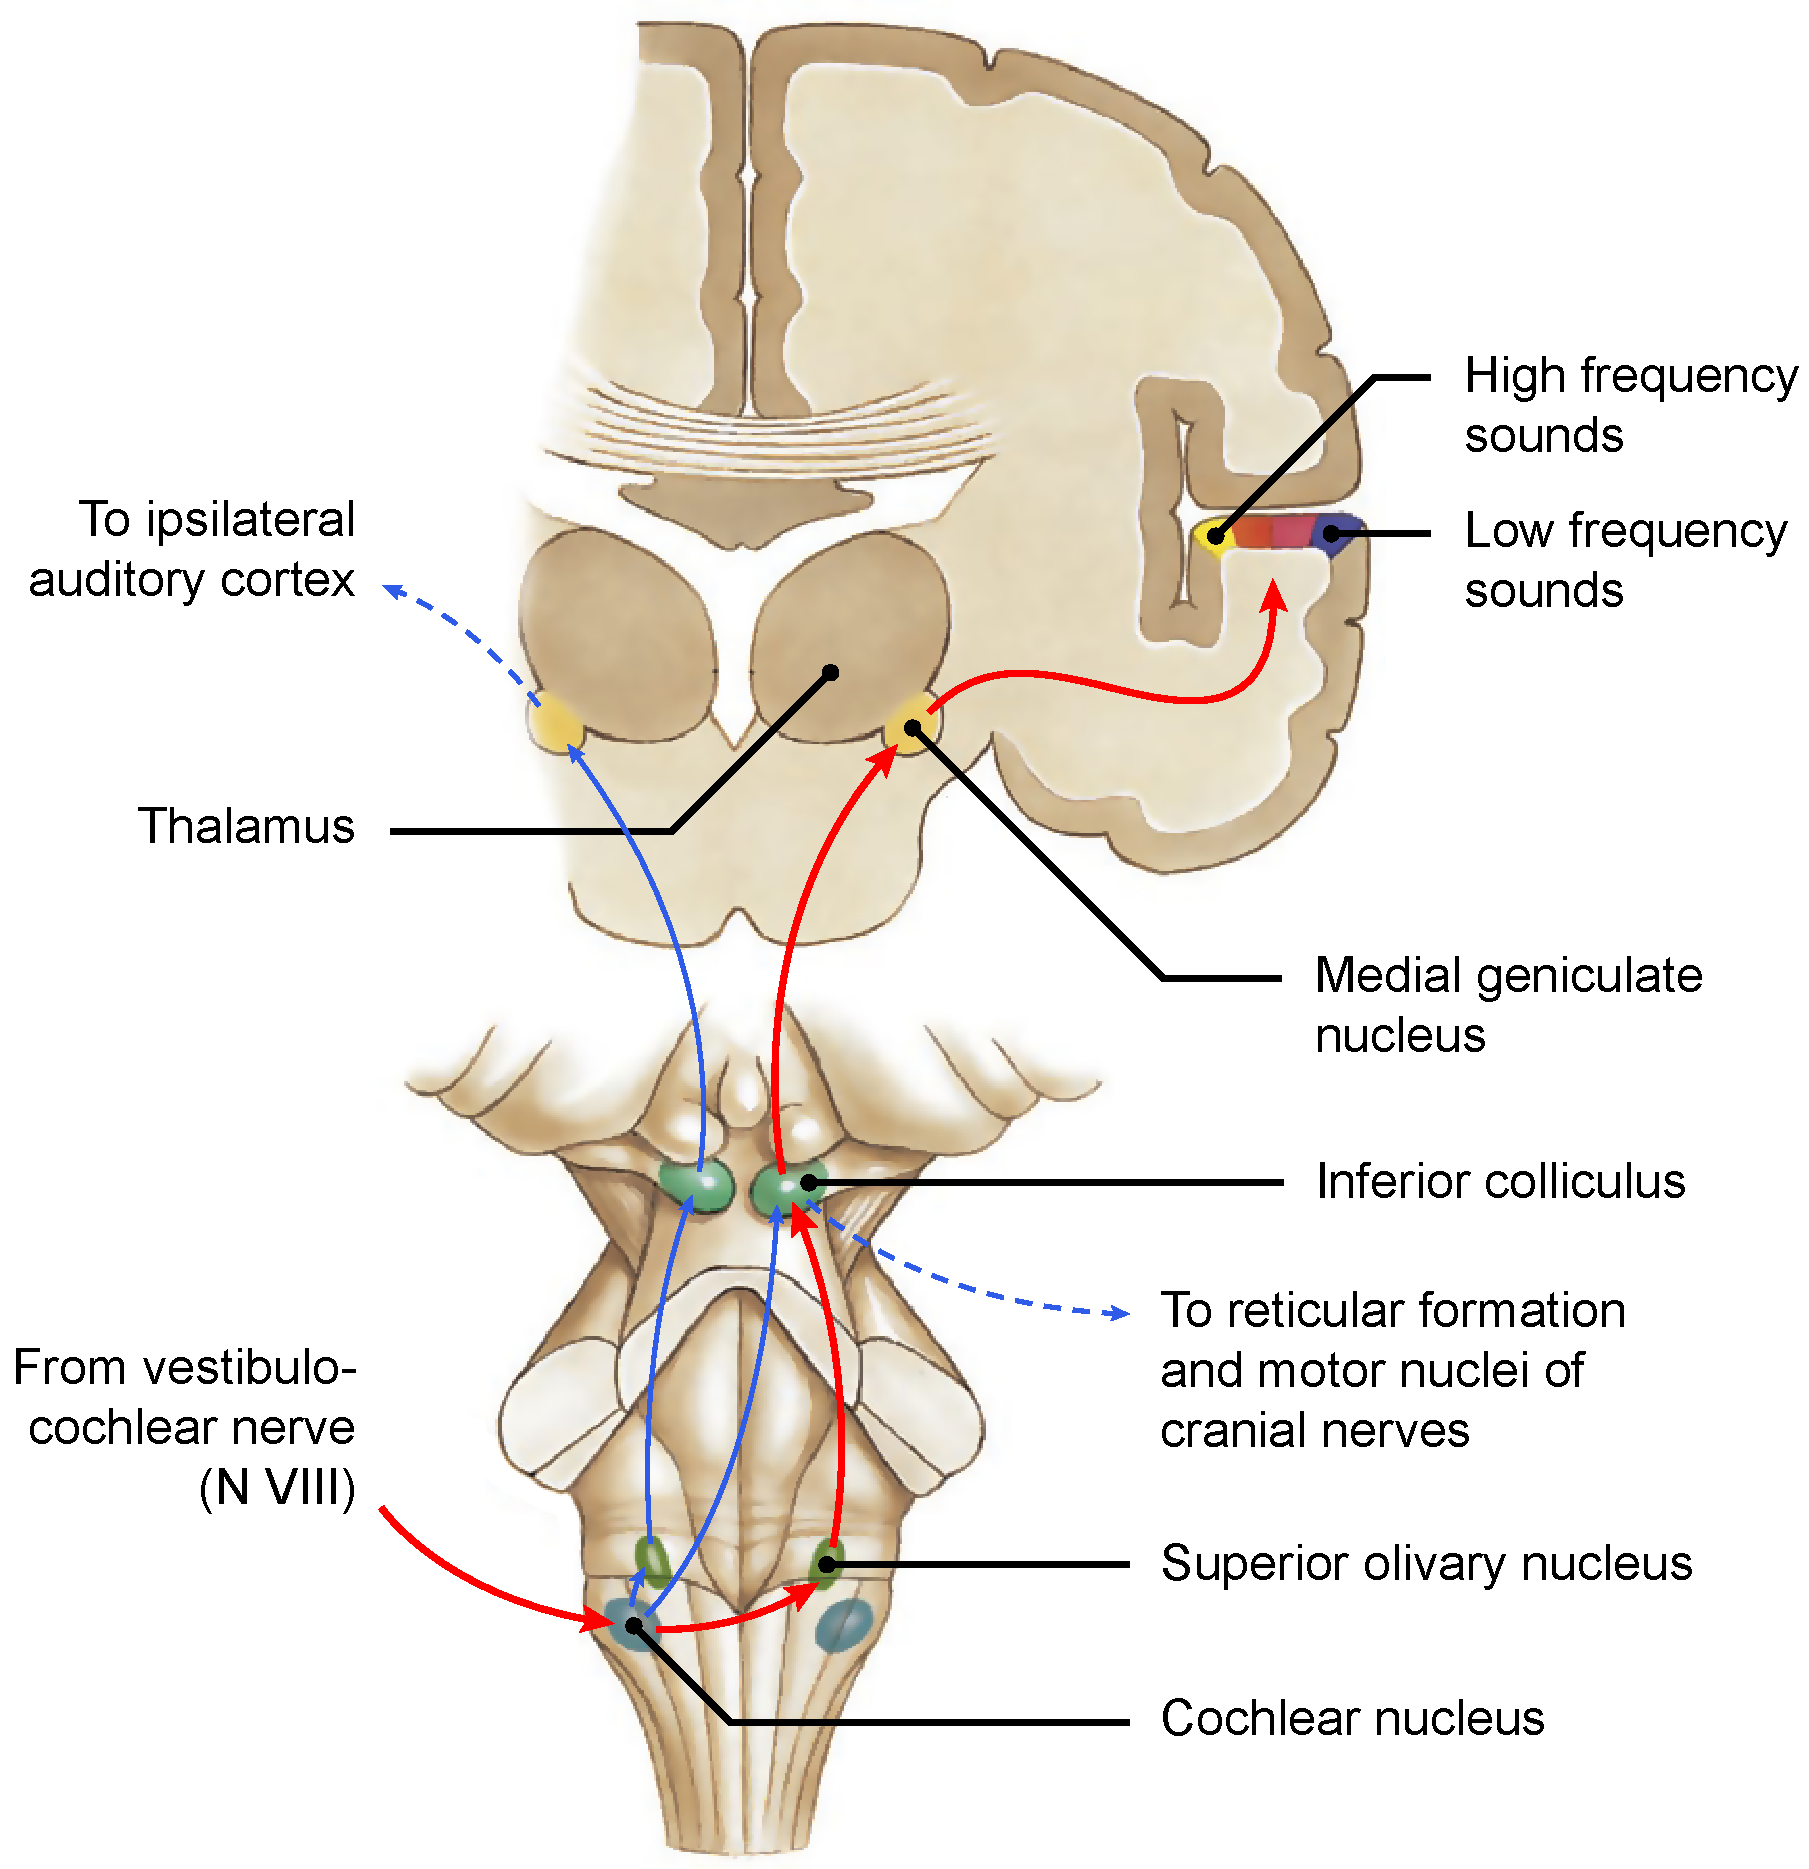
\includegraphics[width=12cm]{Background/cortex_labelled.pdf}
	\caption[Neural pathways to the auditory cortex]{Neural pathways to the
	auditory cortex. The primary pathway is shown by the red arrows, while
	secondary connections are marked by the blue arrows. The low and high
	frequency regions of the auditory cortex are arranged sequentially, analogous
	to the tonotopic organisation of the cochlea (cf. Figure~\ref{fig:tonotopy}).
	(Image adapted from Martini~\etal~\cite{martini2006}. Copyright
	\textcopyright{} 2006, Daryl Fox.)}
	\label{fig:auditory_cortex}
\end{figure}

% ============================================================= Cochlear anatomy

\subsection{Detailed Structure of the Cochlea}
\label{section:cochlea_detail}

The cochlea is a biological electromechanical system with three main classes of
internal structures: fluid spaces and structural support, sensory neuroanatomy,
and vasculature. Each of these is comprised of different tissue types and plays
a unique but interdependent role in the hearing process.

\subsubsection{Directional Terms}

Due to its tapered spiral shape, directions in the cochlea are usually described
relative to the \emph{mid-modiolar axis}, i.e. the axis through the centre of
the cochlea around which the labyrinths spiral (see
Figure~\ref{fig:directions}). There is also a consensus cochlear coordinate
system for quantitative measurements~\cite{verbist2010}. The key terms used in
this thesis are listed below:

\begin{description}
	\item[\textsf{Apical---Basal}] Any axis parallel to the mid-modiolar axis.
	\item[\textsf{Above---Below}] Towards the apex/base of the cochlea. Used when
	describing structures in a localised region.
	\item[\textsf{Radial}] Any axis perpendicular to the mid-modiolar axis.
	\item[\textsf{Medial---Lateral, or Central---Peripheral}] Towards/away from the
	mid-modiolar axis along a radial axis. The former pair is usually used in the
	context of a cross-sectional slice, while the latter pair is used in reference
	to the three-dimensional (3D) structure.
	\item[\textsf{Spiral}] The helical path followed by the labyrinths around the
	mid-modiolar axis.
	\item[\textsf{Turn}] A 360 degree segment of the cochlear spiral.
\end{description}

\begin{figure}
	\centering
	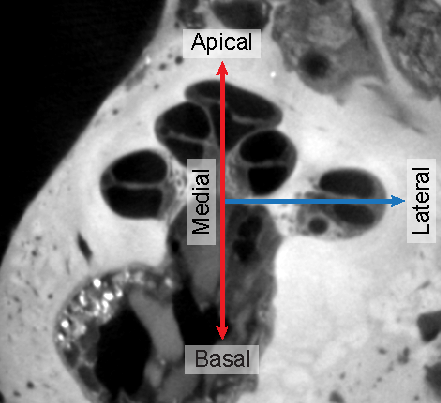
\includegraphics[height=7cm]{Background/directions}
	\caption[Directional terms in the cochlear region]{Directional terms in the
	cochlear region. The mid-modiolar axis is shown in red, and a radial axis in
	blue.}
	\label{fig:directions}
\end{figure}

\subsubsection{Fluid Spaces and Structural Support}

At the highest level, the cochlea is dominated by the bony and membranous
labyrinths. In the vestibular complex, the membranous labyrinth is attached to
the bony labyrinth along one side. In the cochlea, however, the continuation of
the membranous labyrinth, known as the \emph{scala media}, is sandwiched between a
pair of perilymphatic ducts, the \emph{scala vestibuli} and the \emph{scala
tympani} (see Figure~\ref{fig:cochlea}). The former leads up the spiral from the
oval window, and is continuous at the \emph{helicotrema} with the latter, which
heads back down the spiral and ends at a second opening in the cochlear wall
called the \emph{round window}.

\begin{figure}[p]
	\centering
	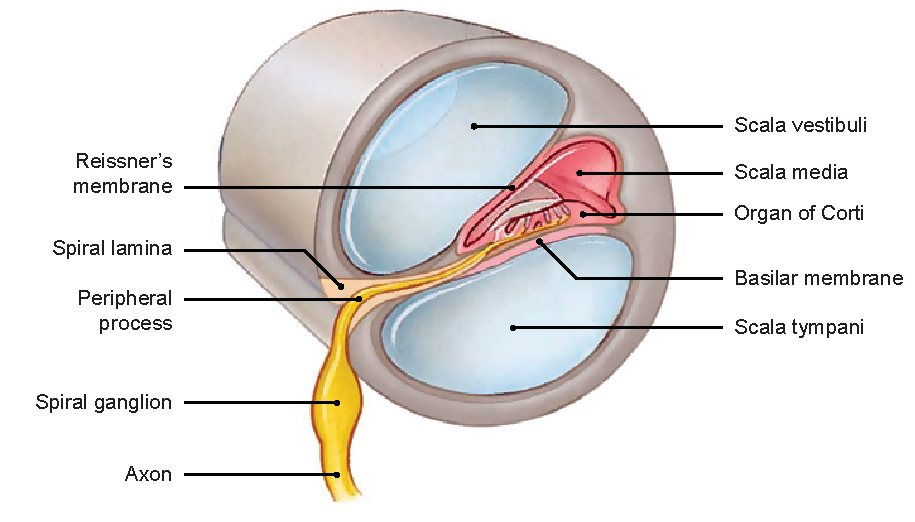
\includegraphics[width=14.6cm]{Background/cochlear_turn}
	\caption[Sectional view through one turn of the cochlea]{Sectional view
	through one turn of the cochlea. (Image adapted from
	Tate~\cite{tate2012}. Copyright \textcopyright{} 2012, McGraw Hill.)}
	\label{fig:cochlea}
\end{figure}

The upper and lower boundaries of the scala media are formed by two thin
membranes---\emph{Reissner's membrane} and the \emph{basilar membrane}---which
separate it from the scala vestibuli and the scala tympani, respectively. Its
lateral border is the \emph{spiral ligament}, which is attached to the bone of
the lateral wall (Figure~\ref{fig:corti}). A capillary bed known as the
\emph{stria vascularis} forms on the upper portion of the spiral ligament at its
junction with the scala media. Along with the spiral ligament and the epithelial
supporting cells, the stria vascularis plays an important role in maintaining
the ionic composition of the endolymphatic space~\cite{flint2010}.

\begin{figure}[p]
	\centering
	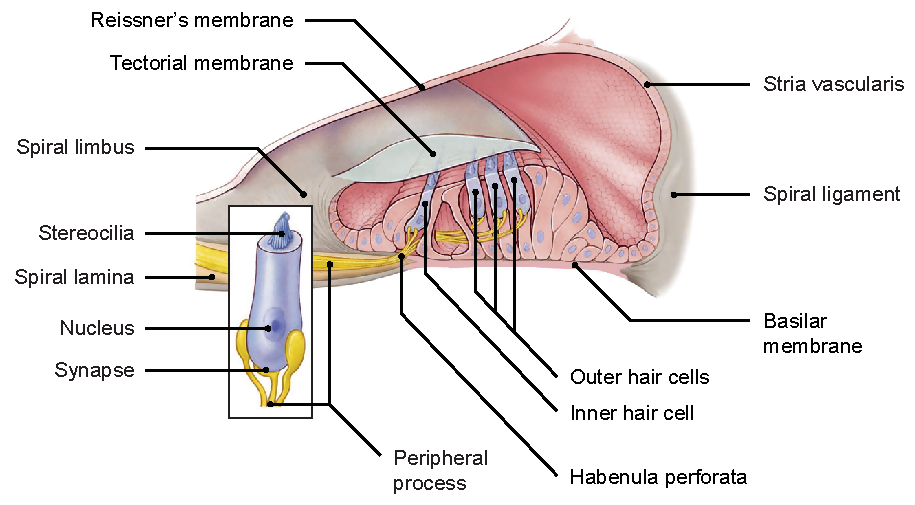
\includegraphics[width=15cm]{Background/corti_hair_cell}
	\caption[The organ of Corti]{The organ of Corti within the scala media.
	Inset shows the basic structure of an isolated hair cell. (Image adapted from
	Tate~\cite{tate2012}. Copyright \textcopyright{} 2012, McGraw Hill.)}
	\label{fig:corti}
\end{figure}

The scala media only spans part of the radial distance from the lateral wall to
the bony core of the cochlea, known as the \emph{modiolus}. The remaining
distance is occupied by the \emph{spiral lamina}, a double-layer bony plate that
extends outwards from the modiolus to meet the basilar membrane. The space
between the plates is occupied by the auditory neurons as they pass through to
the modiolus, as detailed in the next section.

All of these structures together wrap around the modiolus along the helical path
of the scalae. Starting from the round window, the first four quadrants comprise
the basal turn, the next four the middle turn, and the remainder the apical
turn. Erixon \etal~\cite{erixon2009} studied 73 corrosion casts of adult human
inner ears and found that an average human cochlea has 2.6 turns. The
observed range of 2.2--2.9 turns indicates considerable variation between
individuals. The study also revealed variations in other key dimensions; these
measurements are summarised in Table~\ref{table:cochlea_dimensions}.

\begin{table}
	\centering
	\sffamily
	\small
	
	\caption[Key dimensions of the adult human cochlea]{Key dimensions of the adult
	human cochlea. (Data from Erixon~\etal~\cite{erixon2009}.)}
	\label{table:cochlea_dimensions}
	
	\begin{subtable}[t]{0.47\textwidth}
        \caption{Outer wall length.}
        \label{table:dimensions_outer_wall}

        \begin{tabularx}{\textwidth}{X c c}
			\toprule
			\textbf{Location} 	& \textbf{~~Mean $ \boldsymbol\pm $ SD~~}	& \textbf{~~~Range~~~~}\\
								& \textbf{(mm)}								& \textbf{(mm)} \\
			\midrule
			
			First turn		& 22.6 $ \pm $ 0.83 		& 20.3--24.3\\
			Second turn		& 12.4 $ \pm $ 0.63 		& 10.7--13.3\\
			Third turn		& 6.1 $ \pm $ 1.40			& 1.5--8.2\\[1.5mm]
			\emph{Total}	& 42.0 $ \pm $ 1.96			& 38.6--45.6\\
			
			\bottomrule
		\end{tabularx}
		
    \end{subtable}
    
    \vspace{1em}
	\begin{subtable}[t]{0.47\textwidth}
        \caption{Height.}
        \label{table:dimensions_height}

        \begin{tabularx}{\textwidth}{X c c}
			\toprule
			\textbf{Location} 	& \textbf{~~Mean $ \boldsymbol\pm $ SD~~}	& \textbf{~~~Range~~~~}\\
								& \textbf{(mm)}								& \textbf{(mm)} \\
			\midrule
			
			First turn		& 2.1 $ \pm $ 0.20			& 1.6--2.6\\
			Second turn		& 1.2 $ \pm $ 0.17 			& 0.8--1.6\\
			Third turn		& 0.6 $ \pm $ 0.18 			& 0.3--1.1\\[1.5mm]
			\emph{Total}	& 3.9 $ \pm $ 0.37 			& 3.3--4.8\\
			
			\bottomrule
		\end{tabularx}
		
    \end{subtable}
    
    \vspace{1em}
	\begin{subtable}[t]{0.47\textwidth}
        \caption{Width.}
        \label{table:dimensions_width}

        \begin{tabularx}{\textwidth}{X c c}
			\toprule
			\textbf{Location} 	& \textbf{~~Mean $ \boldsymbol\pm $ SD~~}	& \textbf{~~~Range~~~~}\\
								& \textbf{(mm)}								& \textbf{(mm)} \\
			\midrule
			
			First turn		& 6.8 $ \pm $ 0.46			& 5.6--8.2\\
			Second turn		& 3.8 $ \pm $ 0.25			& 3.3--4.3\\
			Third turn		& 2.1 $ \pm $ 0.52			& 0.6--3.6\\
			\bottomrule
		\end{tabularx}
		
    \end{subtable}
    
\end{table}

\subsubsection{Neural Structures}

The cornerstone of the hearing mechanism is the hair cell (see inset,
Figure~\ref{fig:corti}) in that these cells are responsible for the actual
transduction of physical vibrations that make up sound waves to neural impulses.
They are housed within the \emph{organ of Corti}, which is named after its
discoverer, Alfonso Corti~\cite{jahn2001}. Figure~\ref{fig:corti} depicts the
positions of the hair cells within the organ of Corti. They are embedded in
epithelial supporting cells that lie on the basilar membrane and are organised
into one inner row and three outer rows. \emph{Stereocilia} protruding from the
exposed surface of each hair cell are attached the overlying \emph{tectorial
membrane}, which itself is anchored to the medial wall of the scala media via
the \emph{spiral limbus}.

There are about 15,000 hair cells in the human inner ear, split into 3,000 inner
hair cells and 12,000 outer hair cells~\cite{nadol1993,flint2010}. These are
monitored by the \emph{peripheral processes} of the bipolar auditory neurons.
The processes leave the organ of Corti and enter the space between the double
wall of the spiral lamina via tiny openings called the \emph{habenula
perforata}. From here, they travel centrally to Rosenthal's canal, wherein the
cell bodies of the neurons lie and together form the spiral ganglion. Their
myelinated axons then run towards the base of the cochlea, combining to form the
cochlear branch of N VIII. Most of the auditory neurons are afferent, but there
are also some efferent fibres that lead back towards the hair cells to form a
feedback loop.

\subsubsection{Vascular Structures}
\label{sect:cochlear_vessels}

Traditional descriptions of the cochlea have generally excluded its vasculature.
The most comprehensive investigation of the cochlear vessels is a survey by
Axelsson~\cite{axelsson1968}, which encompassed work by pioneers such as
Ibsen~\cite{ibsen1881} and Schwalbe~\cite{schwalbe1887} in the 19th century on
animal specimens, as well as later studies of the human system by
Eichler~\cite{eichler1892}, Siebenmann~\cite{siebenmann1894},
Nabeya~\cite{nabeya1923}, and Scuderi and Del Bo~\cite{scuderi1952}. The
information provided by these authors was at times incomplete and
conflicting~\cite{axelsson1968}, which is not unexpected given the limitations
in existing imaging technology and the complexity of the cochlear vasculature
(cf. Siebenmann's illustration in Figure~\ref{fig:siebenmann}). Axelsson went on
to unify the previous work, so the information in the remainder of this section
is drawn predominantly from his account.

\begin{figure}
	\centering
	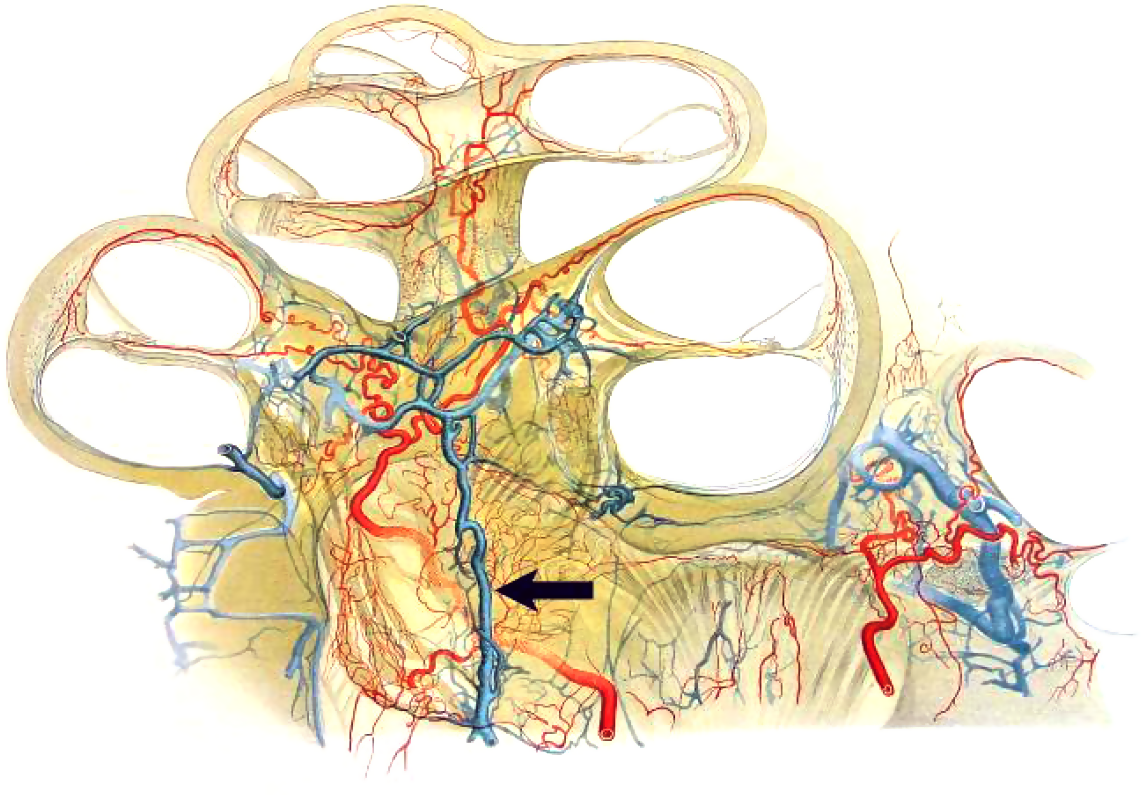
\includegraphics[height=7.5cm]{Background/siebenmann}
	\caption[Sketch of the cochlear vasculature]{Sketch of the cochlear vasculature
	by Siebenmann, demonstrating the intricate structure of the blood vessel
	network. The black arrow indicates the ``central auditory vein'', which likely
	refers to what is now termed the ``common modiolar vein'' (cf.
	Figure~\ref{fig:venous_drainage}). (Source: Siebenmann~\cite{siebenmann1894}.)}
	\label{fig:siebenmann}
\end{figure}

The origin of the cochlear blood supply can be traced back to the
\emph{brachiocephalic trunk}. From here, the arterial path typically follows the
vertebral, basilar, anterior inferior cerebellar, and labyrinthine arteries in
order as shown in Figure~\ref{fig:arterial_supply}, though slight variations may
exist amongst individuals. In either case, the \emph{labyrinthine artery} is
usually the sole supplier of blood to the cochlea. It follows N VIII through the
\emph{internal acoustic meatus}, and branches to form the \emph{anterior
vestibular artery} (AVA) and the \emph{common cochlear artery}. The latter then
divides into the \emph{vestibulo-cochlear artery} (VCA) and the \emph{spiral
modiolar artery} (SMA).

\begin{figure}
	\centering
	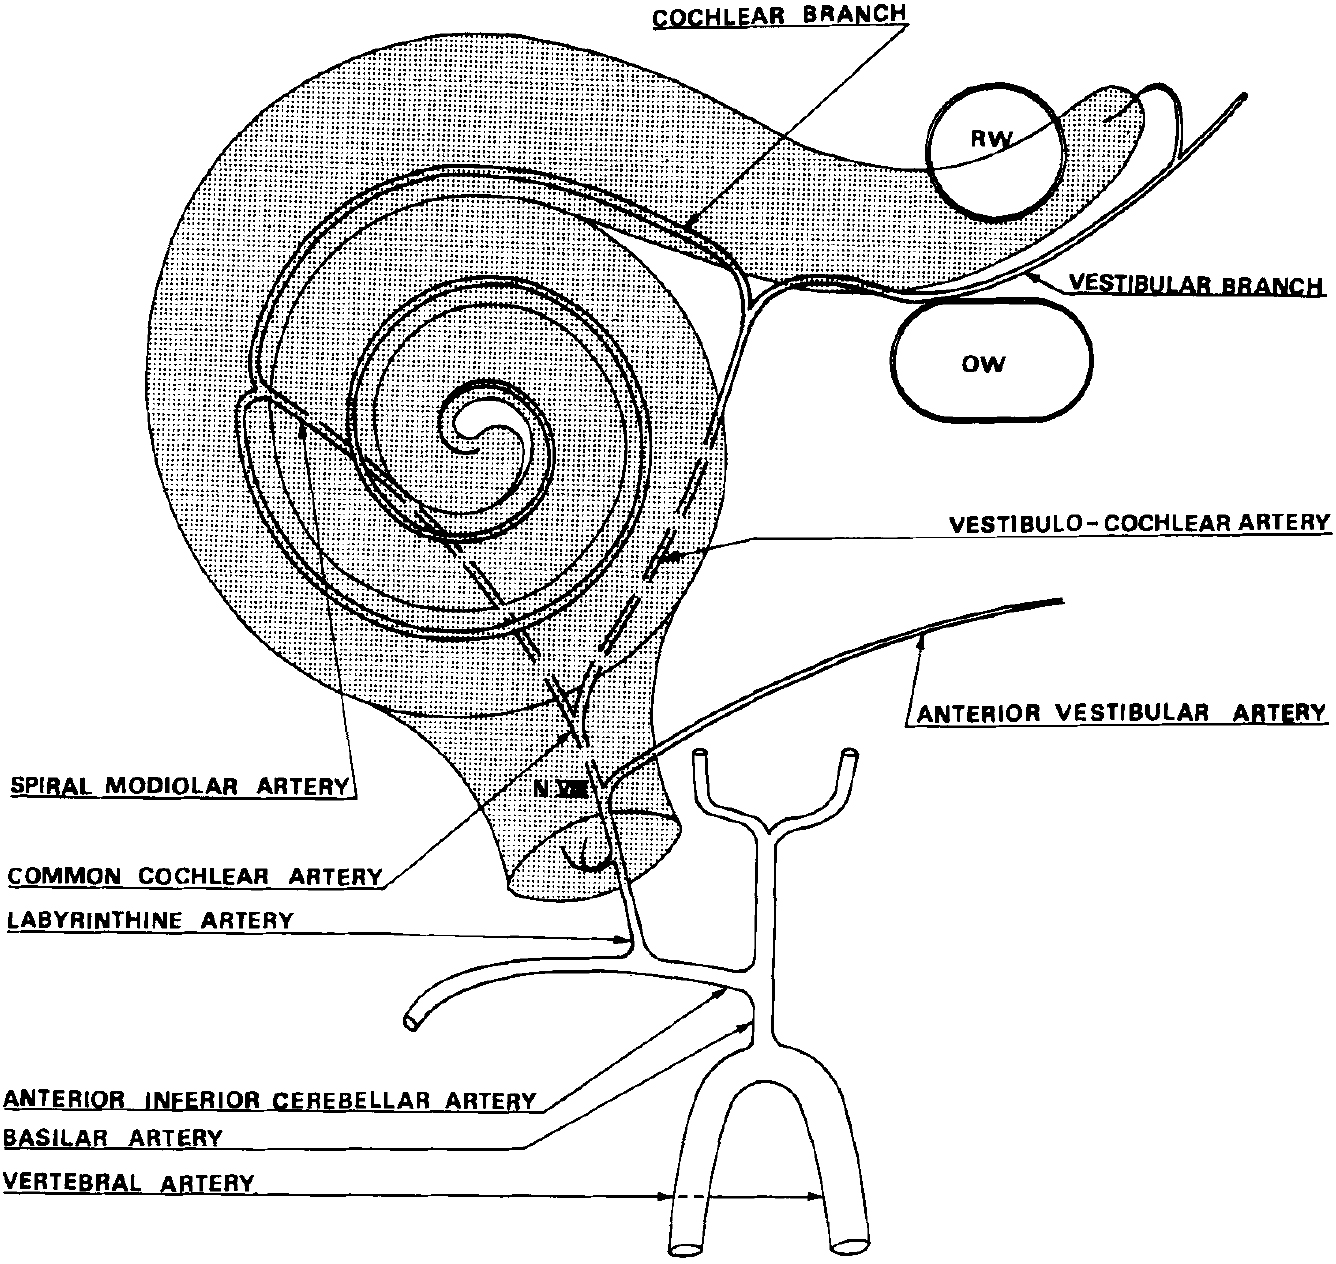
\includegraphics[height=11.5cm]{Background/arterial_supply}
	\caption[Schematic of the cochlear arterial supply in man]{Schematic of the
	cochlear arterial supply in man. OW=oval window; RW=round window; N
	VIII=vestibulocochlear nerve. (Source: Axelsson~\cite{axelsson1968}. Copyright
	\textcopyright{} 1968, Taylor \& Francis.)}
	\label{fig:arterial_supply}
\end{figure}

Each of these three terminal branches leads to a different region of the inner
ear. The AVA supplies the posterior vestibule and the lateral and anterior
semicircular canals~\cite{leblanc1999}. The VCA enters the modiolus near the
bottom of the basal turn and splits into the \emph{vestibular branch} and the
\emph{cochlear branch}, which run basally and apically along the spiral
respectively. The former supplies the basal-most end of the cochlea, the
posterior semicircular canal and the vestibule, while the latter supplies about
a third of the basal turn before anastomosing with the SMA. This third terminal
branch supplies the remaining majority of the cochlea and is therefore the most
important.

Upon entering the second quadrant of the basal turn, the SMA runs apically,
spiralling around the nerve trunk until it reaches the helicotrema (see
Figure~\ref{fig:modiolar_vessels}). Internal and external \emph{radiating
arterioles} regularly branch off normal to the helical path, feeding capillary
beds in the modiolus, the spiral lamina and the external wall. The capillaries
rejoin, forming \emph{collecting venules} that drain into the cochlear veins.
These radial vessels are shown in Figure~\ref{fig:rad_vessels}.

\begin{figure}
	\centering
	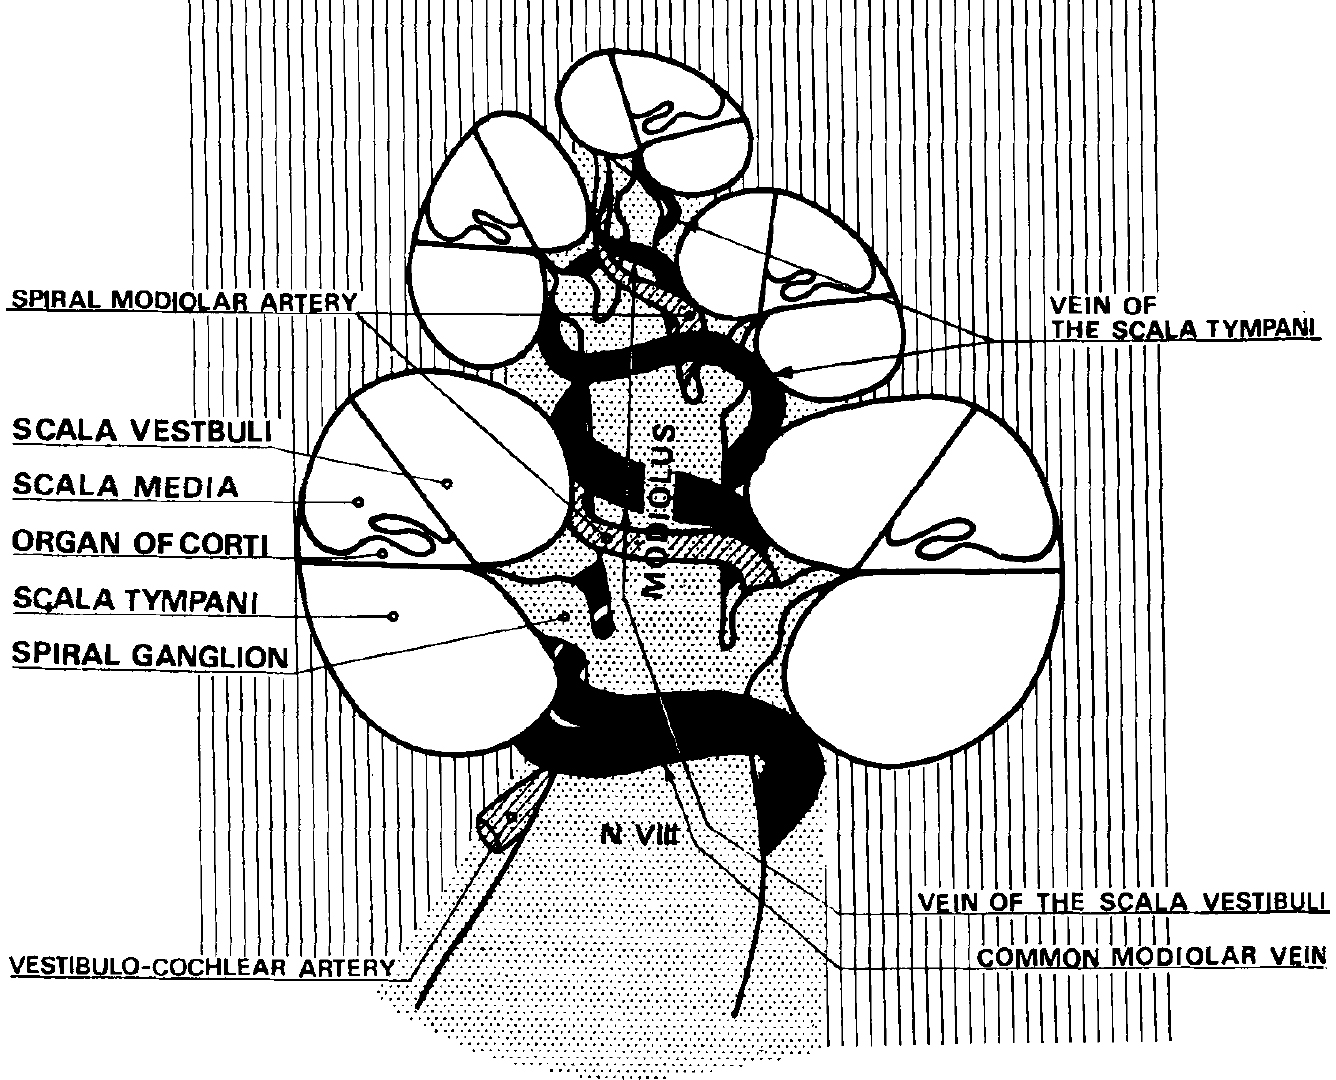
\includegraphics[height=9.2cm]{Background/modiolar_vessels}
	\caption[Cross-sectional schematic of the modiolar vessels in
	man]{Cross-sectional schematic of the modiolar vessels in man. (Source:
	Axelsson~\cite{axelsson1968}. Copyright \textcopyright{} 1968, Taylor \&
	Francis.)}
	\label{fig:modiolar_vessels}
\end{figure}

\begin{figure}
	\centering
	
    \begin{subfigure}[t]{0.53\textwidth}
        \centering
        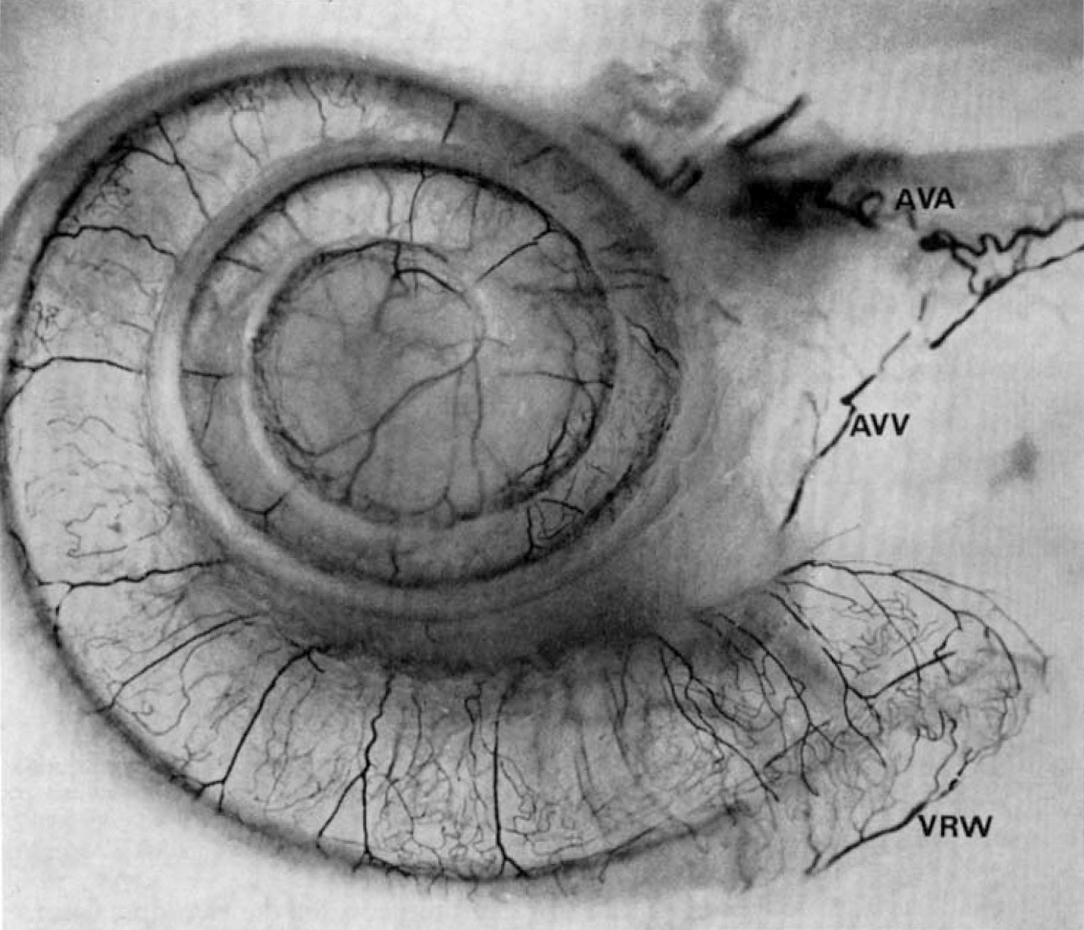
\includegraphics[height=6.5cm]{Background/radart}
        \caption{ }
        \label{fig:rad_art_top}
    \end{subfigure}
	~
	\begin{subfigure}[t]{0.45\textwidth}
        \centering
        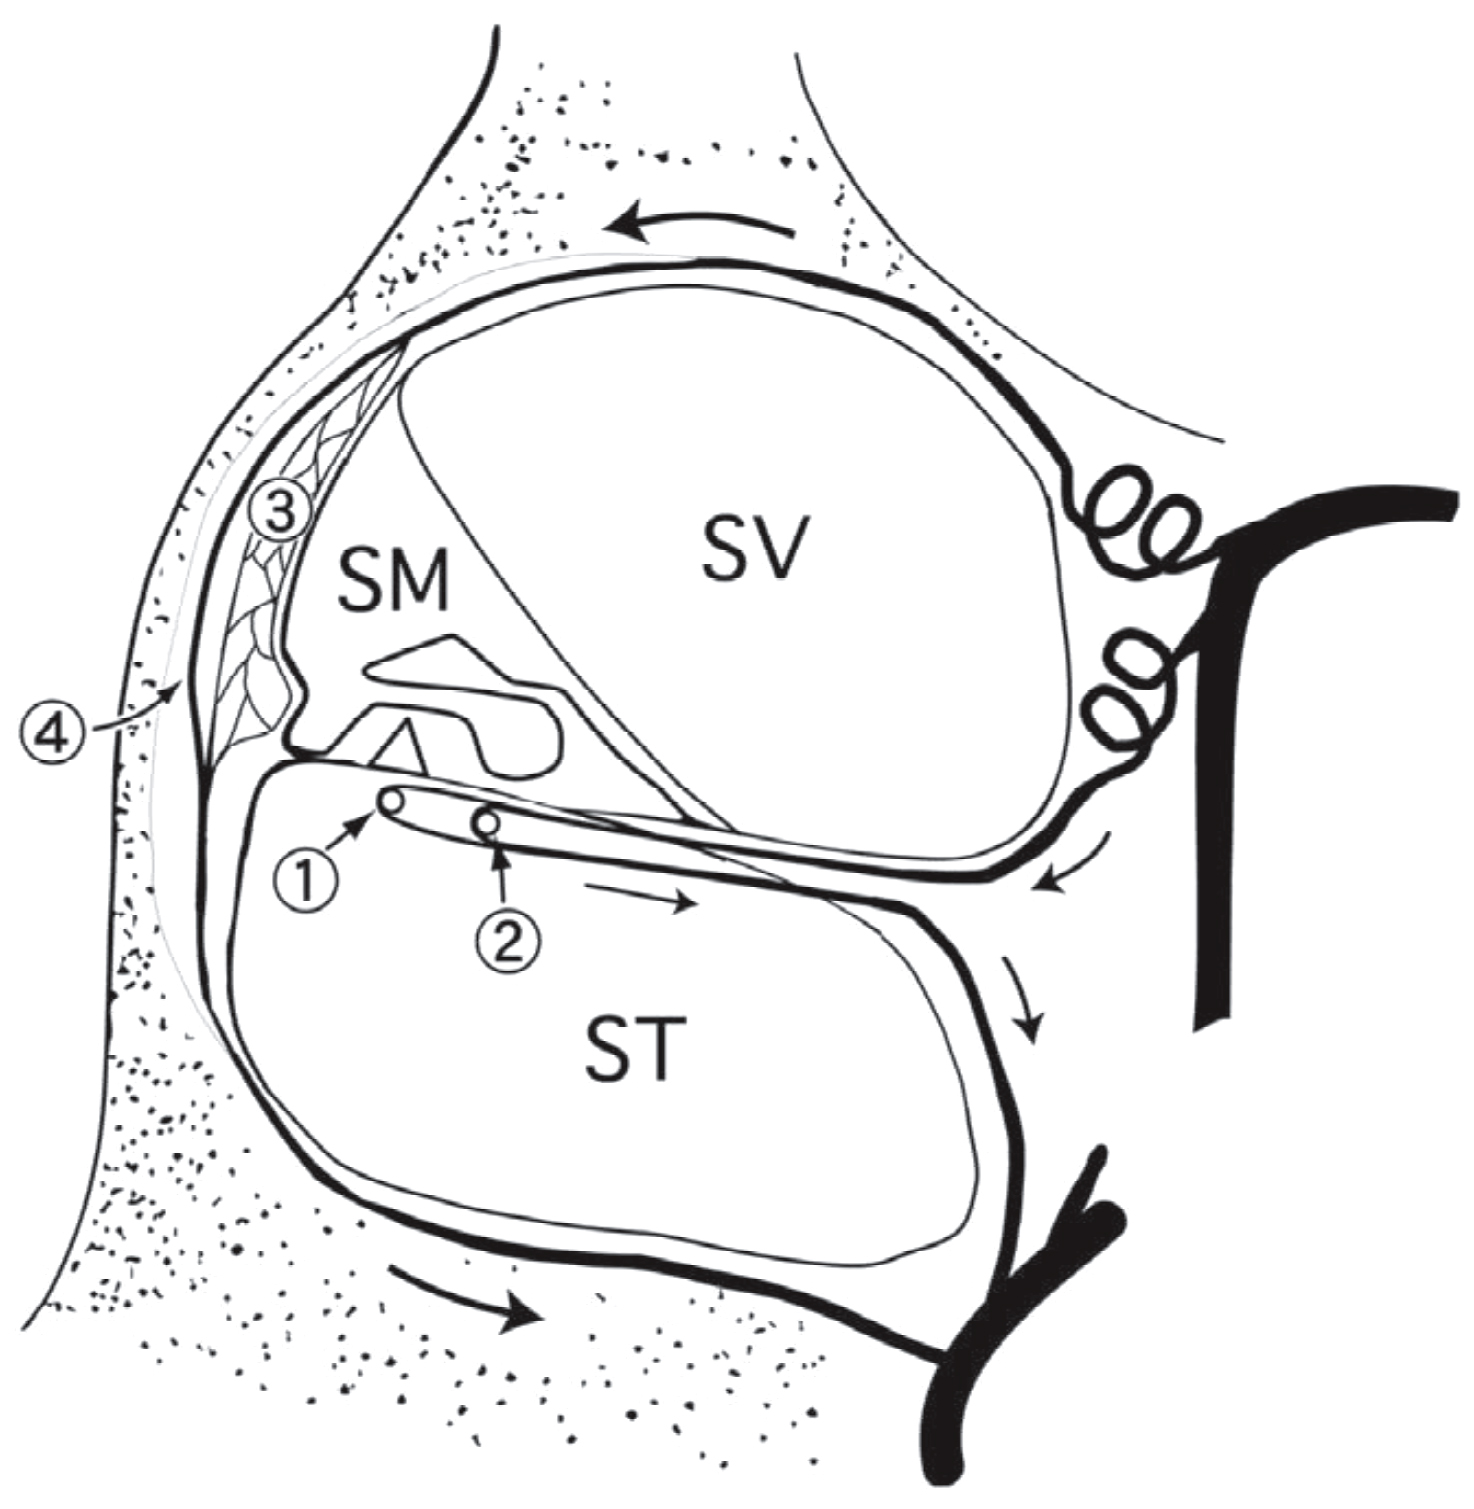
\includegraphics[height=6.5cm]{Methodology/vesselsinturn}
        \caption{ }
        \label{fig:rad_art_section}
    \end{subfigure}
    
	\caption[Radiating arterioles and collecting venules]{(a) Radiating arterioles
	(darker) and collecting venules (lighter) in the human cochlea. AVA=anterior
	vestibular artery; AVV=anterior vestibular vein; VRW=vein of the round window.
	(Source: Axelsson~\cite{axelsson1968}. Copyright \textcopyright{} 1968, Taylor
	\& Francis.) (b) Schematic view through one turn of the cochlea. (Source:
	Nakashima~\etal~\cite{nakashima2003}. Copyright \textcopyright{} 2003, Elsevier
	B.V.)}
	\label{fig:rad_vessels}
\end{figure}

Human cochleae exhibit a double venous system, one for the scala vestibuli and
one for the scala tympani. The former is drained along with the spiral lamina by
a discontinuous series of venous segments together known as the \emph{vein of
the scala vestibuli} (VSV), which is located centrally in the modiolar wall (see
Figures~\ref{fig:modiolar_vessels} and \ref{fig:venous_drainage}). Likewise, the
latter is drained with the spiral ganglion and the external wall of the scala
media by the similarly-structured \emph{vein of the scala tympani} (VST). The
VSV and VST merge near the first quadrant of the basal turn to form the common
modiolar vein (CMV). More basally, the \emph{vein of the round window} (VRW)
drains the associated collecting venules. Both the VRW and the CMV join with the
vestibulo-cochlear vein (VCV) to become the vein of the cochlear aqueduct
(VCAQ), which leaves the cochlear region.

\begin{figure}
	\centering
	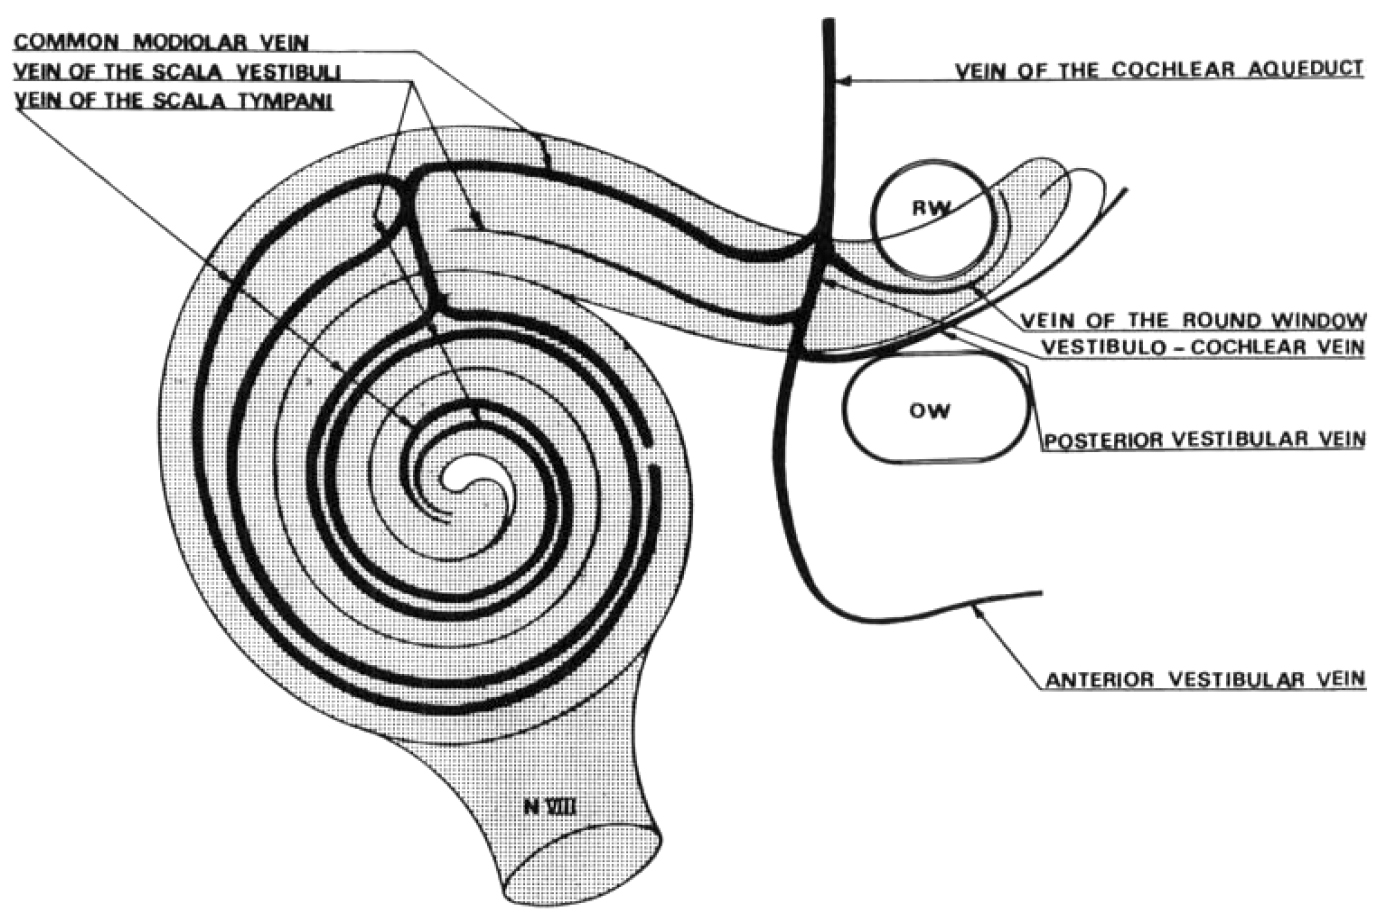
\includegraphics[height=9.2cm]{Background/modiovein}
	\caption[Schematic of the cochlear venous drainage in man]{Schematic of the
	cochlear venous drainage in man. OW=oval window; RW=round window; N
	VIII=vestibulocochlear nerve. (Source: Axelsson~\cite{axelsson1968}. Copyright
	\textcopyright{} 1968, Taylor \& Francis.)}
	\label{fig:venous_drainage}
\end{figure}

Reissner's membrane and some parts of the organ of Corti are avascular.

\subsection{Comparison of Human and Guinea Pig Cochleae}
\label{sect:comparison_of_species}

Although the ultimate goal of cochlear implant (CI) research is to restore the
perception of hearing in humans, the anatomical surroundings of the human
cochlea make \invivo{} testing challenging. The otic capsule surrounding the
cochlea is both thick and extremely dense, and its location deep within the
petrous part of the temporal bone impedes surgical access. Experimental
implantation and probing is unwarranted given the high ratio of risk to benefit.
Cadaveric studies are one alternative, but changes in both the shape and
properties of the tissues post-mortem impede the extrapolation of insights to
living subjects~\cite{ifukube1987,kral1998}.

% The taking of measurements requires probes to be placed within the region of
% interest, but the temporal bone and otic capsule surrounding the cochlea impede
% surgical access. It is possible to penetrate these bones with the correct
% surgical tools, but even then, the phyical invasion of the probes into the
% tissue space would compromise the integrity of the cochlear structures and
% change the measured potentials relative to a true \invivo{} implant. There would
% also be challenges in controlling the positioning of the probe to accurately
% obtain the large number of sample points required to build a detailed
% electro-anatomical map. Furthermore, there are the ethical concerns of such
% experiments on the health and wellbeing of the subjects, whether human or some
% other animal species. Measurements in cadavers may alleviate some of these
% concerns, but physiological changes post-mortem introduce a host of other
% inaccuracies.

Since the mammalian cochlea is similar in both structure and function across
species, many CI studies have been performed on animals---typically cats and
guinea pigs, but also mice, gerbils, rats, chinchillas, and
monkeys~\cite{axelsson1968,greenwood1990,kral1998,zeng2004}. The cochlea of the
guinea pig is commonly used because it is relatively large~\cite{zeng2004} and,
unlike the human cochlea, it is easily exposed in the tympanic
bulla~\cite{cooper1975} (see Figure~\ref{fig:guinea_pig_bulla}), allowing
experimental measurements to be taken relatively easily.
Miyamoto~\cite{miyamoto1986} noted that guinea pig cochleae serve as ``an
appropriate experimental animal model for\ldots[electrophysiological studies] of
cochlear function''.

\begin{figure}[p]
	\centering
	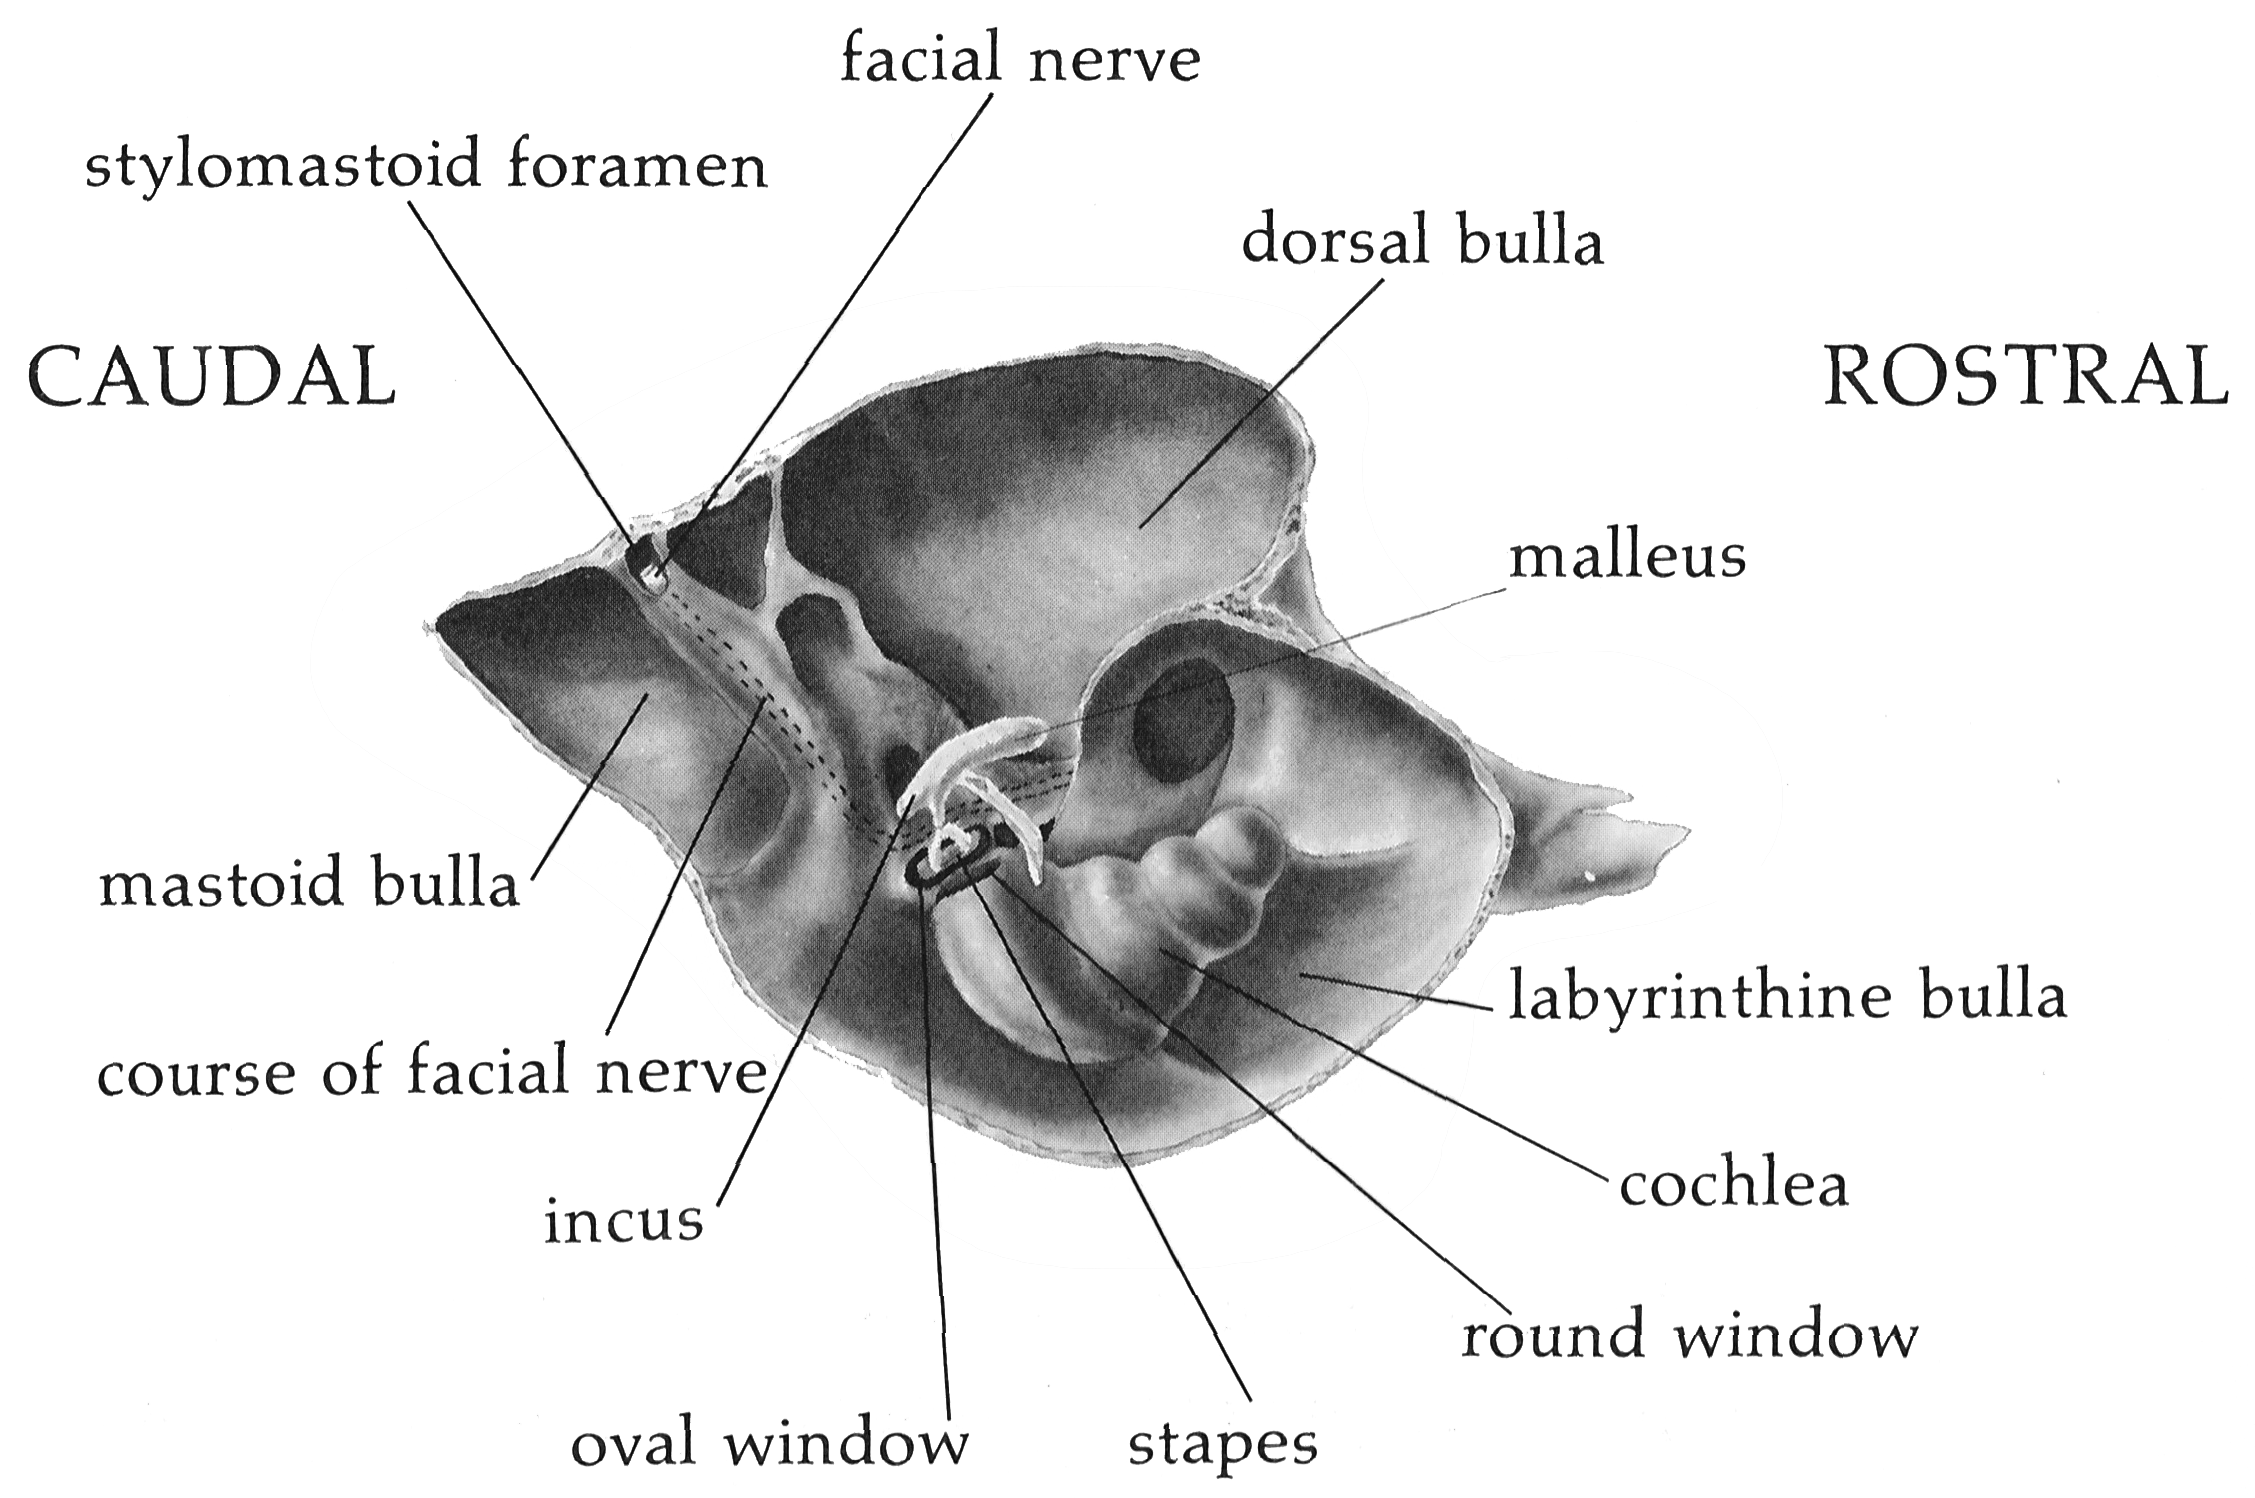
\includegraphics[height=7cm]{Validation/tympanic_bulla}
	\caption[Internal aspect of the tympanic bulla]{Internal aspect of the
	tympanic bulla in the guinea pig. Note how the lateroapical portion of the
	cochlea protrudes into the air space of the tympanic bulla. (Source: Cooper and
	Schiller~\cite{cooper1975}. Copyright \textcopyright{} 1975, Harvard
	University Press.)}
	\label{fig:guinea_pig_bulla}
\end{figure}

Like other mammals, the cochleae of both humans and guinea pigs are comprised
of the cross-sectional structures shown in Figures~\ref{fig:cochlea} and
\ref{fig:corti} spiralling around a nerve-filled modiolus. There are several
notable differences relative to the human cochlea; the main ones are listed in
Table~\ref{table:cochleae_comparison}.

% \item has a relatively large endolymphatic space (by percentage volume) in both
% the cochlea proper and the semicircular canals~\cite{thorne1999};

\begin{table}[p]
	\centering
	\sffamily
	\small
	
	\caption[Comparison of human and guinea pig cochleae]{Comparison of human and
	guinea pig cochleae. Data compiled from various
	sources~\cite{black1980,ota1980,nadol1988comparative,thorne1999,frijns2001,erixon2009}.}
	\label{table:cochleae_comparison}
	
    \begin{tabular}{p{4.5cm} p{4.0cm} p{5.2cm}}
		\toprule
		\textbf{Attribute}	& \textbf{Human}	& \textbf{Guinea pig} \\
		\midrule
		
		Number of turns				& 2.2--2.9				& 3.5--4 \\
		Scalae length				& 26--28~mm				& $ \approx $16~mm \\
		Volume of scala tympani		& 29~$ \upmu $L			& 4.8~$ \upmu $L \\
		Myelination	of spiral ganglion cell bodies		& Rare ($<$5\%) &	Mostly
			myelinated \\
		Geometry of basal end		& Follows spiral trajectory
									& Hooked (turns more parallel with cochlear axis) \\ 
		Location within bone		& Embedded except for the round and oval windows
									& Apex protrudes into tympanic bulla \\
		\bottomrule
	\end{tabular}
		
\end{table}

Since the guinea pig cochlea is not embedded within the petrous part of the
temporal bone, different current pathways are expected~\cite{kral1998}.
These differences mean that although the modelling results may be indicative,
care must be taken when extrapolating results from one species to
another~\cite{frijns2001}.

% ==============================================================================

\section{Hearing Physiology}

\subsection{Normal Hearing}
\label{sect:normal_hearing}

Normal hearing is comprised of two distinct stages: the first (sensation) occurs
when a sound stimulus is detected at the biological receptor; the second
(perception) occurs when a conscious awareness of the sensation is
obtained~\cite{martini2006}. Sensation is therefore clearly a prerequisite for
perception, and any complications in sensing a sound stimulus flow on to impair
the perception of that sound.

The propagation of sound waves through the cochlea is illustrated in
Figure~\ref{fig:travelling_wave}. Sound stimuli consist of pressure waves moving
through a medium, typically air or water. They are funnelled into the external
acoustic meatus by the auricle and detected by the tympanic membrane, which
vibrates in response. These vibrations are mechanically coupled by the auditory
ossicles to the oval window, where the action of the stapes footplate induces
compressional waves in the perilymph. The 20:1 area ratio between the tympanic
membrane and the stapes footplate and the 1.31:1 lever ratio between the moment
arms of the malleus and the incus help to minimise the loss of energy that would
otherwise occur due to the large difference in acoustic impedances between air
and perilymph~\cite{flint2010}.

\begin{figure}
	\centering
	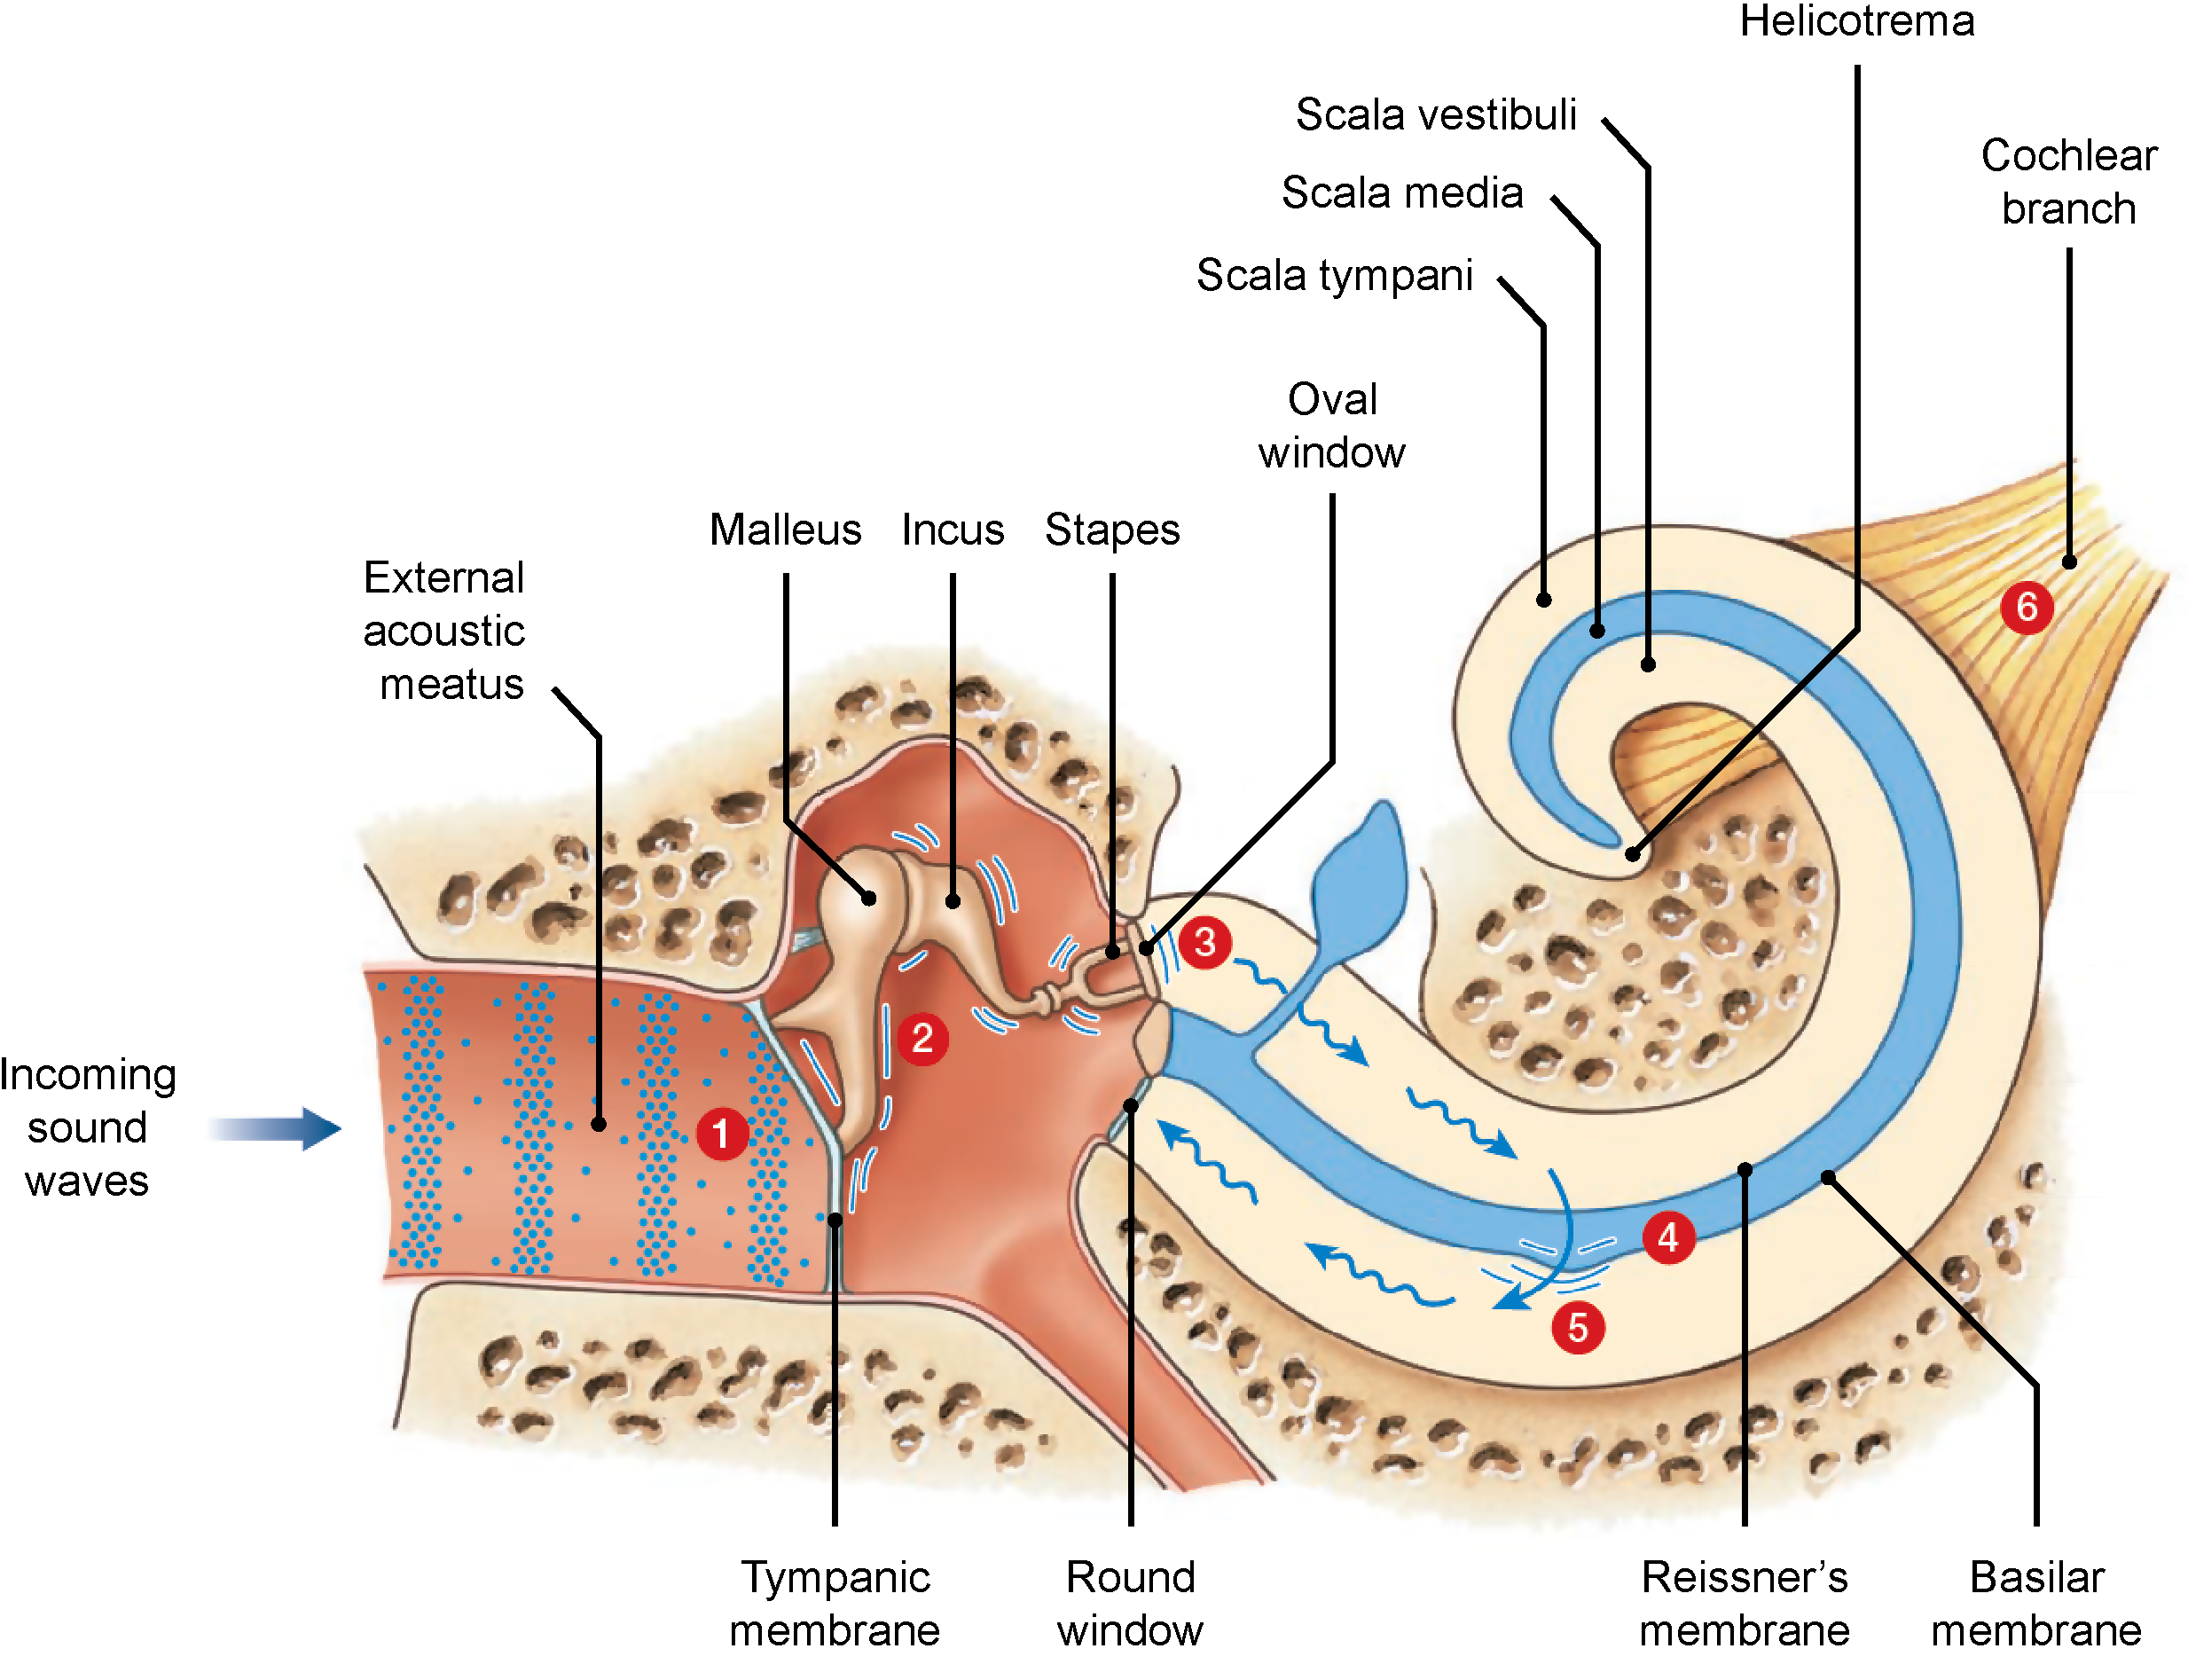
\includegraphics[width=\textwidth]{Background/normal_hearing.pdf}
	\caption[Sound wave propagation in the cochlea]{Sound wave propagation in the
	cochlea. Vibrations in the air are (1) received by the tympanic membrane, (2)
	transmitted via the ossicles to the oval window, and (3) travel up the scala
	vestibuli towards the helicotrema. For each frequency component, the
	travelling wave (4) peaks at a characteristic location along the cochlear
	partition and stimulates the corresponding hair cells, before (5) continuing
	via the scala tympani towards the round window, where the displacement is
	dissipated. Action potentials triggered by hair cell stimulation are (6) sent
	via the cochlear nerve to the auditory cortex for processing. (Image adapted
	from Martini~\etal\cite{martini2006}. Copyright \textcopyright{} 2006,
	Daryl Fox.)}
	\label{fig:travelling_wave}
\end{figure}

Sound waves travel up through the scala vestibuli to the helicotrema and return
via the scala tympani, generating a pressure gradient that distorts the organ of
Corti and the basilar membrane (together called the \emph{cochlear partition}).
Von B{\'e}k{\'e}sy~\cite{vonbekesy1960} showed that this \emph{travelling wave}
peaks at different locations along the basilar membrane due to its varying
stiffness, with higher frequencies peaking at the base and progressively lower
frequencies toward the apex as per Figure~\ref{fig:tonotopy}. As the cochlear
partition is deflected by the travelling wave, relative movement between the
tectorial membrane and the hair cells of the organ of Corti causes displacement
of the stereocilia. Displacement toward the tallest row opens ion channels in
the stereocilia, and the subsequent influx of cations depolarises the hair cell
(Figure~\ref{fig:stereocilia}). This in turn opens the calcium channels at the
base of the hair cell near the afferent nerve fibres, triggering the release of
neurotransmitters across the synapse and inducing action potentials in the
peripheral process of the auditory nerves. Displacement in the opposite
direction leads to hyperpolarisation. Neural excitation is discussed is more
detail in \S\ref{sect:neural_excitation}.

\begin{figure}
	\centering
	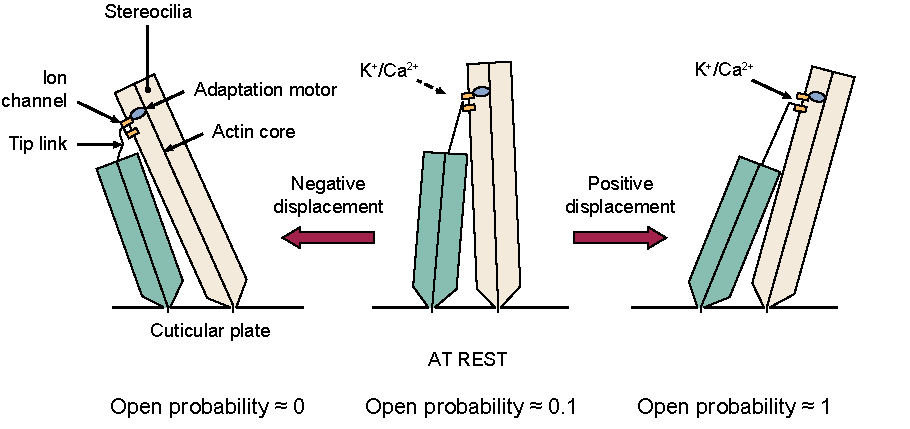
\includegraphics[width=15cm]{Background/stereocilia}
	\caption[Effect of stereocilia movement on ion channels]{Effect of stereocilia
	movement on ion channels. Displacement toward the tallest row stretches
	the spring-link tip links, opening the cation channels and leading to
	depolarisation of the hair cell. (Image adapted from
	Flint~\etal\cite{flint2010}. Copyright \textcopyright{} 2010, Mosby.)}
	\label{fig:stereocilia}
\end{figure}

According to the commonly accepted \emph{place theory} of pitch perception, hair
cells only respond to the frequency component which peaks at their particular
location along the basilar membrane. In this way, the cochlea can be thought of
as a mechanical Fourier transformer that directly extracts a spectral
representation from the sound stimulus~\cite{vonbekesy1960}. The correlation
between characteristic frequency and location (both along the cochlear partition
and in the auditory cortex) is termed the \emph{tonotopic organisation} of the
cochlea, and has been documented for several mammalian species by
Greenwood~\cite{greenwood1990}.

In the final stage, action potentials are relayed via N VIII to the auditory
cortex of the brain. It is there that the signals are decoded and interpreted,
giving rise to a conscious awareness of the original stimulus (i.e. sound
perception).

% ==============================================================================

\subsection{Hearing Loss}
\label{sect:hearing_loss}

Any reduction in the ability of an individual to perceive sound naturally is
known as hearing loss. There are two main categories: \emph{conductive hearing
loss} and \emph{sensorineural hearing loss}. A small proportion of affected
individuals suffer from \emph{mixed hearing loss}, where both of these cases are
exhibited.

Conductive hearing loss (CHL) occurs when there is a problem in the outer or
middle ear. Such conditions prevent vibrations in the air from being
mechanically transmitted through to the inner ear. Common causes of CHL include
obstruction of the external auditory meatus or of the auditory tube, thickening
or perforation of the tympanic membrane, bacterial or viral infections of the
middle ear, and fixation or decoupling of the auditory
ossicles~\cite{nadol1993,economics2006,flint2010}.

Sensorineural hearing loss (SHL) occurs when there is a problem with the
cochlea, the auditory nerve, or the auditory cortex. These locations are
downstream in the hearing chain, so SHL can manifest in individuals with a
normal outer and middle ear. The former is the most common and generally results
from damage to or degeneration of the hair cells in the organ of Corti. Common
causes of SHL include congenital malformations, exposure to excessive noise,
hair cell attrition due to aging (known as \emph{presbycusis}), and chemical
damage from smoking or medications~\cite{nadol1993,economics2006}. Disorders of
the inner ear vascular supply can also result in SHL~\cite{nadol1993}.

In either case, the degree of impairment can vary from negligible to complete
deafness. Scales are indicative but arbitrary, and can vary amongst authorities.
The classification system used by the World Health Organisation is shown in
Table~\ref{table:hearing_loss_classification}.

\section{Chapter Summary}

The cochlea is one part of the mammalian auditory pathway. It primarily consists
of three spiralling fluid chambers, known as the scalae vestibuli, media, and
tympani. These three chambers are separated by Reissner's membrane and the
cochlear partition (formed by the organ of Corti and basilar membrane)
respectively, and are bordered along the peripheral side by the spiral ligament
and stria vascularis. At the centre of the spiral path is the bony modiolus. The
cochlear nerve enters through the base of the modiolus and unravels to supply
the hair cells in the organ of Corti in a tonotopic manner. The major arteries
and veins of the cochlea also follow a modiolar path, with smaller radial
branches and capillary beds supplying the structures within. This is all
surrounded by the incredibly dense otic capsule, and is embedded in the petrous
portion of the temporal bone.

The overall structure is similar between humans and guinea pigs, but naturally
there are differences in geometry between species. Nonetheless, processes
leading to sound perception are the same. Sound entering a normal hearing
cochlea is picked up by the hair cells and transduced into a series of action
potentials that are interpreted by the brain. Unfortunately, this ability is
impaired in some individuals. For those with profound SHL due to hair cell
damage, the only successful treatment is a hearing prosthesis known as the
cochlear implant.

\clearpage

% ==============================================================================

% Page style from here up to References
	\pagestyle{fancy}
	\lhead{{\sffamily \MakeUppercase\leftmark}}
	\chead{}
	\rhead{{\sffamily \MakeUppercase\rightmark}}
	\lfoot{}
	\cfoot{{\sffamily \thepage}}
	\rfoot{}

\chapter{Literature Review}

% Textbox
\begin{center}
	\begin{tcolorbox}[title=\boxtitle]
		\begin{itemize}[leftmargin=*,labelindent=2ex,labelsep=1.5ex,itemsep=0pt,parsep=0pt]
		    \item What are cochlear implants?
			\item How does electrical stimulation compare to normal hearing?
			\item What is the state-of-the-art for bioelectric models of the cochlea?
			\item What are the outstanding issues that need to be addressed?
		\end{itemize}
	\end{tcolorbox}
\end{center}

\section{Cochlear Implants}
\label{sect:cochlear_implants}

Cochlear implants (CIs) are hearing prostheses that have been designed and
successfully used to treat severe to profound sensorineural hearing loss (SHL).
Although individuals with defective hair cells are unable to convert sound waves
into the corresponding neural excitation patterns~\cite{clark1996}, their
residual spiral ganglion cells and the corresponding neuronal axons are often
still healthy and functional~\cite{pfingst2011}. These tissues are therefore the
target of hearing restoration efforts. By injecting electric current into the
inner ear, CIs establish an electrochemical gradient in the cochlear tissues
that directly stimulates the afferent auditory nerve
fibres~\cite{nadol1988treatment,brown2001}, bypassing the defective hair cells.
The modular design of the nervous system, along with the plasticity of the brain
itself, enables these artificially induced neuronal impulses to be interpreted
as sound in much the same way as normal hearing~\cite{fallon2008}.

\subsection{Components and Function}

As shown in Figure~\ref{fig:CI_schematic}, most CI systems include both an
external unit (Figure~\ref{fig:nucleus_parts_ext}), which sits on the outside of
the head, and an internal unit (Figure~\ref{fig:nucleus_parts_int}), which is
surgically implanted under the scalp. The implant body is placed into a pocket
that is drilled into the mastoid bone, and the coiled electrode array is
inserted into the scala tympani of the cochlea (Figure~\ref{fig:CI_in_situ}).
The two parts communicate via transcutaneous induction, enabling the battery and
speech processor to be replaced or upgraded without revision surgery.

\begin{figure}[p]
	\centering
	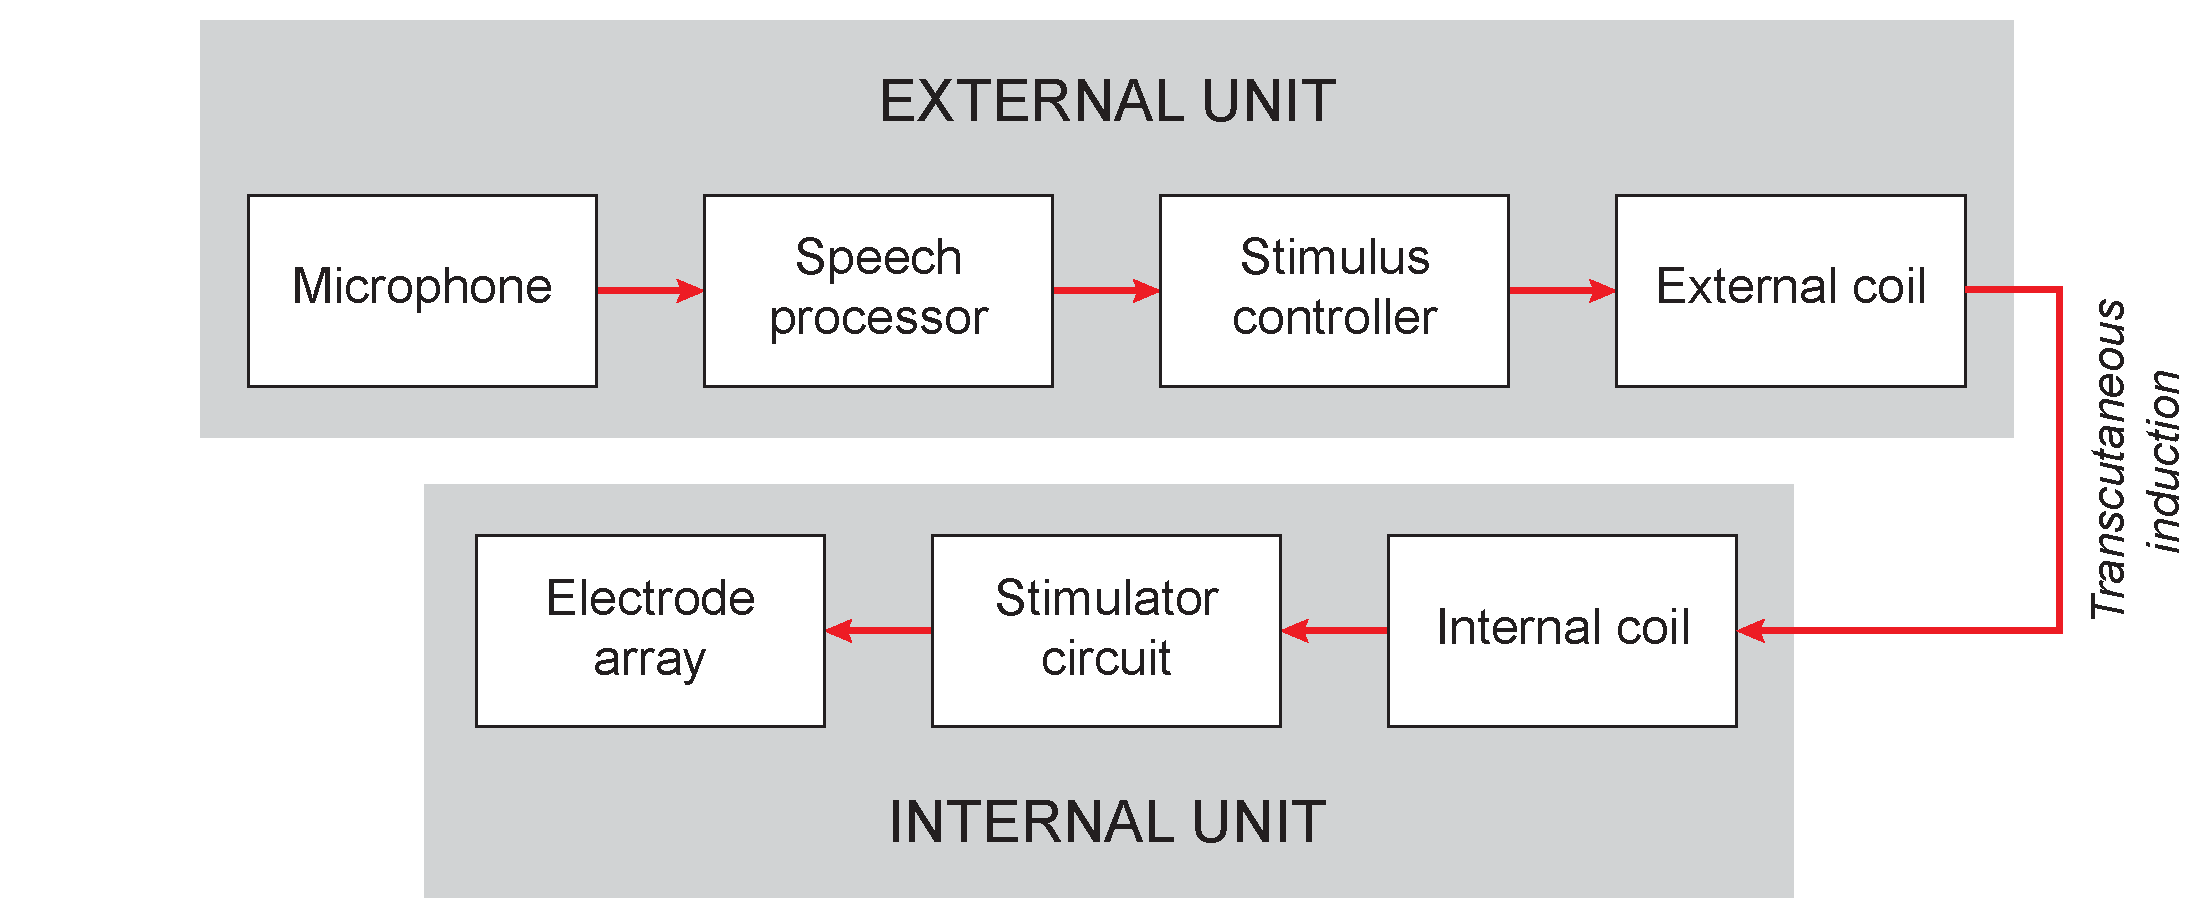
\includegraphics[width=14.5cm]{Background/implant_schematic.pdf}
	\caption[Schematic diagram of a cochlear implant system]{Schematic diagram of a
	cochlear implant system. (Adapted from Webster~\cite{webster1998}.)}
	\label{fig:CI_schematic}
\end{figure}

\begin{figure}[p]
    \centering
    \begin{subfigure}[t]{0.4\textwidth}
        \centering
        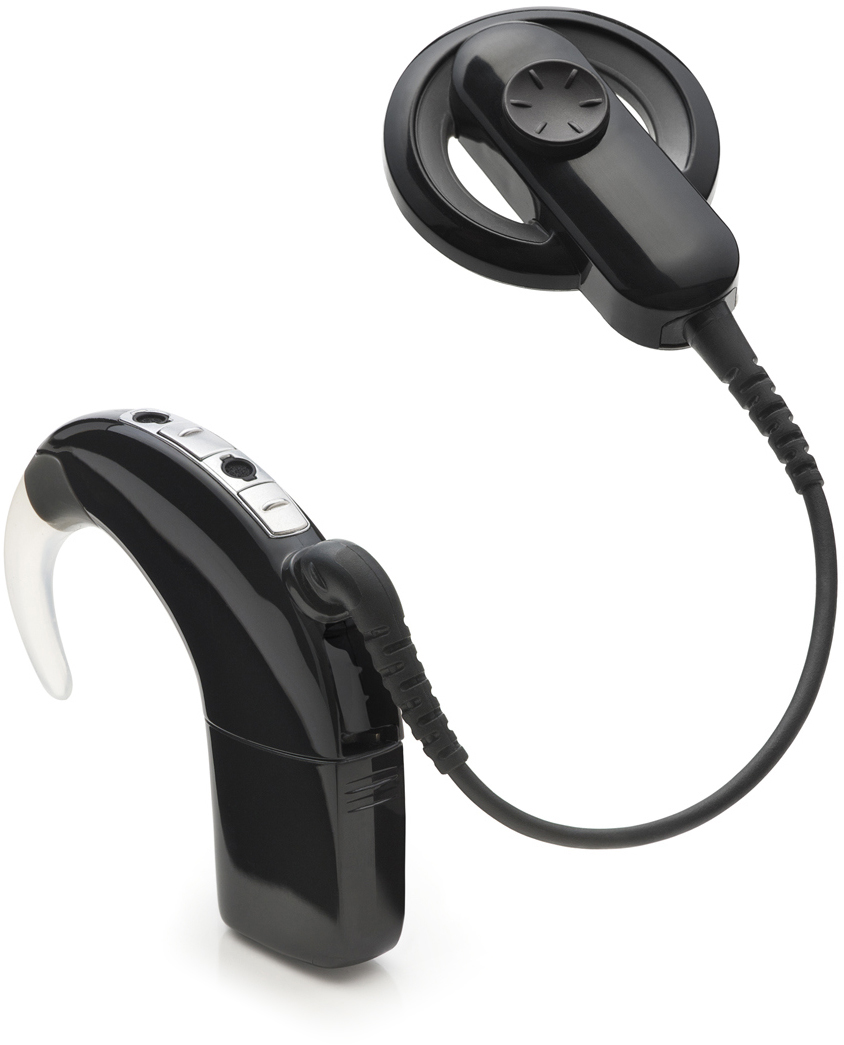
\includegraphics[height=7.5cm]{Background/CI_external_C920}
        \caption{ }
        \label{fig:nucleus_parts_ext}
    \end{subfigure}
    \hspace{1cm}
    \begin{subfigure}[t]{0.4\textwidth}
        \centering
        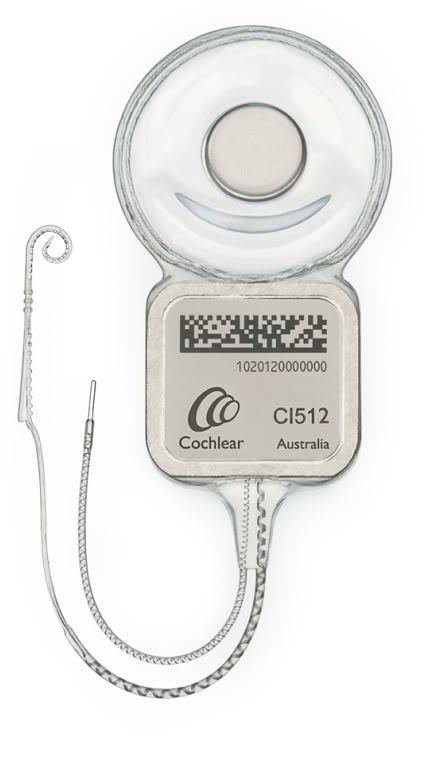
\includegraphics[height=7.5cm]{Background/CI_internal_CI512}
        \caption{ }
        \label{fig:nucleus_parts_int}
    \end{subfigure}
    
	\caption[The Nucleus 6 cochlear implant system by Cochlear Limited]{The Nucleus
	6 cochlear implant system by Cochlear Limited. (a) The external behind-the-ear
	unit, housing the battery, microphone, speech processor, and stimulus
	controller tethered to the external coil. (b) The cochlear implant proper,
	consisting of the internal coil, stimulator circuitry, return electrodes, and
	intracochlear electrode array. The external and internal coils are
	aligned using magnets. (Source:	Cochlear Limited.)}
	\label{fig:nucleus_parts}
\end{figure}

\begin{figure}
	\centering
	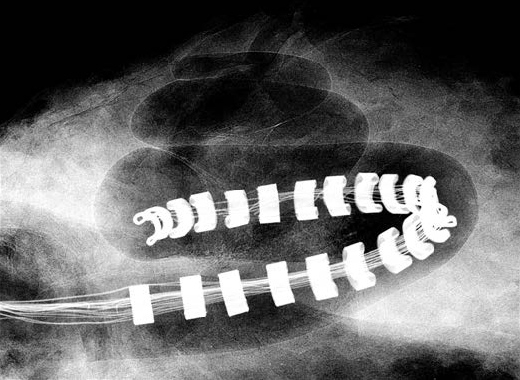
\includegraphics[height=5.8cm]{Background/CI_phase-contrast_x-ray}
	\caption[Phase-contrast x-ray image of an intracochlear electrode array
	\insitu]{Phase-contrast x-ray image of an intracochlear electrode array
	\insitu. Note how the half-banded electrode pads in this design face towards
	the modiolus. (Source: Xu~\cite{xu2001}. Copyright \textcopyright{} 2001,
	Wolters Kluwer.)}
	\label{fig:CI_in_situ}
\end{figure} 

The system mimics the processes that occur during normal hearing. Sound waves
are detected using a microphone on the external unit, fulfilling the role of the
tympanic membrane. These signals are sent to a speech processor, which uses a
combination of Fourier transformations, band-pass filters, and envelope
detection algorithms to extract spectral and temporal auditory information from
the waveform. In essence, the speech processor replicates the mechanical
transduction of the cochlea using electronics. Over the years, many different
speech processing algorithms have been developed, with the aim of extracting and
presenting as many useful cues to implant recipients as possible.
Louizou~\cite{loizou1998} provides a good summary of the developments in this
area.

The stimulus controller then maps each frequency band to the corresponding
electrode pad in the intracochlear array, adjusts each signal to meet
patient-specific current thresholds that are determined during a post-operation
training phase, and encodes these stimulus parameters for each channel. These
signals, along with power, are sent via the induction link to the implanted
receiver-stimulator circuitry, which in turn directs the current pulses to the
appropriate electrode pad along the intracochlear
array~\cite{webster1998,clark1996}. Since the array follows the spiral path of
the cochlea, different pads inject current pulses at different locations
corresponding to the tonotopic organisation of the nerve fibres (see, for
example, Figure~\ref{fig:pitch_place}). This allows the CI to elicit percepts
for a wide range of targeted frequencies as required for effective speech
recognition~\cite{eddington1977,busby1994,clark2013}.

\begin{figure}
	\centering
	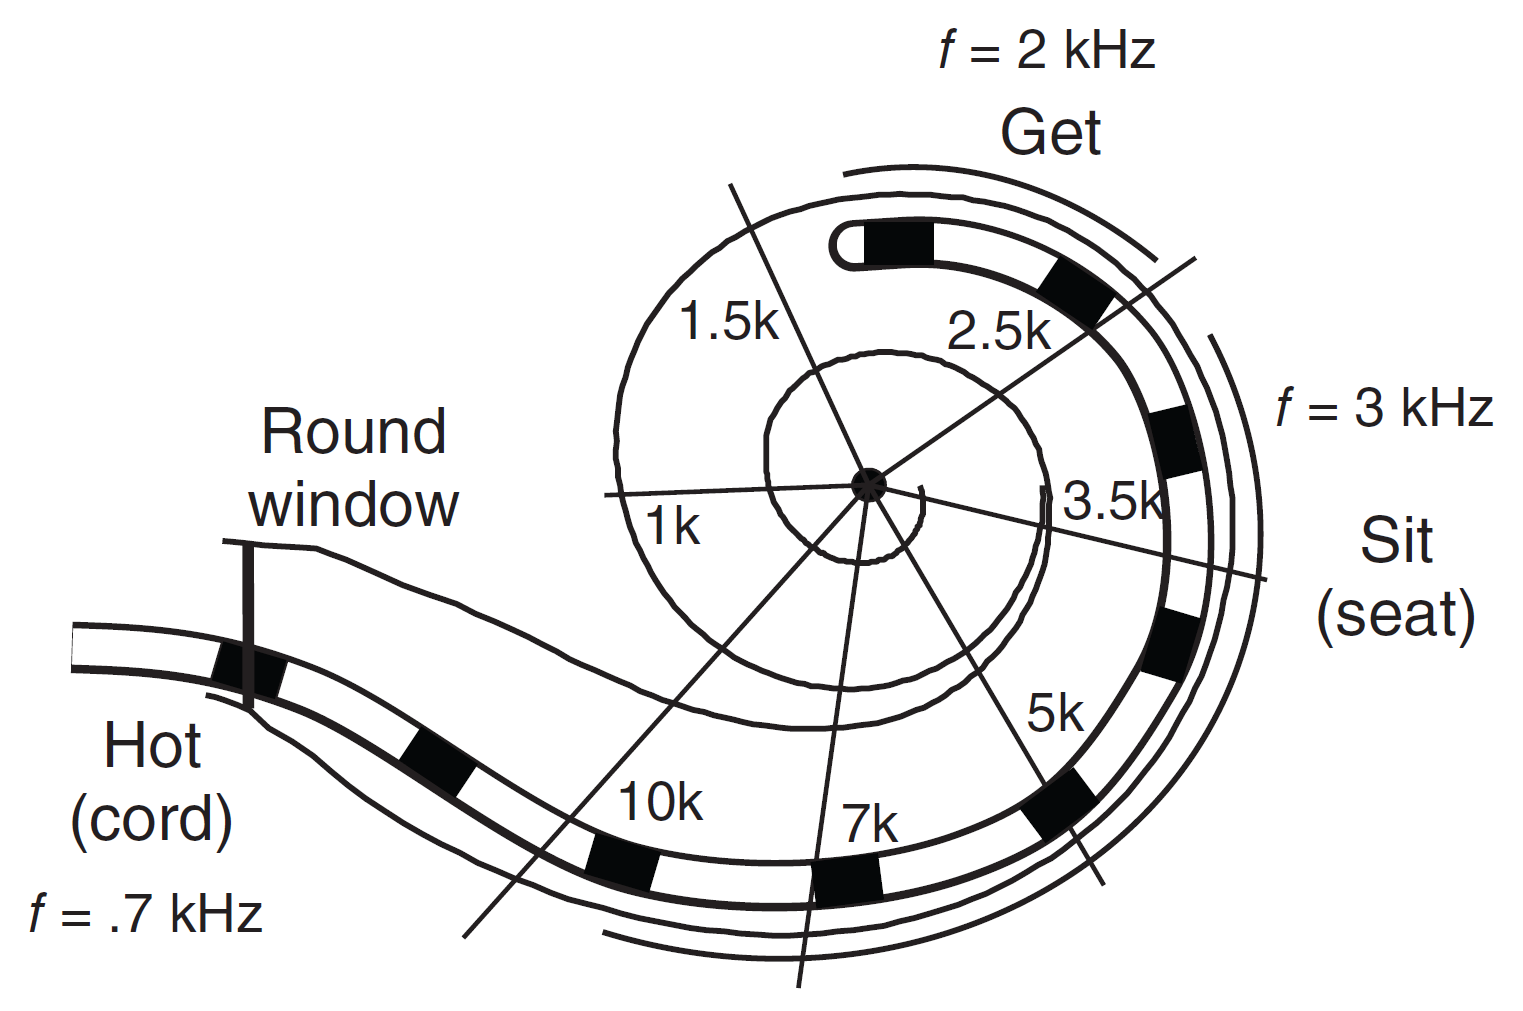
\includegraphics[height=6cm]{Background/pitch_place}
	\caption[Correlation between electrode location and perceived
	frequency]{Correlation between intracochlear electrode location and perceived
	frequency as observed in Rodney Saunders, the first cochlear implant recipient.
	Note the similarities with Figure~\ref{fig:tonotopy}. (Source:
	Clark~\cite{clark2013}. Copyright \textcopyright{} 2013, Macmillan Publishers
	Limited.)}
	\label{fig:pitch_place}
\end{figure}

\subsection{Stimulation Mechanics}

Although the process of charge injection sounds relatively straightforward, the
details of actually implementing such a system are quite complex. Two aspects
that are particularly relevant to this thesis are discussed briefly below.

\subsubsection{Charge Balance}
\label{sect:charge_balance}
% Talk about different stimulation modes and rates, pulse width vs pulses per
% second (Wilson paper),

Metals are \emph{electronic conductors}, i.e. the particles responsible for
carrying charge are electrons; in contrast, biological tissues are
\emph{electrolytic conductors}---the charge carriers are
ions~\cite{webster1998,grimnes2000}. Since metals contain no free ions and the
inner ear fluids have no free electrons, intracochlear electrodes must transduce
an electronic current into an ionic current to effect charge injection across
the electrode-tissue interface. This is accomplished through chemical reactions
at the interface~\cite{webster1998}.

% Talk about water window?
The typical surface reactions for platinum electrodes are listed in
Table~\ref{table:interface_reactions}. At the time of writing, platinum is the
preferred material for use in intracochlear electrodes because its inertness
makes it unlikely to oxidise and dissolve into the \invivo{}
environment~\cite{merrill2005}---a crucial attribute for safe, long-term
electrical stimulation. The chemical stability of the electrode alone is,
however, not a sufficient condition for safety.

\begin{table}
	\centering
	\sffamily
	\small
	
	\caption[Surface reactions at the electrode-tissue interface]{Surface reactions
	at the electrode-tissue interface, in order of increasing potential.
	(Compiled from various sources~\cite{brummer1977,merrill2005}.)}
	\label{table:interface_reactions}
	
	\begin{subtable}[t]{0.8\textwidth}
        \caption{Oxidation reactions.}
        \label{table:interface_reactions_ox}

        \centering
        
        \begin{tabularx}{\textwidth}{p{3.5cm} X}
		\toprule
		\textbf{Reaction}		& \textbf{Equation} \\
		\midrule
		
		Oxygen plating			& \ce{Pt + 2[OH]-} $ \rightleftharpoons $ \ce{PtO + H2O	+ 2e^-} \\
		Oxygen evolution		& \ce{4[OH]^-} $ \rightleftharpoons $ \ce{O2 + 2H2O + 4e^-} \\
		Oxidation of organics	& \ce{CH3CH2OH + 2[OH]^-} $ \rightleftharpoons $ \ce{CH3CHO + 2H2O + 2e^-} \\
		\tableindent\textit{(example)} & \\
		Platinum dissolution 	& \ce{Pt + 4Cl^-} $ \rightleftharpoons $ \ce{[PtCl4]^{2-} + 2e^-} \\
		Chlorine evolution		& \ce{2Cl^-} $ \rightleftharpoons $ \ce{Cl2 + 2e^-} \\
		
		\bottomrule
		\end{tabularx}
		
    \end{subtable}
    
    \vspace{10pt}
    
    \begin{subtable}[t]{0.8\textwidth}
        \caption{Reduction reactions.}
        \label{table:interface_reactions_red}

        \centering
        
        \begin{tabularx}{\textwidth}{p{3.5cm} X}
		\toprule
		\textbf{Reaction}		& \textbf{Equation} \\
		\midrule
		
		Oxygen reduction		& \ce{1/2O2 + H2O} $ \rightleftharpoons $ \ce{H2O2} \\
		Hydrogen plating		& \ce{Pt + H^+ + e^-} $ \rightleftharpoons $ \ce{PtH} \\
		Hydrogen evolution		& \ce{2H^+ + 2e^-} $ \rightleftharpoons $ \ce{H2} \\
		
		\bottomrule
		\end{tabularx}
		
    \end{subtable}
	
\end{table}

Consider electric current that is applied in a single direction, say from the
electrode to the inner ear fluids. With time, this current will deliver a net
charge that favours oxidation reactions, and the products of these reactions
will accumulate and diffuse away from the electrode-tissue interface due to
concentration gradients~\cite{grimnes2000}. These products, such as the
evolution of chlorine gas \invivo{} (Table~\ref{table:interface_reactions_ox}),
may be harmful to the cochlear
tissues~\cite{lilly1955,brummer1977,shepherd1991}.

To prevent such a situation, current is typically delivered as charge-balanced
biphasic pulses~\cite{cogan2008}, an example of which is illustrated in
Figure~\ref{fig:biphasic_pulse}. The first phase of a biphasic input is
responsible for neuronal recruitment~\cite{ranck1975,reilly1998,zeng2004}. The
second phase, which occurs during the refractory period of the stimulated
neurons, serves to neutralise the overall charge and reverse any reactions
induced during the first phase. Most electrical stimulation systems use
cathodic-first pulses because cathodic stimulation produces a higher
depolarisation peak than anodic stimulation~\cite{ranck1975} and therefore
requires less current to reach the threshold for excitation.

\begin{figure}
	\centering
	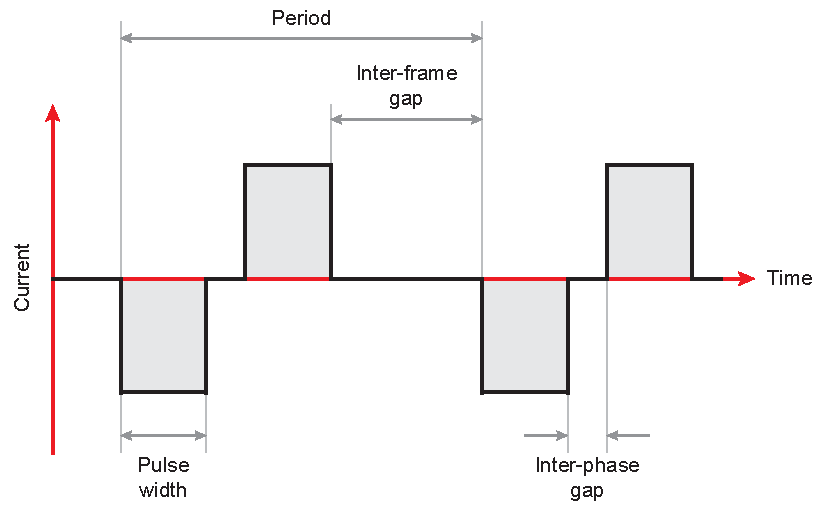
\includegraphics[height=8cm]{Background/biphasic_pulse}
	\caption[Charge-balanced, cathodic-first biphasic pulses]{Charge-balanced,
	cathodic-first biphasic pulses, typically used in electrical stimulation. The
	overall period of a pulse can be divided into subtimings such as the pulse
	width, inter-phase gap, and inter-frame gap as labelled in the diagram. Charge
	delivered during each phase (represented by the shaded areas) should be equal.}
	\label{fig:biphasic_pulse}
\end{figure}

CIs typically use a constant current level for each pulse to simplify the
balancing of electric charge (Figure~\ref{fig:const_current_waveform}). The
phases are usually symmetric (i.e. they have the same amplitude and pulse
width), but it is possible to use asymmetric pulses so long as charge balance is
maintained~\cite{cogan2008}. Constant voltage pulses
(Figure~\ref{fig:const_voltage_waveform}) may also be used, but are not common
in practice. The electric potential at the stimulating electrode varies over
time when constant current pulses are used due to the capacitive effects of the
electric double layer at the
interface~\cite{geddes1972,cobbold1974,grimnes2000}. Care must be taken to
ensure that the total potential does not enter the range that induces
irreversible reactions.

\begin{figure}
	\centering
	\begin{subfigure}[t]{0.6\textwidth}
        \centering
        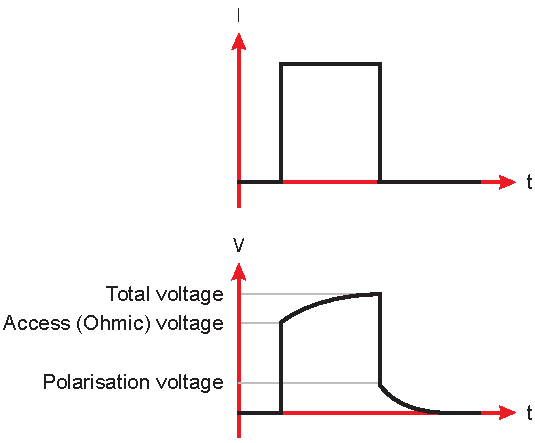
\includegraphics[height=7.2cm]{Background/constant_current}
		\captionsetup{margin={3.65cm,0cm}}
        \caption{ }
        \label{fig:const_current_waveform}
    \end{subfigure}
    ~
    \begin{subfigure}[t]{0.375\textwidth}
        \centering
        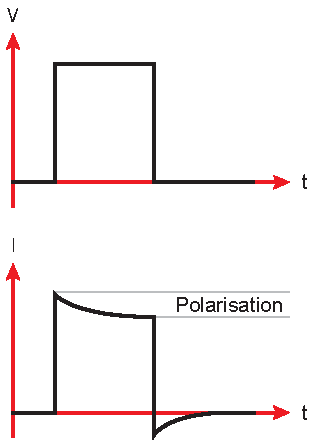
\includegraphics[height=7.2cm]{Background/constant_voltage}
        \captionsetup{margin={-0.05cm,0cm}}
        \caption{ }
        \label{fig:const_voltage_waveform}
    \end{subfigure}
    
	\caption[Constant current versus constant voltage waveforms]{Current and
	voltage waveforms for (a) constant current pulses, and (b) constant voltage
	pulses. Constant current pulses are generally preferred because they make it
	easier to ensure zero net charge injection. The access voltage is the same at
	both the leading and trailing edges of the pulse. (Adapted from
	Webster~\cite{webster1998}.)}
	\label{fig:current_voltage_waveforms}
\end{figure}

\subsubsection{Electrode Configurations}
\label{sect:electrode_configs}

Most CI systems in use today have multiple channels and up to two dozen
independent electrodes~\cite{clark2006}. Cochlear Limited's Contour Advance, for
example, has 22 half-banded platinum contacts along the intracochlear array, a
platinum ball-shaped electrode that is tethered to the implant unit, and the
exposed titanium casing around the stimulator circuitry, which effectively
serves as a plate electrode. Since a source-sink configuration can be set up
between any subset of these electrodes, there are a variety of different
combinations that may be employed~\cite{busby1994}, some of which are
illustrated schematically in Figure~\ref{fig:stim_modes}.

\begin{figure}
	\centering
	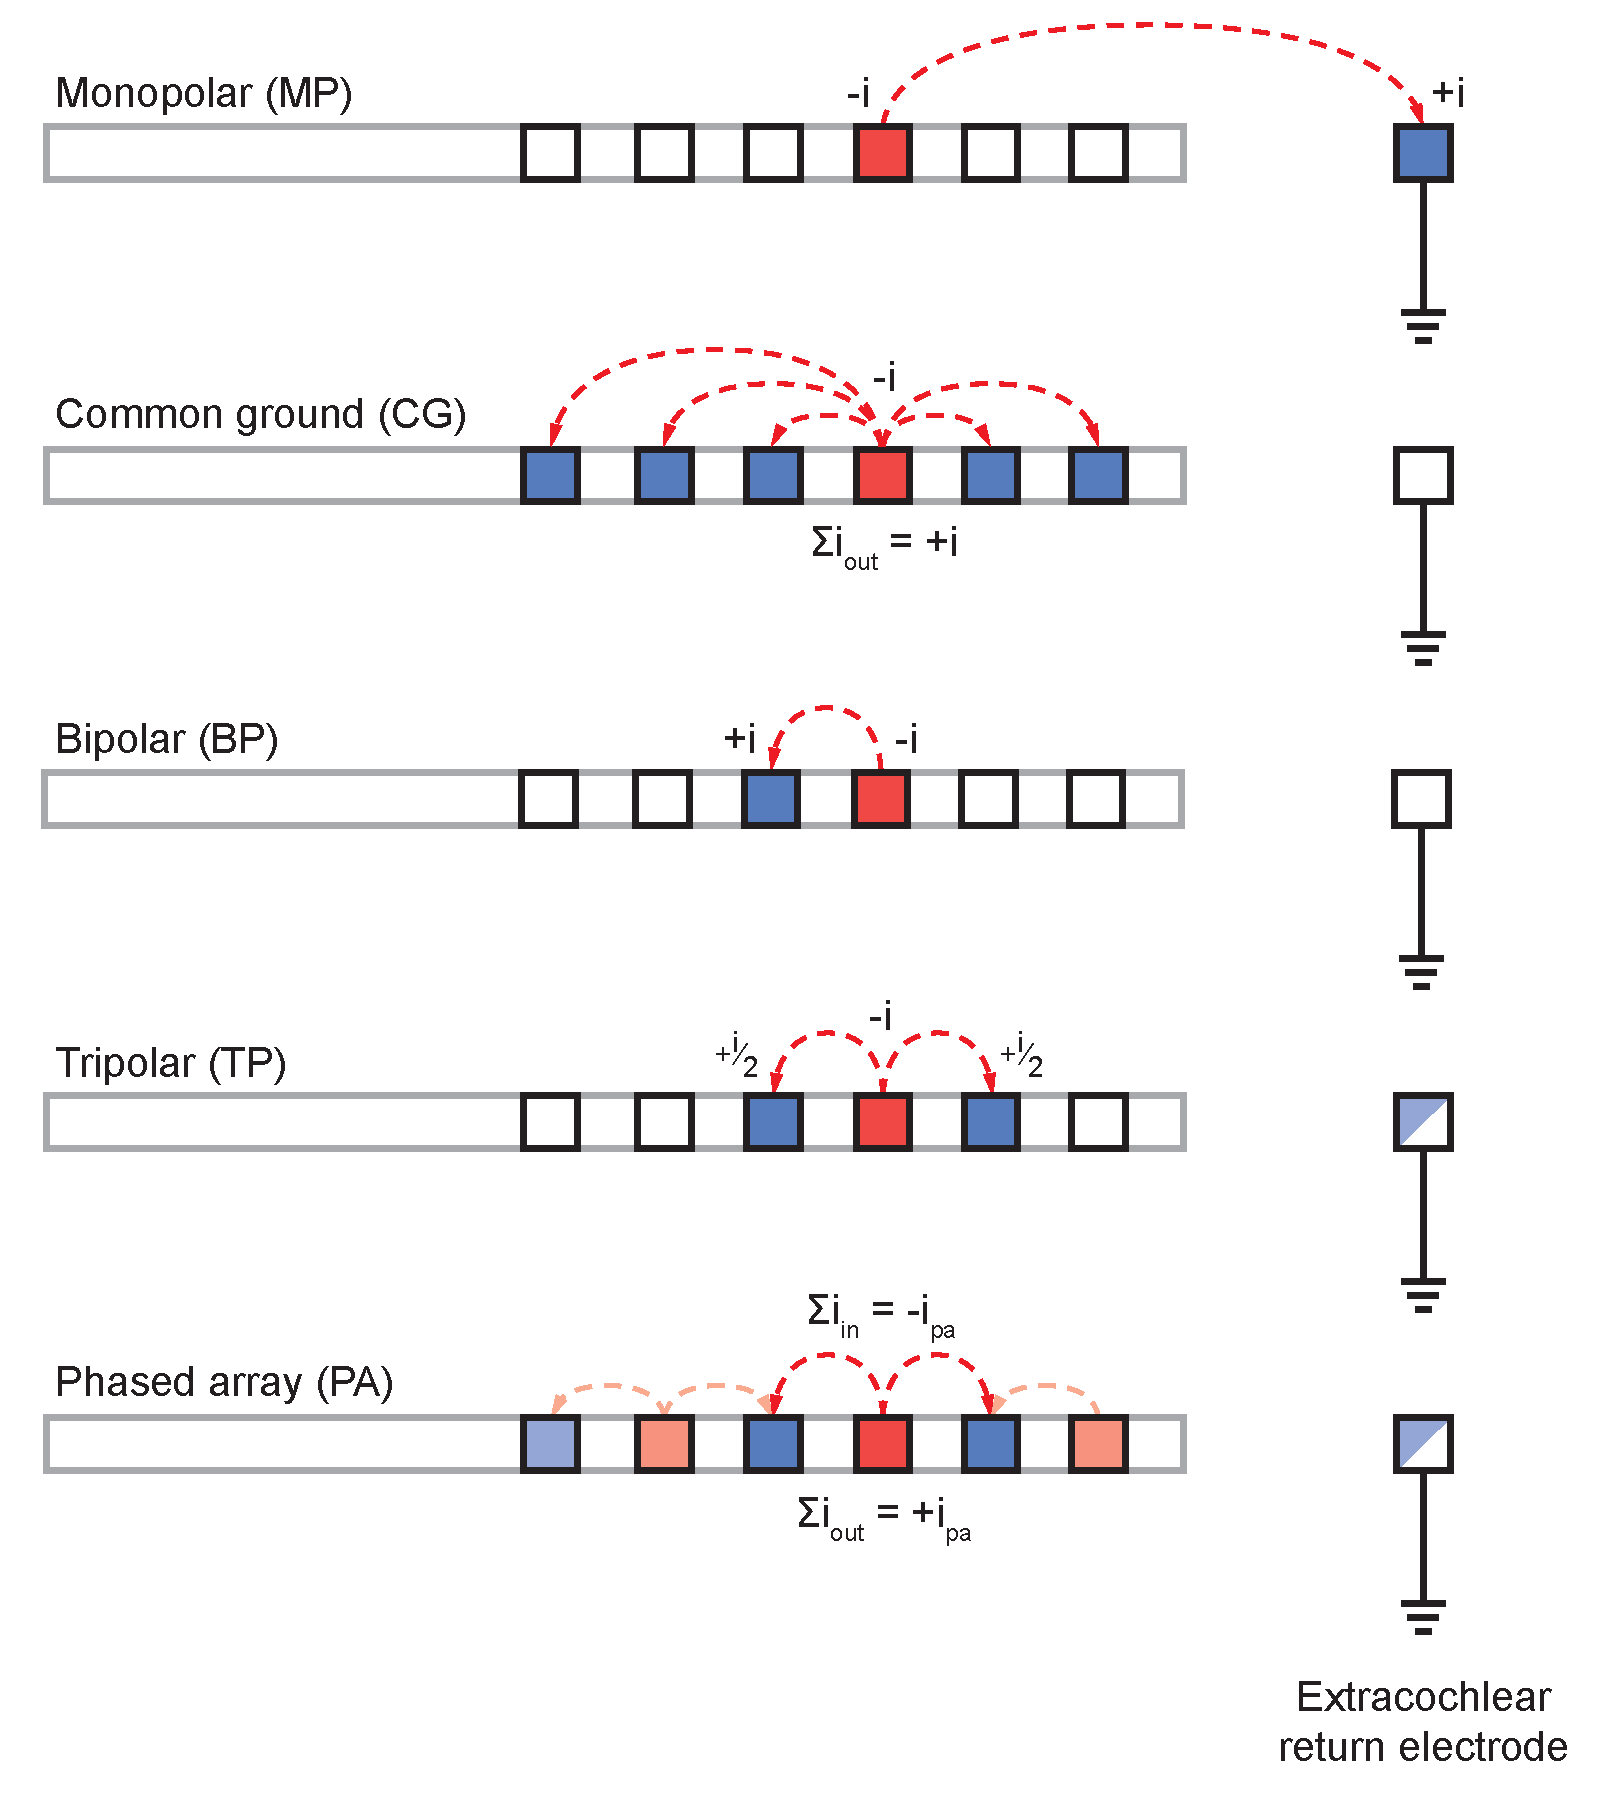
\includegraphics[width=12.8cm]{Background/electrode_config.pdf}
	\caption[Modes of stimulation]{Modes of stimulation for a cochlear implant.
	MP stimulation is the most common mode used in implant recipients. Note that
	the extracochlear electrode may be used in TP and PA stimulation modes.
	Different configurations produce different current paths in the cochlear
	volume, and the resulting perception of sound can differ in many ways.}
	\label{fig:stim_modes}
\end{figure}

\emph{Monopolar} (MP) stimulation is the most common configuration used in
contemporary CIs. Here, current is only injected at one of the intracochlear
electrodes, and returns via the bodily tissues to one or both of the
extracochlear electrodes. This mode of stimulation tends to yield the lowest
thresholds~\cite{busby1994} (i.e. the minimum current level required for the CI
recipient to perceive sound) because the injected current spreads out from the
source electrode, but conversely, the current is also the least
focused~\cite{bonham2008}, stimulating neurons over a relatively wide band of
frequencies in the process~\cite{kral1998,vandenhonert2007}.

Stimulating a narrower band of neurons is an important goal because it enables
finer pitch discrimination in CI recipients~\cite{kral1998,vandenhonert2007}.
One way to achieve this is to use \emph{common ground} (CG) stimulation, where
the non-stimulating electrodes are used together as a single return path instead
of the extracochlear electrode~\cite{busby1994}. In a \emph{bipolar} (BP)
configuration, two intracochlear electrodes are used as the source and the sink.
The two electrodes are typically adjacent, but may also be separated by one or
two pads (known as BP+1 and BP+2, respectively). BP stimulation was often used
during the early phases of multielectrode CI development because, at least in a
homogeneous material, injected current would flow more or less directly between
the two electrodes, limiting the spread of excitation~\cite{black1980,kral1998}.
A variation of BP, called \emph{tripolar} (TP) stimulation, splits the return
path between both adjacent flanking electrodes and, if desired, the
extracochlear electrode, generating a more symmetric field like that of MP
stimulation but with less current spread~\cite{kral1998,busby1994}.
Recent research efforts have looked at \emph{phased array} (PA)
stimulation~\cite{vandenhonert2007,frijns2011,george2014}, also known as
multipolar stimulation in some texts. In this mode, opposing currents are
applied at all electrodes, with weightings based on the inverted transimpedance
matrix along the array to yield a resultant voltage profile that is zero at all
but the stimulating electrode(s)~\cite{vandenhonert2007}.

As with other design decisions, there are costs associated with the use of more
focused stimulation modes. \textit{Ceteris paribus}, the trade-off is higher
power draw when generating auditory percepts at any given level of
loudness~\cite{vandenhonert2007,saba2012}. In addition, there may be no
perceptual benefit in using more focused modes if the residual spiral ganglion
cell bodies in the region of the targeted frequency band have already
degenerated~\cite{pfingst2011}.

\subsection{Efficacy and Unsolved Challenges}

CI stimulation has come a long way since the first recipient was
implanted~\cite{black1980,clark2013}. Clinical reviews, such as those by Nadol
and Eddington~\cite{nadol1988treatment} and Clark~\cite{clark1996}, have shown
significant progress in the restoration of hearing perception. Economic
reports~\cite{economics2006} have also noted their benefit to the wider society
due to flow on effects such as increased productivity and wellbeing in CI
recipients. Indeed, the mere fact that the industry itself exists is a testament
to the success of the CI in fulfilling its mandate.

Nonetheless, there are several scenarios for which CIs can still be
significantly improved. Firstly, noisy environments are commonly encountered in
daily life and present an ongoing challenge for CI recipients because the noise
masks individual sound signals, making it difficult to isolate the desired
source~\cite{stickney2004,gfeller2007}. Secondly, music perception has been
found to be less enjoyable following implantation due to inadequate pitch and
timbre perception~\cite{leal2003,mcdermott2004,sucher2007}. Thirdly, although
the CI is well tuned for English speakers, those who speak tonal languages miss
out on a lot of semantic
information~\cite{ciocca2002,xu2002,wei2004,vandenhonert2007}. Many have called
for or assumed that better speech processing techniques will overcome these
challenges because most of the improvements in patient outcomes have thus far
stemmed from research in that
area~\cite{skinner1994,loizou1998,micco2006,vandenhonert2007}, but despite the
merits of more sophisticated algorithms, updates in speech processing have not
resulted in the desired level of clinical advancement for many years
now~\cite{seligman2004,zeng2008}.

Considering that the mechanism ultimately responsible for auditory nerve
stimulation is the \invivo{} current distribution, it would appear that the
bottleneck of information transfer in CI systems lies with the implanted unit,
specifically with existing designs of the intracochlear electrode
array~\cite{clark2008,clark2013}. Given the difficulties of obtaining and
visualising such information using \invivo{} and \invitro{} experiments alone, a
detailed \insilico{} electroanatomical map of CI induced current flows would be
valuable for furthering our understanding of the cochlea's electrical
behaviour~\cite{spelman1982,girzon1987,suesserman1993,frijns1995,schimpf1998,
micco2006,whiten2007,potratz2010}. An accurate and well-validated model has the
potential to reveal methods for achieving more precise spatial control of the
electric field generated by the CI, as well as other benefits such as lower
power consumption. New intracochlear electrode array designs may also be
virtually prototyped and tested for efficacy before any physical assets are
requested~\cite{zeng2004}, reducing the overall cost of development while
optimising implant design and performance.

% ==============================================================================

\section{Bioelectric Modelling}

\subsection{Expected Physics}
\label{sect:expected_physics}

At a fundamental level, the CI is just like any other system of electrical
interactions. The flow of electric current from the stimulating electrode to the
return electrode and the corresponding fields and fluxes are fully described by
\emph{Maxwell's equations}~\cite{maxwell1865}. They can be written in
differential form as:
\begin{eqnarray}
	\nabla \cdot \vec{E} &=& \frac{\rho}{\epsilon_0}
		\label{eqn:maxwell_1} \\
	\nabla \cdot \vec{B} &=& 0 \phantom{\frac{1}{1}}\\
	\nabla \times \vec{E} &=& -	\frac{\partial \vec{B}}{\partial t} \\
	\nabla \times \vec{B} &=& \mu_{0}\vec{J} +
		\mu_{0}\epsilon_{0}\frac{\partial \vec{E}}{\partial t}
		\label{eqn:maxwell_4}
\end{eqnarray}
where $ \nabla $ is the gradient operator, $ \vec{E} $ is the electric field,
$ \vec{B} $ is the magnetic field, $ \rho $ is electric charge density, $
\vec{J} $ is electric current density, $ \epsilon_{0} $ is the permittivity of
free space, $ \mu_{0} $ is the permeability of free space, and $ t $ is time.
Equations~\ref{eqn:maxwell_1}--\ref{eqn:maxwell_4} are also known as Gauss's
law for electricity, Gauss's law for magnetism, Faraday's law of induction, and
Amp{\`e}re's circuit law with Maxwell's addition, respectively.

In a CI system, these field quantities are determined by three main factors: the
locations of the electrodes, the electric properties of the cochlear tissues,
and the magnitude and shape of the injected current pulse. The current pulse is
under the control of the device itself and is therefore a well-known input
quantity. The other factors are more difficult to quantify, but some insight can
be gained from first principles.

In a homogeneous and isotropic cell with end-plate electrodes, the induced
electric field is uniformly distributed
(Figure~\ref{fig:end_electrodes_uniform}). Consider now a cell that is not
homogeneous, but instead contains a second material of different resistivity to
the first. In this case, the flux lines would exhibit some distortion because
the newly introduced material changes the shape of the electric
field~\cite{baker1989}, as shown in Figure~\ref{fig:end_electrodes_distorted}.
Relatively conductive tissues tend to funnel current flow, while those that are
relatively insulating are avoided as the current seeks out the path of least
resistance. The larger the difference in resistivity between the two materials,
the more distortion that can be expected.

\begin{figure}[p]
	\centering
	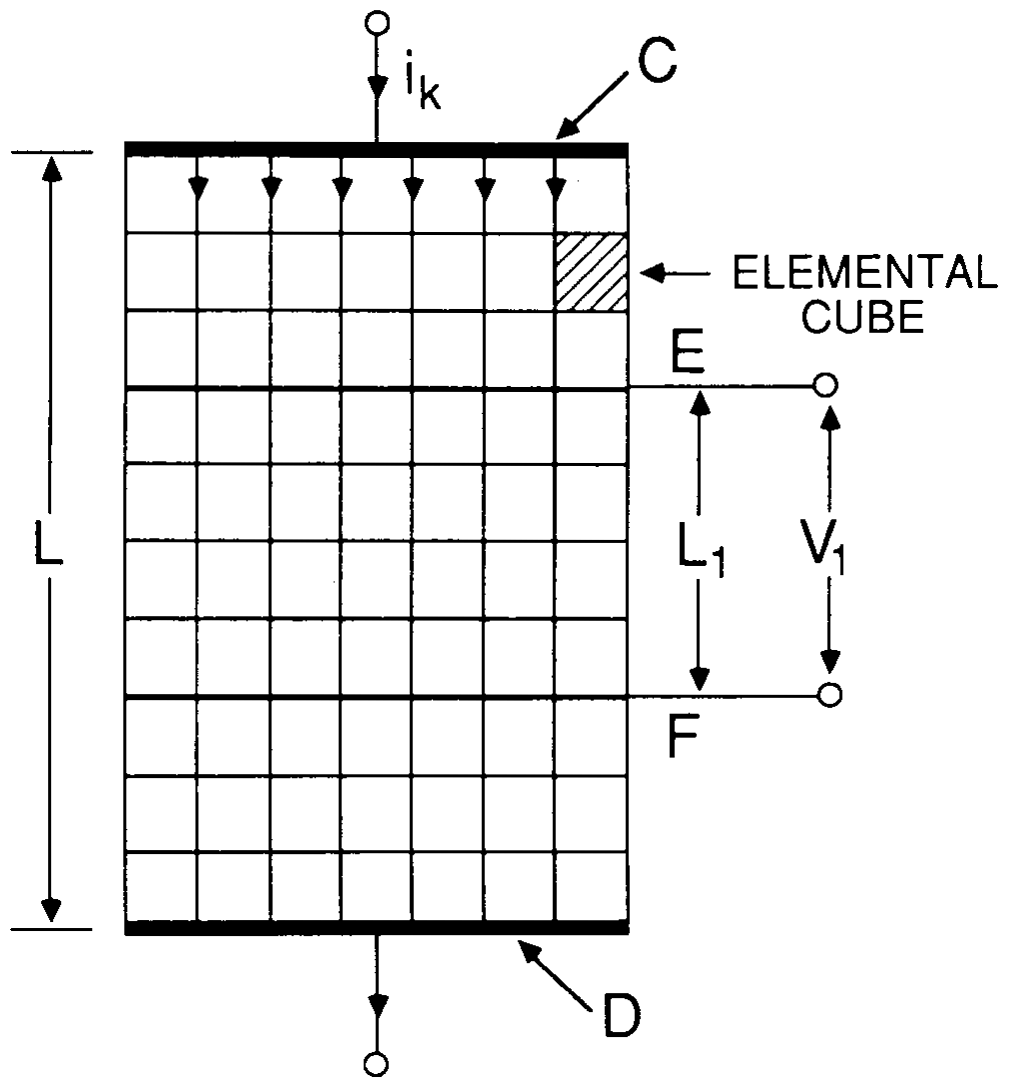
\includegraphics[height=5.6cm]{Background/end_electrodes_uniform}
	\caption[Uniform flux lines in a homogeneous isotropic cell]{Uniform flux lines
	in a homogeneous isotropic cell. (Source: Baker~\cite{baker1989}. Copyright
	\textcopyright{} 1989, IEEE.)}
	\label{fig:end_electrodes_uniform}
\end{figure}

\begin{figure}[p]
	\centering
	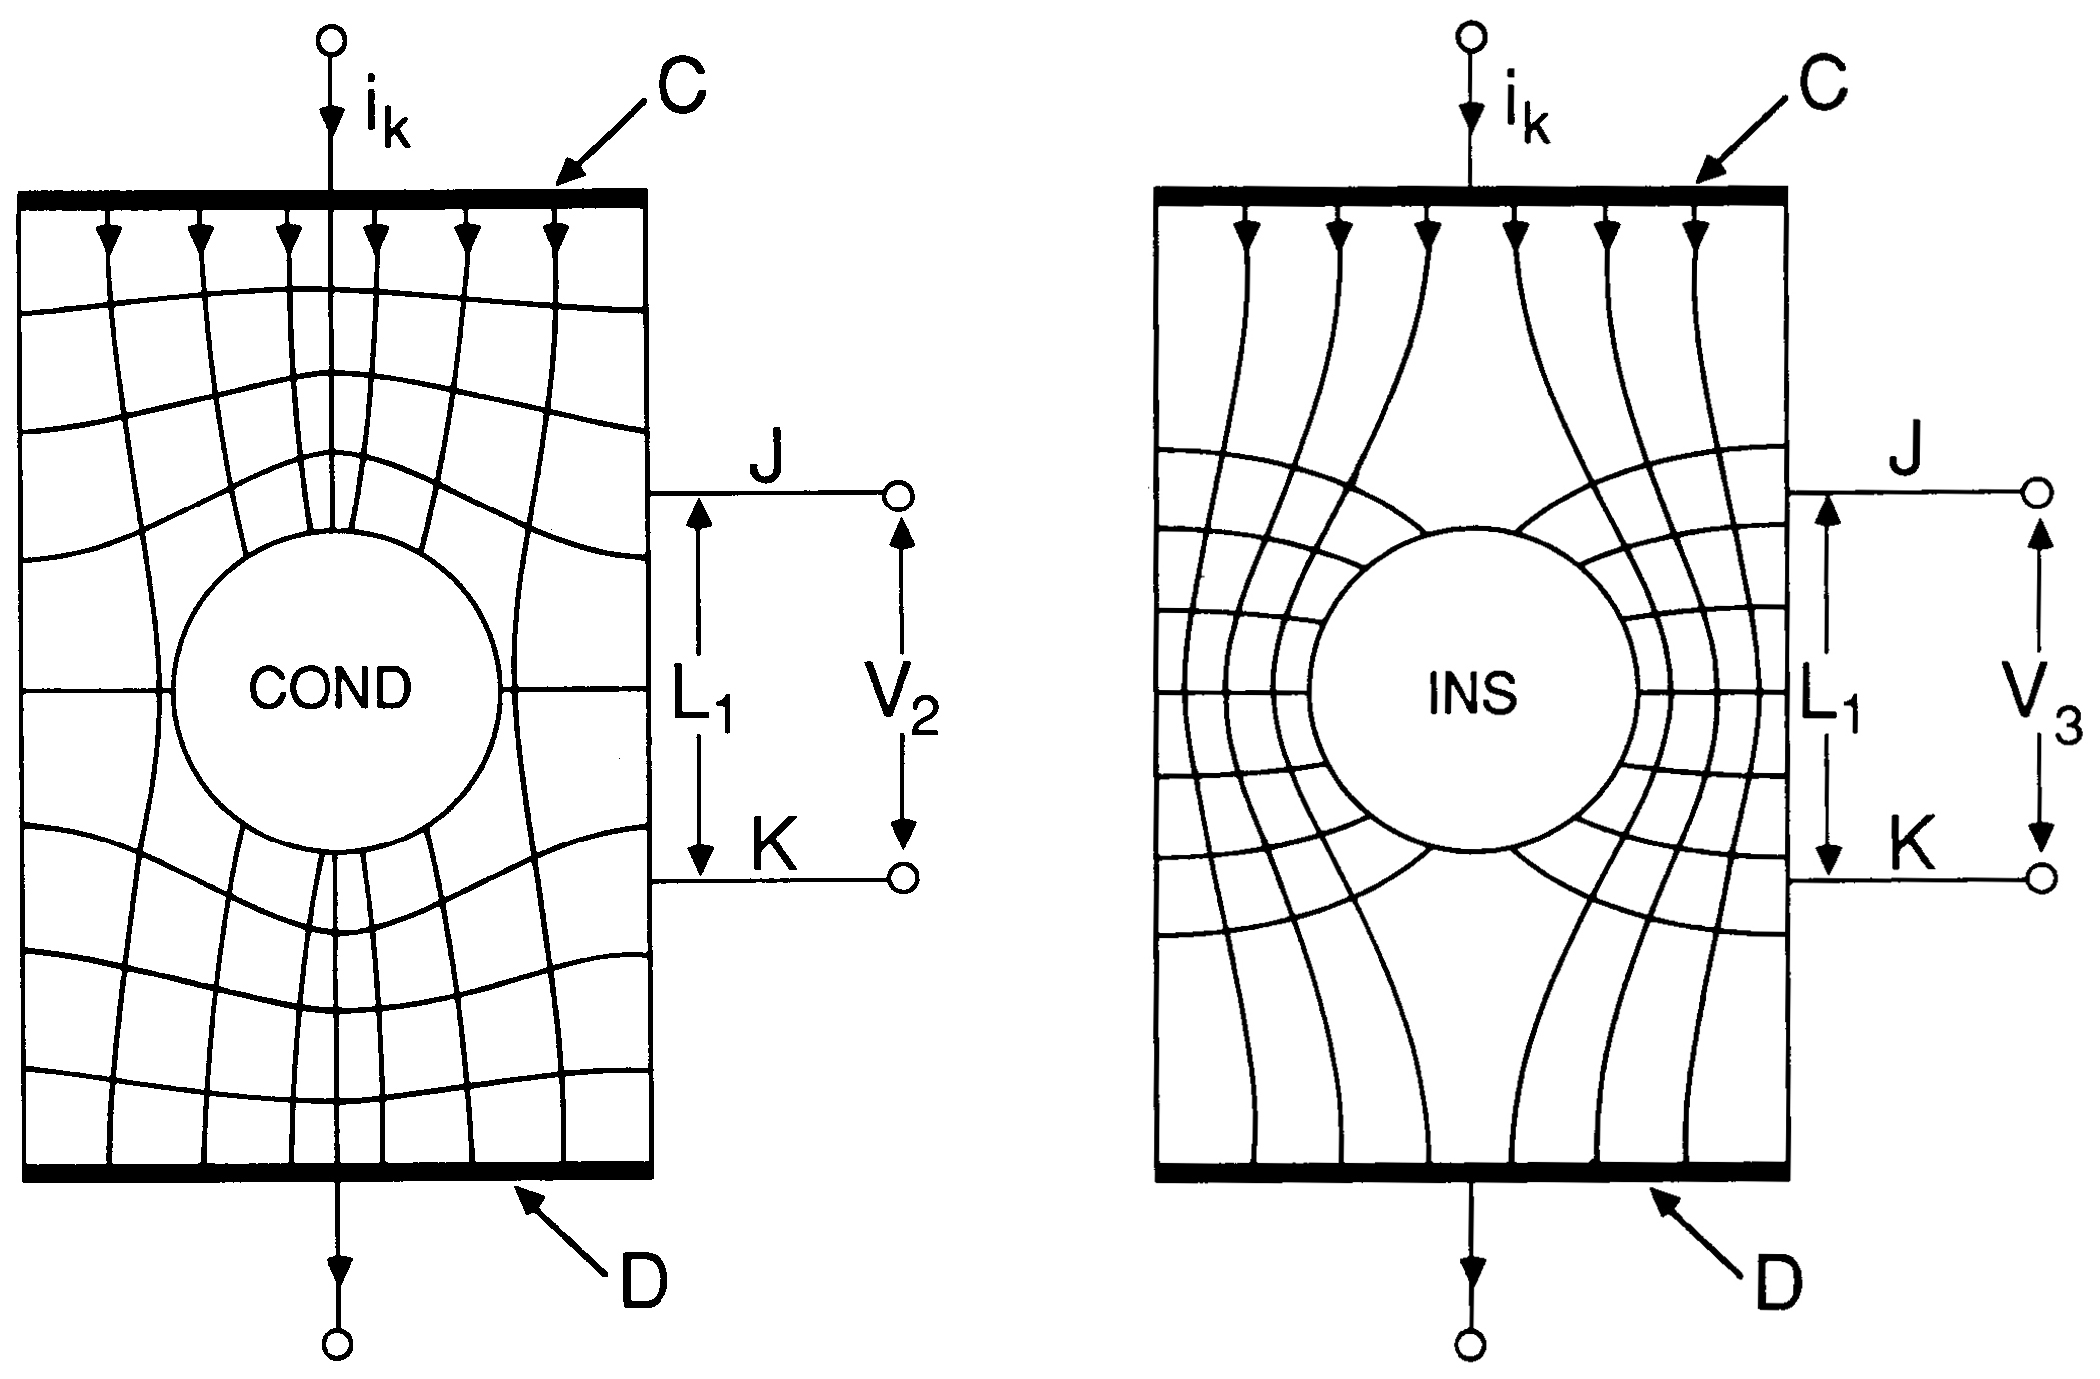
\includegraphics[height=5.6cm]{Background/cond_ins}
	\caption[Distortion of flux lines in the presence of a conductor
	or an insulator]{Distortion of flux lines in the presence of a conductor
	(left) or an insulator (right) when using end-plate electrodes. (Source:
	Baker~\cite{baker1989}. Copyright \textcopyright{} 1989, IEEE.)}
	\label{fig:end_electrodes_distorted}
\end{figure}

\begin{figure}[p]
	\centering
	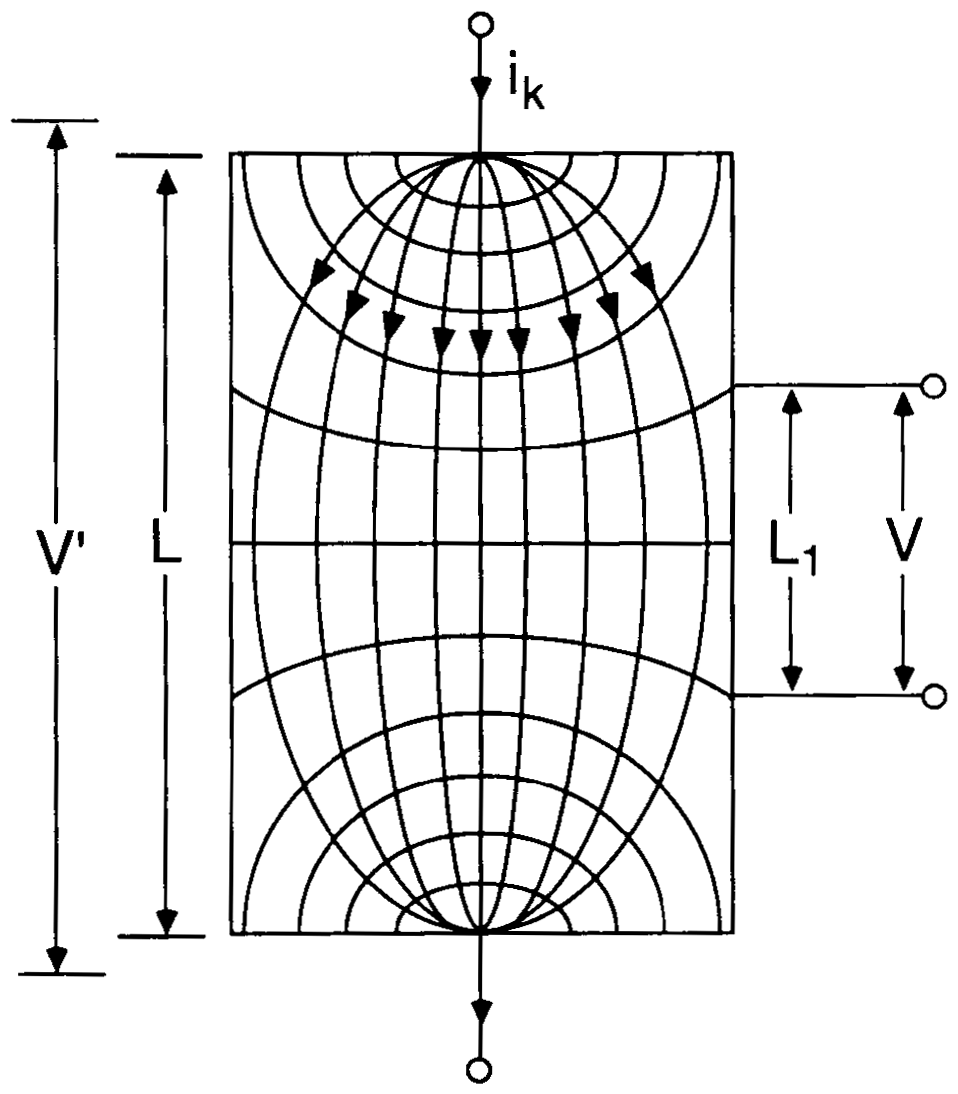
\includegraphics[height=5.6cm]{Background/small_electrodes_flux}
	\caption[Flux lines with small electrodes]{Flux lines with small electrodes.
	Note the non-uniform shape of the current density distribution. (Source:
	Baker~\cite{baker1989}. Copyright \textcopyright{} 1989, IEEE.)}
	\label{fig:small_electrodes_flux}
\end{figure}

Consider again the homogeneous cell, but this time with the end-plate electrodes
replaced by much smaller ones, as per Figure~\ref{fig:small_electrodes_flux}).
Again, the flux lines would deviate from uniformity, but here they would take on
a different pattern, spreading out from the current source through the medium
before reconverging at the sink. Any changes in resistivity that are introduced
in this case would have more impact on the current paths if they are located
near the small electrodes, since this is where the current density is
highest~\cite{baker1989}.

The simulations in this thesis are expected to adhere to the same physics and
thus exhibit both of these patterns. Unlike these simplistic theoretical
examples though, the cochlea consists of many tissues and its three-dimensional
geometry is complex, so the field patterns are not intuitive. Nevertheless, the
current paths will be determined by the anatomical structures as a function of
their material properties, which span a wide range due to large differences in
tissue morphology, and their proximity to the stimulating electrode, which is
small relative to the volume of the cochlea. Note that the cochlear models
themselves are in turn small relative to the entire head, so the reconvergence
of flux lines at the return electrode (as depicted in
Figure~\ref{fig:small_electrodes_flux}) is not expected to occur within the
modelled domain under MP stimulation.

\subsection{Numerical Methods}
\label{sect:numerical_methods}

\subsubsection{Rationale for Computational Modelling}
\label{sect:rationale_for_modelling}

There are several ways these complex electric field patterns could be
characterised in a spatial sense. A rudimentary method would be to measure the
electric potential at numerous points throughout the cochlea of a CI recipient
and then correlate these data with the Cartesian location of each sample to
generate an electroanatomical map~\cite{kral1998}. Such direct measurements
could provide very realistic results since the biological aspects of the system
are inherently accounted for. However, the need to physically intrude into the
cochlear tissues makes this impractical for both \invivo{} and \invitro{}
studies, as noted in \S\ref{sect:knowledge_dev}.

An alternative approach would be to take measurements at fewer, more accessible
locations, and make assumptions about the behaviour of the electric field at
points that are not directly measured~\cite{kral1998}. That is, in essence, the
modelling process, which has become a preferred method of investigation for CI
research. Early efforts used \emph{lumped-element models} (LEMs), which
attempted to represent the electric response of the implanted cochlea as an
equivalent electric circuit. Key locations, such as the position of the
stimulating and measuring electrodes, were connected by a network of electric
circuit components (typically resistors), with each component representing the
response of one or more of the biological tissues along a presumed current
pathway between the connected nodes.

However, a quick comparison of the published LEMs reveals a major flaw in this
approach: since the true shape of the cochlea is ignored, the selection of
electrical elements and connections in these circuits is arbitrary, leading to a
multitude of circuit representations for the same electroanatomical system (see
\S\ref{sect:lumped_element_models}). The models were sufficient insofar as each
LEM was only related back to the corresponding experimental measurements to
yield bulk impedances between two points in that circuit. LEMs are therefore
useful for global insights into CI
stimulation~\cite{machado1996,briaire2000mesh}, but better spatial
representation is required for more generally applicable results.
Indeed, von \bekesy{} noted in his pioneering study that the use of more
elements in the network would provide a closer approximation of the \invivo{}
situation~\cite{vonbekesy1951}.

The development of integrated circuits in the 1970s was a significant milestone
for modelling research because it enabled the development of numerical solution
methods that were computationally intense. Although these numerical methods were
originally developed for structural mechanics, they were later applied to other
types of physics by discretising the appropriate governing equations; in the
case of electromagnetic simulations, these are the aforementioned Maxwell's
equations. Sustained increases in processing power, driven by advances in
microprocessor architectures and manufacturing processes, meant that by the
mid-1980s, a new class of electroanatomical model, based on numerical analysis,
had become viable~\cite{bondeson2005}. These models are generally referred to as
\emph{volume conduction models} (VCMs) because the geometry of the modelled
domain is based on the true three-dimensional (3D) shape of the physical system.
VCMs of the implanted cochlea are reviewed in
\S\ref{sect:volume_conduction_models}.

Numerical methods for bioelectric volume conduction problems have been reviewed
by several
authors~\cite{cendes1989,miller1990,schimpf1998,bondeson2005,johnson2006}. The
main differences between the mathematical formulations of the three most popular
approaches---the \emph{finite difference method} (FDM), the
\emph{finite element method} (FEM), and the \emph{boundary element method}
(BEM)---are summarised below.

\subsubsection{Discretisation and the Finite Difference Method}

All three methods involve approximating the continuous domain with a finite
number of subspaces---a process known as \emph{discretisation} or \emph{mesh
generation}~\cite{reddy1993}. The FDM is the most traditional of the three
approaches and uses the differential form of Maxwell's equations. Under the FDM,
the continuous domain is discretised into a uniform orthogonal grid to yield a
pointwise approximation~\cite{schimpf1998}. At each point, the derivatives are
expressed algebraically as differences between adjacent points in the finite
difference grid. These reference the material properties representing the
electric behaviour of the tissue at that point (namely conductivity and
permittivity). The whole system is then evaluated by recombining the equations
into a global matrix using continuity conditions and solving for the unknown
dependent variable (i.e. the electric potential) at each node using a set of
constraints (namely the \emph{electrical loads} and \emph{boundary
conditions})~\cite{bondeson2005}. The numerical estimate converges to the exact
solution as more subspaces are used; for the FDM, this requires a denser point
cloud.

The FDM is quite simple to implement and compute, making it a good candidate for
time-domain simulations~\cite{bondeson2005}. It is well suited to modelling
devices with man-made geometries and engineering materials, especially those
with straight edges such as cantilever beams. However, geometries that are not
aligned with the grid will suffer from inaccuracies due to the staircase effect
(see Figure~\ref{fig:mesh_comparison}). This means it is unable to accurately
represent the complex organic shapes encountered in anatomical structures, and
faces difficulties imposing certain boundary conditions~\cite{johnson2006}. In
addition, a relatively large number of equations must be solved to achieve a
certain level of accuracy because discretisation using a uniform grid must
account for the finest features of the geometry and the steepest concentrations
in the electric field.

\begin{figure}
    \centering

    \begin{subfigure}[t]{0.5\textwidth}
        \centering
        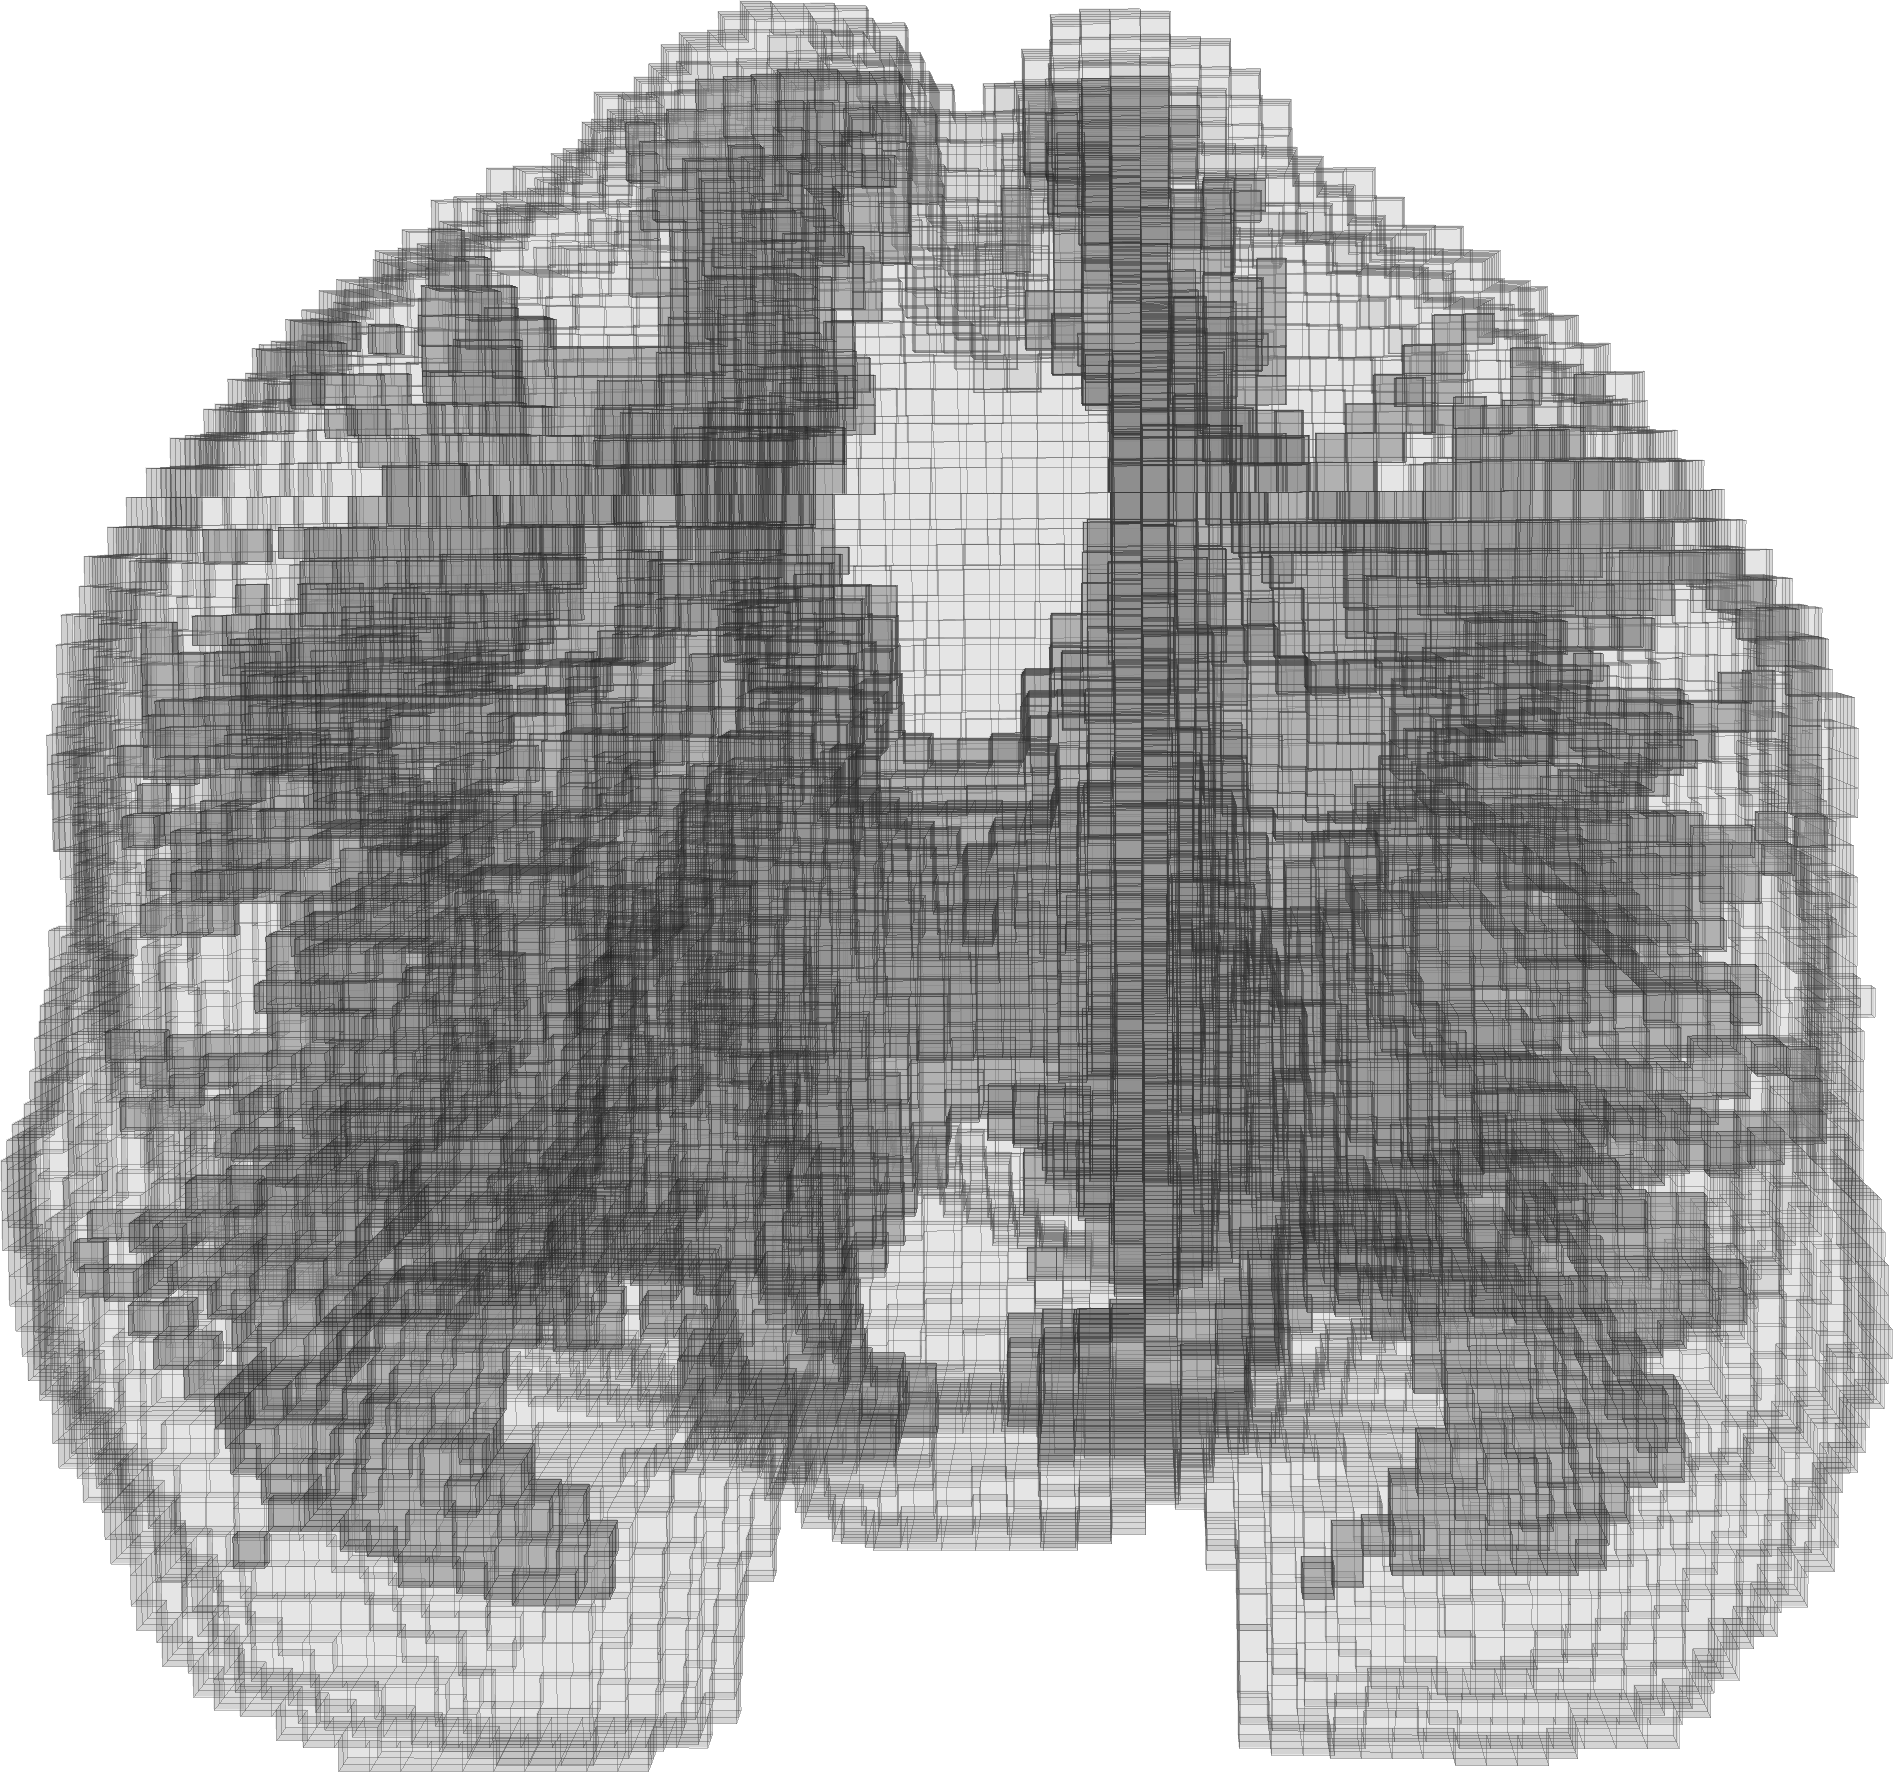
\includegraphics[width=6.5cm]{Background/mesh_grid}
        \caption{ }
        \label{fig:mesh_grid}
    \end{subfigure}%
	\begin{subfigure}[t]{0.5\textwidth}
        \centering
        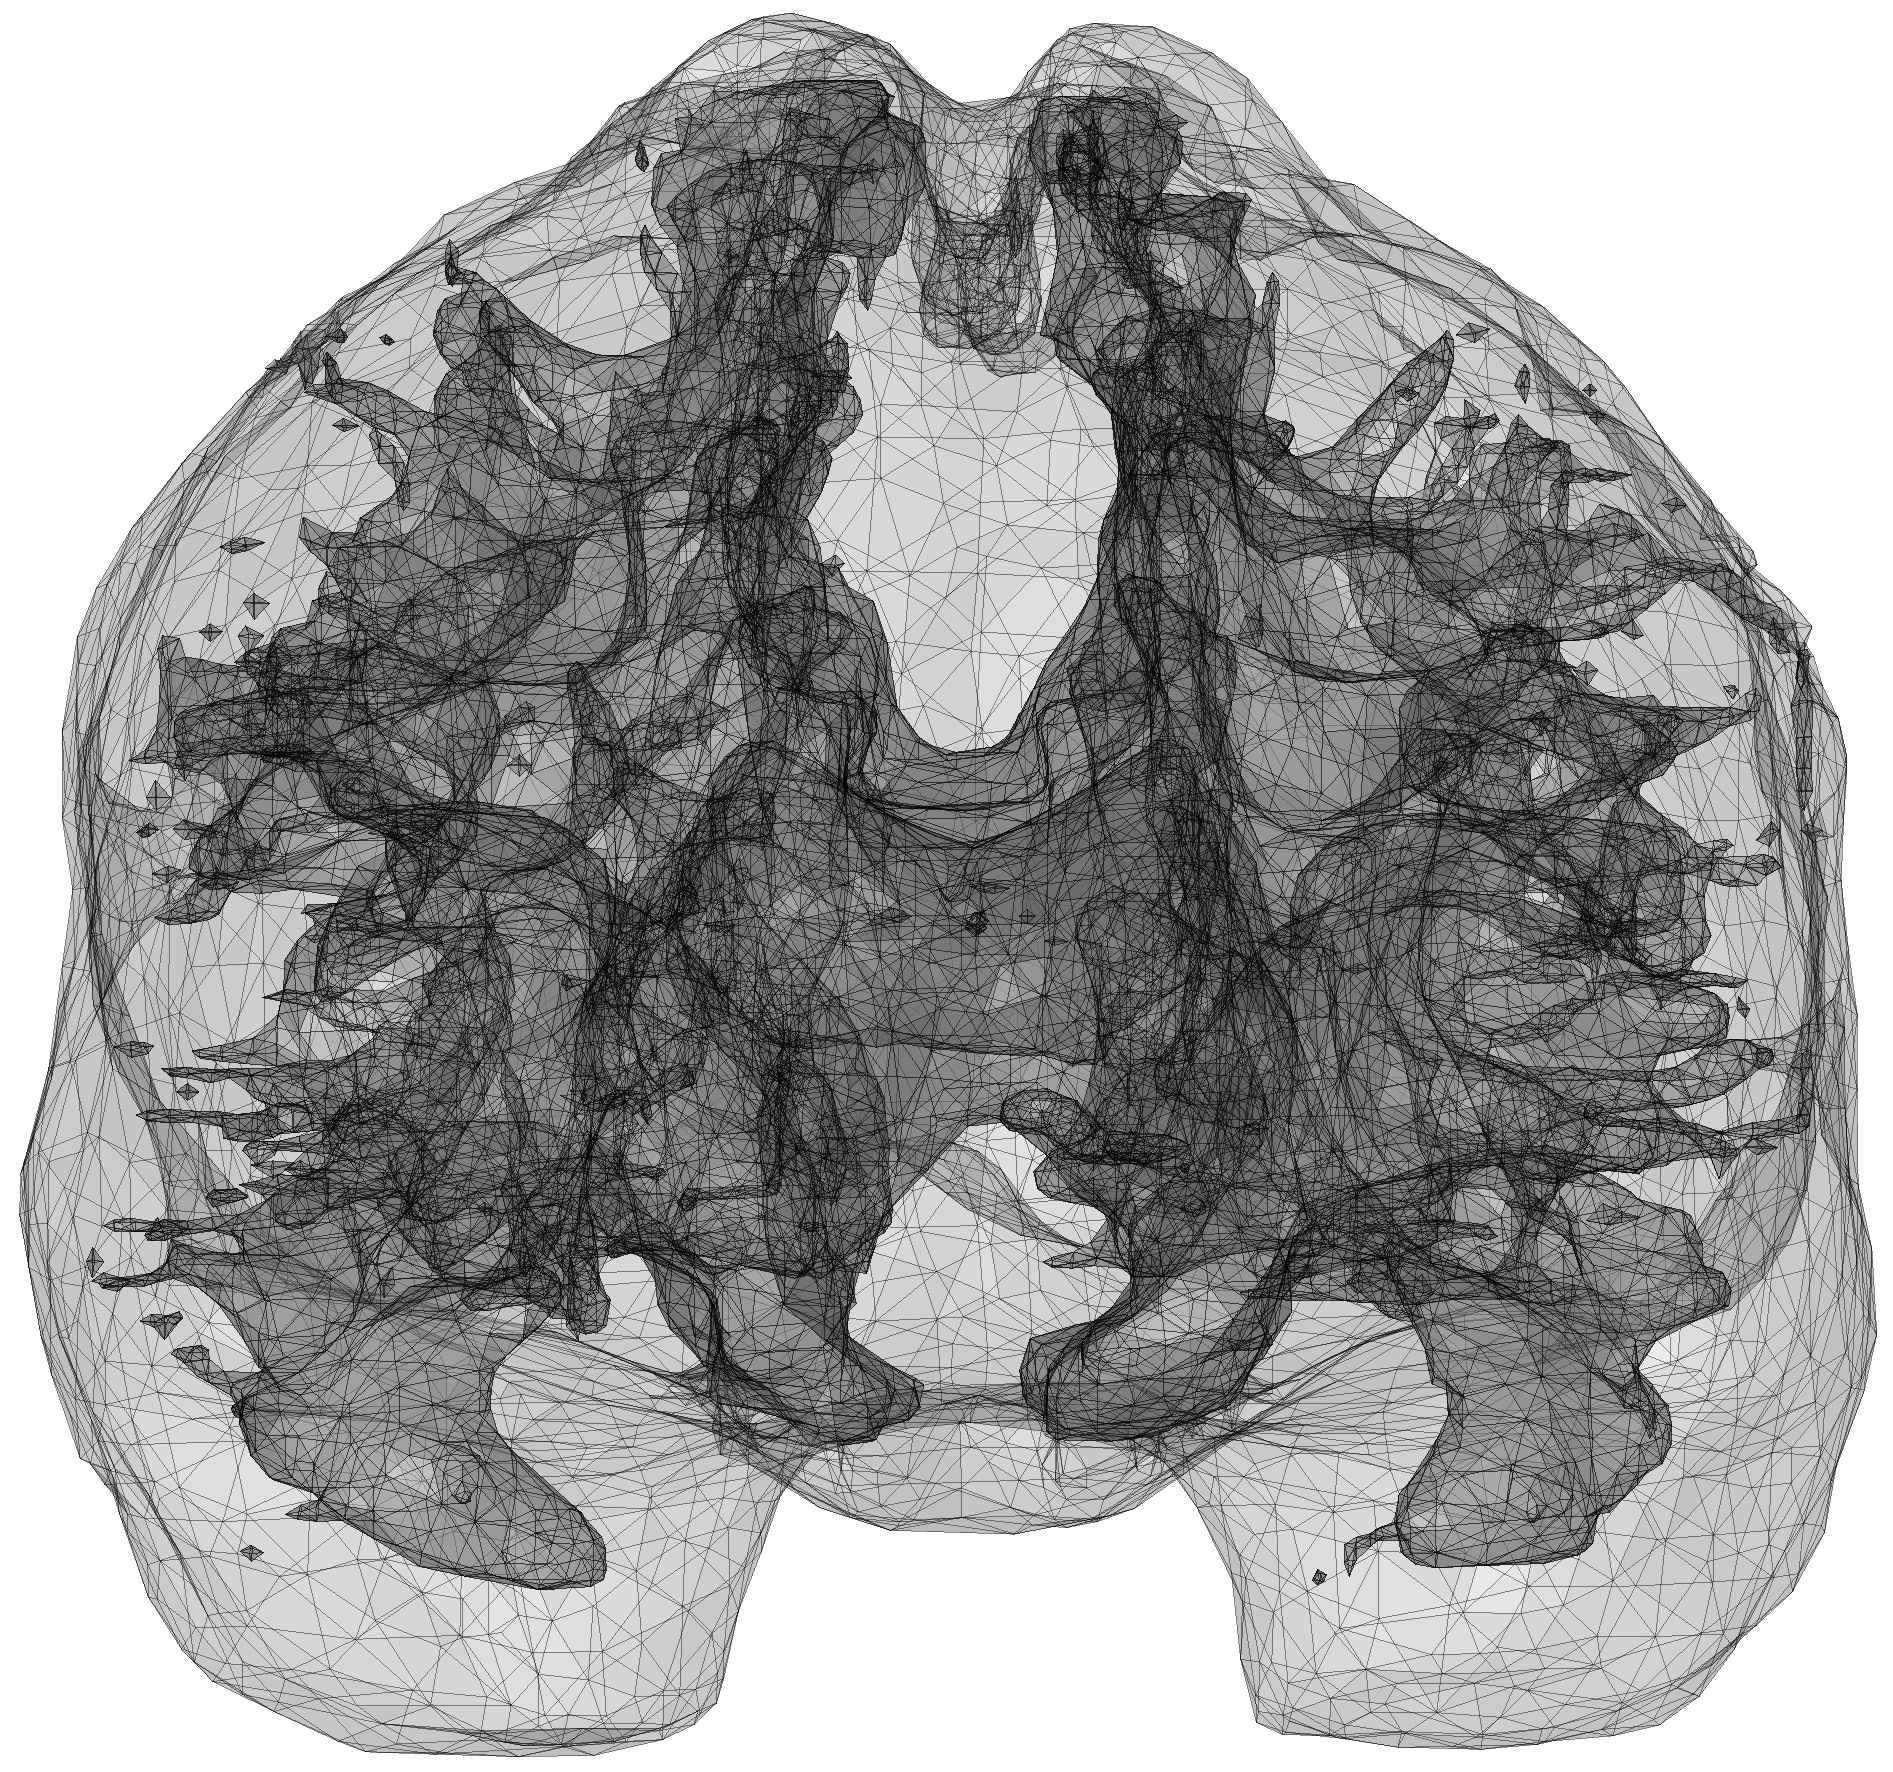
\includegraphics[width=6.5cm]{Background/mesh_free}
        \caption{ }
        \label{fig:mesh_free}
    \end{subfigure}
    
	\caption[Comparison of FDM and FEM meshes]{Comparison of FDM and FEM meshes for
	the brain of HEATHER~\cite{tran2015}. (a) A finite difference mesh exhibits an
	obvious staircase effect. (b) A finite element mesh can produce smoother and
	more realistic boundaries with fewer elements.}
	\label{fig:mesh_comparison}
\end{figure}

\subsubsection{The Finite Element Method}

Generally speaking, the FEM is the most preferred numerical method in
engineering simulations. The main reason for this is its ability to handle
complex geometries~\cite{bondeson2005}. As with the FDM, FEM solvers use
Maxwell's equations in differential form. The difference is that in the FEM, the
continuous domain is discretised into an unstructured mesh.

Instead of using a uniform grid, the points (termed \emph{nodes}) are connected
to form small, discrete regions (\emph{elements}), which have a geometrically
simple (but not necessarily regular nor uniform) shape. Some typical elements
are shown in Figure~\ref{fig:element_types}. In an unstructured mesh, the
distribution of nodes can be non-uniform and non-orthogonal, allowing for a much
smoother representation of curved geometries (cf.
Figure~\ref{fig:mesh_comparison}). This flexible node arrangement also means
that the mesh can be refined locally to improve the accuracy of the solution
around fine geometrical details or regions with steep field gradients without
resorting to a high mesh density throughout the entire domain.

\begin{figure}
	\centering
	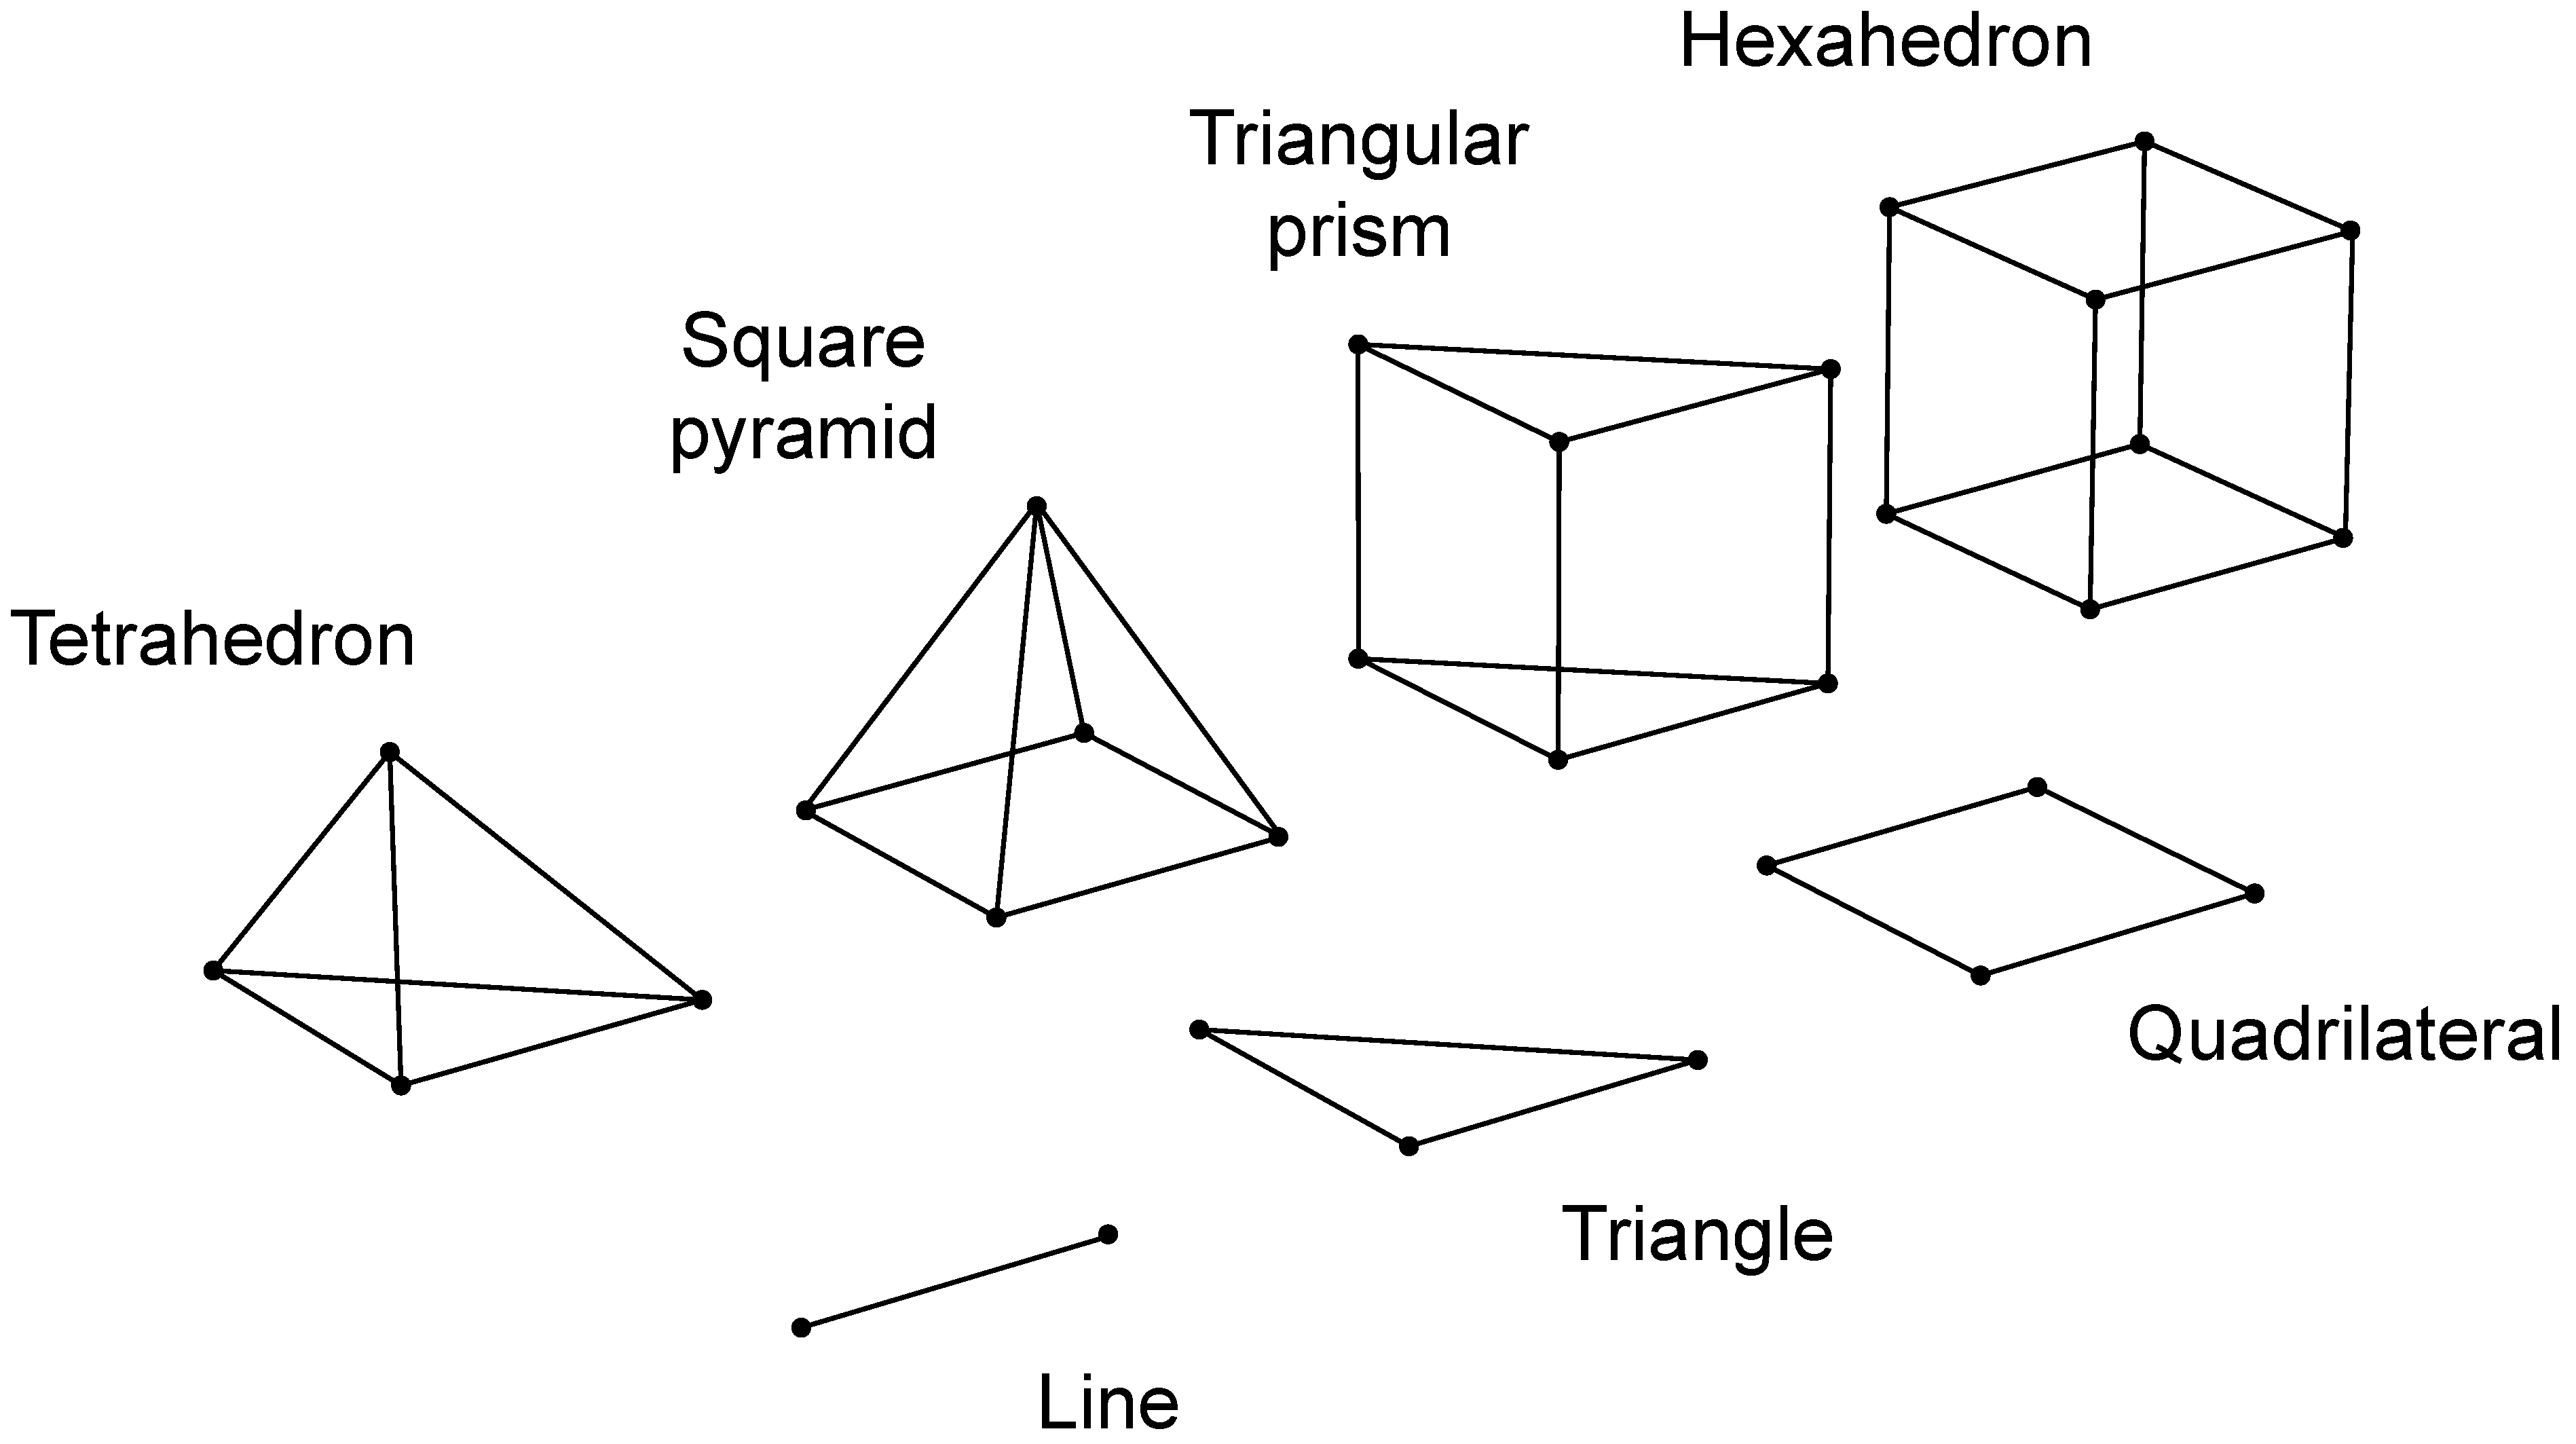
\includegraphics[height=6.2cm]{Background/element_types}
	\caption[Linear finite elements by shape]{Linear finite elements by shape.
	Nodes are shown at each vertex. Quadratically interpolated elements also
	possess mid-side nodes. The final appearance of each element in the mesh is
	typically less regular than those shown here because the elements must conform
	to the geometry of the continuous domain without becoming excessively skewed.
	For 3D problems, the BEM uses planar elements, while the FEM uses volumetric
	elements. (Image adapted from Bondeson~\cite{bondeson2005}. Copyright
	\textcopyright{} 2005, Springer-Verlag.)}
	\label{fig:element_types}
\end{figure}

The formulation of the FEM requires that the change of the dependent variable in
space be defined within each element. This role is fulfilled by an interpolation
function, also known as a \emph{shape function}, which is usually a low order
polynomial defined relative to the values at the nodes of the element. FEM
results can thus also be refined by increasing the order of this shape function.
Because the dependent variable is defined within each element and the global
solution is found by evaluating these with reference to the loads and boundary
conditions, the FEM solution is often described as a piecewise
approximation~\cite{schimpf1998}.

% For all three methods, refinement can be achieved by using smaller subspaces.
% FEM and BEM results can also be refined by using higher order interpolation
% functions, and/or optimising the spatial distribution of the nodes.

\subsubsection{The Boundary Element Method}

The BEM (also known as the \emph{method of moments}) takes a slightly different
approach to the other two methods. In a BEM formulation, the entire volume is
split into compartments by material, and as its name suggests, only the
boundaries between compartments are discretised (using (n--1)-dimensional
elements). However, there are restrictions on the types of geometries that can
be solved. To avoid ambiguity from the dimensional reduction, all compartments
must form closed surfaces and they cannot intersect each other---i.e. they must be
completely nested or completely independent. The material properties assigned to
each compartment must also be constant within the bounding surfaces. These
attributes make the BEM well suited to models that are \emph{homogeneous} (one
material only) and \emph{isotropic} (identical properties in all directions),
for \emph{heterogeneous} models containing only a few materials with similar
properties, and for unbounded problems~\cite{katsikadelis2002}.

Also note that unlike the other two methods, the BEM employs Maxwell's equations
in integral form. The integrand is often decomposed into a singular part, which
has an analytical solution, and a regular part, which is solved numerically.
The analytical component can be an issue for certain classes of problems.

\subsection{Neural Excitation}
\label{sect:neural_excitation}

Calculating the electric field is only one part of the bioelectric problem. For
CI (and other types of electrical) stimulation, it is also of interest to gauge
the consequences of the generated electric field on the excitable tissues, in
this case, the auditory nerves.

\subsubsection{Response of the Neural Membrane}

Like other electrically excitable tissues, the cell membranes of the auditory
nerves contain voltage-gated ion channels (e.g. for \ce{Na^+} influx or \ce{K^+}
efflux) in addition to non-gated channels (e.g. for \ce{Cl^-})~\cite{brown2001}.
The distribution of ion species across the membrane is typically uneven, with
more negative charge inside the cell compared to the outside. This potential
difference, known as the \emph{resting membrane potential}, is on the order of $
-70 $ to $ -90 $ mV, and is maintained by the normal metabolic activity of the
cell. If the ionic permeability of the cell membrane is changed, a local
potential can develop. The cell membrane becomes \emph{depolarised} when the
potential becomes more positive, for example, when there is an influx of
cations; conversely a more negative potential causes it to become
\emph{hyperpolarised}.

Only depolarisation can trigger an action potential~\cite{reilly1998}.
Experiments by Hodgkin and Huxley with unmyelinated squid
axons~\cite{hodgkin1952} and Frankenhaeuser and Huxley with myelinated toad
axons~\cite{frankenhaeuser1964} revealed the ionic mechanisms responsible for
action potential generation. When the electric potential in one region of the
membrane is depolarised to the cell's threshold level, the permeability of the
cell membrane to \ce{Na^+} increases, leading to an influx of \ce{Na^+} which
then further depolarises the cell~\cite{brown2001}. This positive feedback
mechanism quickly reverses the membrane potential in that region, as shown in
Figure~\ref{fig:depolarisation_wavefront}, and the subsequent transfer of charge
from adjacent regions of the membrane causes the depolarisation to propagate. It
is this self-propagating neural impulse that allows signals to be relayed to the
brain. Other voltage-gated channels open after the \ce{Na^+} channels, allowing
\ce{K^+} ions to leave the neuron and restore the resting membrane potential.
The intracellular balance of cations is maintained via sodium-potassium pumps,
which actively transport \ce{Na^+} and \ce{K^+} ions through the membrane
against the concentration gradient.

\begin{figure}
	\centering
	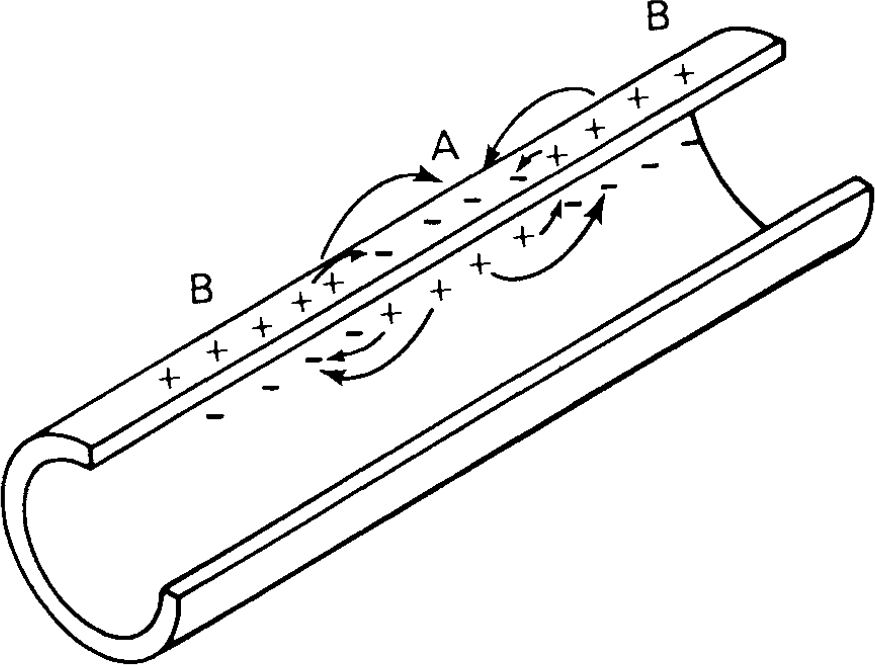
\includegraphics[height=5.2cm]{Background/depolarisation_wavefront}
	\caption[Spread of the depolarisation wavefront]{Spread of the depolarisation
	wavefront. When one region (A) of the neural membrane is depolarised, charge
	stored by the membrane capacitance is transferred from adjacent regions (B),
	thereby propagating depolarisation along the neuron. (Source:
	Reilly~\cite{reilly1998}. Copyright \textcopyright{} 1998, Springer.)}
	\label{fig:depolarisation_wavefront}
\end{figure}

In normal hearing listeners, depolarisation occurs due to the release of
neurotransmitters by stimulated hair cells~\cite{brown2001,martini2006} (recall
\S\ref{sect:normal_hearing}), so the wavefront only propagates in one direction:
away from the hair cell at the peripheral end. For \emph{electrically-evoked}
neural stimulation, the active electrodes set up an artificial electric
field, causing voltage disturbances along the membrane which drive ions across
the channels in the membrane~\cite{reilly1998}. The location of the stimulating
electrodes typically induces depolarisation somewhere in the middle of the
neuron, creating a bidirectional depolarisation wavefront
(Figure~\ref{fig:depolarisation_wavefront}).

Myelination of nerve fibres is a biological adaptation that permits faster
conduction velocities while retaining small fibre diameters~\cite{brown2001}.
Glial cells form a non-conductive \emph{myelin sheath} around the axon, with
small gaps between adjacent sheaths known as \emph{nodes of Ranvier}. The
structure means that ionic current can only cross the membrane at the nodes, so
the wavefront jumps along the axon from one node to the next instead of simply
to adjacent regions of the neural membrane. This process is known as
\emph{saltatory conduction}.

\subsubsection{Theoretical Models}

Several approaches are available for explaining the membrane behaviour. Early
models analysed current traversing a localised patch of neuronal membrane.
However, Reilly found that ``the force driving current into the membrane is the
external field distribution \emph{along the axon}, which cannot be described by
the current density at a single point''~\cite{reilly1998}. This suggests that
the spatial and temporal interactions along the entire length of the neuron must
be considered to properly represent action potential generation and
propagation~\cite{strelioff1973,rattay1990,reilly1998,astrom2014}. On the other
hand, a recent study of deep brain stimulation modelling found that activation
can be approximated without coupling the finite element solution to an axon
model~\cite{astrom2014}. Nonetheless, axon models are more likely to account for
spatial phenomena, such as the prevention of action potential propagation by a
sufficiently large ``anodal surround''~\cite{ranck1975}.

Many quantitative models of neural excitation have consequently been developed
based on cable theory, with the neuron being modelled as a long one-dimensional
cable as illustrated in Figure~\ref{fig:membrane_circuit}. McNeal's myelinated
nerve model~\cite{mcneal1976} was the first to consider stimulation due to
finite duration current pulses from extracellular electrodes. Here, the nodes of
Ranvier were spaced at regular intervals, and the myelin sheath was assumed to
be a perfect insulator. Only the central excitation node was modelled with
non-linear membrane conductances, so the model was applied to subthreshold
stimulation. Despite these simplifications, the McNeal model could account for a
variety of electrophysiological observations.

\begin{figure}
	\centering
	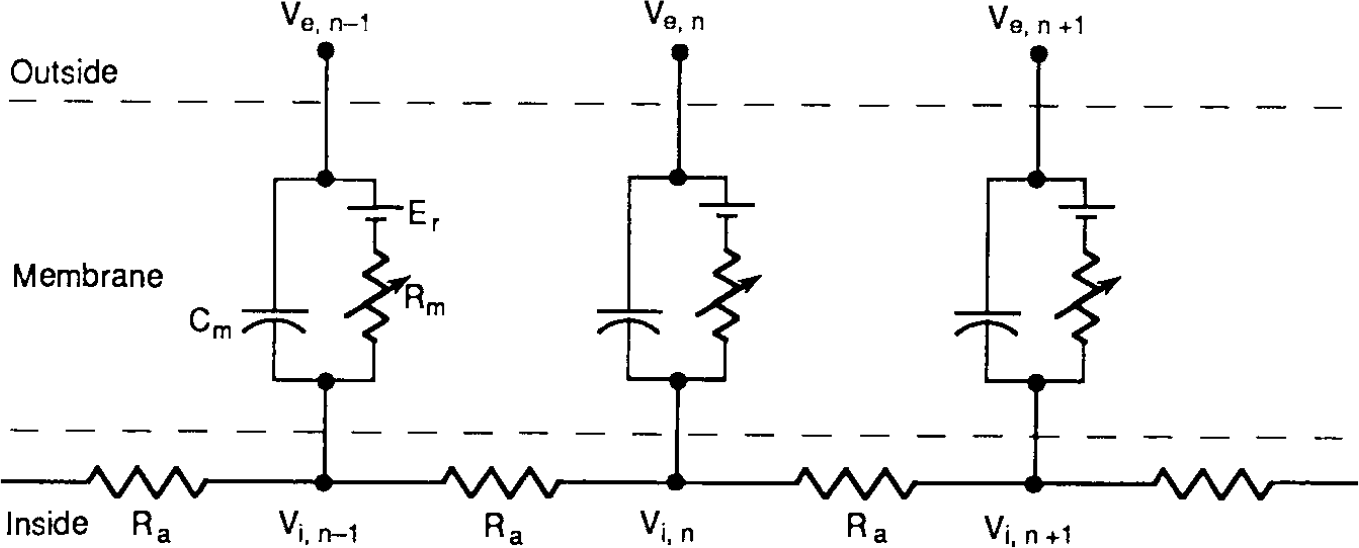
\includegraphics[height=5.1cm]{Background/mcneal_circuit}
	\caption[Equivalent circuit model for excitable membranes]{Equivalent circuit
	model for excitable membranes. (Source: Reilly~\cite{reilly1998}. Copyright
	\textcopyright{} 1998, Springer.)}
	\label{fig:membrane_circuit}
\end{figure}

Under this model, the membrane potential is described by:
\begin{equation}
	\frac{dV_n}{dt} = \frac{1}{C_m}[G_a(V_{n-1}-2V_n+V_{n+1}
	+V_{e,n-1}-2V_{e,n}+V_{e,n+1}) - I_{i,n}] \hspace{1em} (n \neq 0)
	\label{eqn:mcneal_membrane_potential}
\end{equation}
where $ V_n = V_{i,n} - V_{e,n} $ is the potential difference across the
membrane at the $ n $th node along the fibre (with a positive value indicating
depolarisation), $ t $ is time, $ C_m $ is the membrane capacitance of the node,
$ G_a = \nicefrac{1}{R_a} $ is the internodal conductance, $ V_{e,n} $ is the
external nodal voltage, and $ I_{i,n} $ is the internal ionic current flowing in
the node. The ionic current term can be modelled linearly using Ohm's law for
subthreshold stimulation, or non-linearly when at or near the excited state
using differential equations, such as those of Frankenhaeuser and
Huxley~\cite{frankenhaeuser1964}, or stochastic methods~\cite{bruce1999}.

In his review paper on empirical studies of electrical stimulation, Ranck found
that depolarisation was primarily caused by the extracellular voltage becoming
more negative (i.e. intracellular potential changes were
small)~\cite{ranck1975}. He also found that current flow along the long axis of
the neuron is more likely to depolarise it than transverse current. These
findings were strongly supported by McNeal's theoretical model. Subsequent
studies extended McNeal's basic framework. Reilly's spatially extended
non-linear node (SENN) model, for instance, implemented several non-linear
nodes~\cite{reilly1985} and gave further weight to the accepted tenet that
stimulation occurs where neurons end or bend, or where the spatial gradient of
the electric field is highest~\cite{reilly1998}. Colombo and Parkins modified
the McNeal neuron geometry to match measurements by Liberman and Oliver in the
cat~\cite{liberman1984}, and implemented additional non-linear
nodes~\cite{colombo1987}. Rattay made the framework more robust, accounting for
both subthreshold and superthreshold stimulation as well as both myelinated and
unmyelinated fibres~\cite{rattay1986}. He found that for electrical stimulation,
``the second derivative of the external potential in the direction of the axon
is responsible for all the activations inside the axon''~\cite{rattay1986}.
Since it was a necessary condition for neural excitation, Rattay called this the
\emph{activating function} (AF). The AF can be expressed for both unmyelinated
and myelinated neurons respectively as:
\begin{equation}
	\text{AF} = \frac{\partial {^2} V_e}{\partial x^2} \approx
	\frac{V_{e,n-1}-2V_{e,n}+V_{e,n+1}}{\Delta x^2}
	\label{eqn:af}
\end{equation}
where $ x $ is displacement along the nerve fibre. Further refinements to the
model were later added to make the model more applicable to human cochlear
neurons~\cite{rattay1999,rattay2001neuron}.

Another prominent excitation model in CI research is the generalised Schwarz,
Eikhof, and Frijns (GSEF) model developed by Frijns \etal~\cite{frijns1995},
intended for use in models of the guinea pig cochlea. This model was based on
earlier work by Schwarz and Eikhof with myelinated rat fibres~\cite{schwarz1987}
and Frijns and ten Kate's modifications of the SENN model~\cite{frijns1994}.
Like Colombo and Parkins, it was based on mammalian neural kinetics, with
non-uniform internodal lengths in accordance with the morphological data of
Liberman and Oliver~\cite{liberman1984}. Each nerve fibre included 16 non-linear
nodes. The assumption of perfectly insulating myelin sheaths was retained.

The main weakness in the majority of these models is that they mix empirical
results from different animal species. This does not necessarily invalidate the
model, since neural kinetics can be similar across species and the models are
tuned to fit experimental data, but there is still an abstraction gap between
these theoretical models and \insitu{} nerve fibres. This was particularly
evident in Whiten's modelling work~\cite{whiten2007} (see
\S\ref{sect:whiten})---despite having a patient-specific model with ideal
archival data for comparison, he found that the model was weakest when compared
against the psychophysical data. Other aspects of the modelling methodology may
have played a part in this discrepancy, suggesting that significant care and
attention to detail need to be exercised throughout the reconstruction process.

More recent developments in the area of neuronal modelling have been published
by a group in Melbourne, Australia. In a series of four
papers~\cite{meffin2012,tahayori2012,meffin2014,tahayori2014}, Meffin~\etal{}
developed a more robust model of extracellular stimulation that goes beyond the
cable theory models by incorporating the cellular composition of the neural
tissue, including the effect of the confined extracellular space, as well as
both longitudinal and transverse modes of stimulation. The formulation
calls for parallel unmyelinated neurons, which may be applicable to the
spiral ganglion, but has yet to be implemented in a VCM of the cochlea.

\section{Electric Models of the Cochlea}

Existing electric models of the cochlea fall into two categories: lumped-element
models and volume conduction models. Prominent examples are described in the
following sections, grouped by primary author and sorted in chronological order
of appearance.

% ========================================================================= LEMs

\subsection{Lumped-Element Models}
\label{sect:lumped_element_models}

\subsubsection{Von \bekesy{} (1951)}

Von \bekesy's LEM~\cite{vonbekesy1951} was the pioneering effort to understand
the electroanatomy of the cochlea. In his experimental work with explanted
guinea pig cochleae, von \bekesy{} found that the otic capsule was a good
insulator and mused that the grounding resistance must therefore lie in the
modiolus. Additional measurements indicated that ``the main grounding pathway of
the cochlea is through the acoustic nerve to the brain''~\cite{vonbekesy1951},
and that there would be substantial cross-conduction between the turns of the
cochlea because the nerves and blood vessels of the modiolus enter the cochlear
partition along the entire length of the spiral. These observations gave birth
to the idea that grounding the auditory nerve is a good choice for representing
the cochlea's electrical behaviour.

In light of these findings, von \bekesy{} sought to explain the attenuation
of voltage along the cochlear partition by considering two extreme cases:
(i)~the cochlear partition is a very \emph{poor} insulator, so the intracochlear
spaces would resemble a homogeneous conducting body (like a drop of fluid); and
(ii)~the cochlear partition is a very \emph{good} insulator, so the cochlea was
effectively a fluid-filled tube separated into two conjoined canals (analogous
to a \emph{transmission line}). He found that while neither extreme was
realistic for the entirety of the cochlea, the former was more suitable at the
helicotrema and the latter near the round window.

Focusing on the basal turn, he created the transmission line model in
Figure~\ref{fig:model_vonbekesy}. The model consisted of a 3D network of
resistive elements, representing current paths along the scala vestibuli, the
scala tympani, and the cochlear partition, the grounding pathway through the
nerves and blood vessels in the modiolus, and additional resistances to account
for cross-turn effects.

\begin{figure}
	\centering
	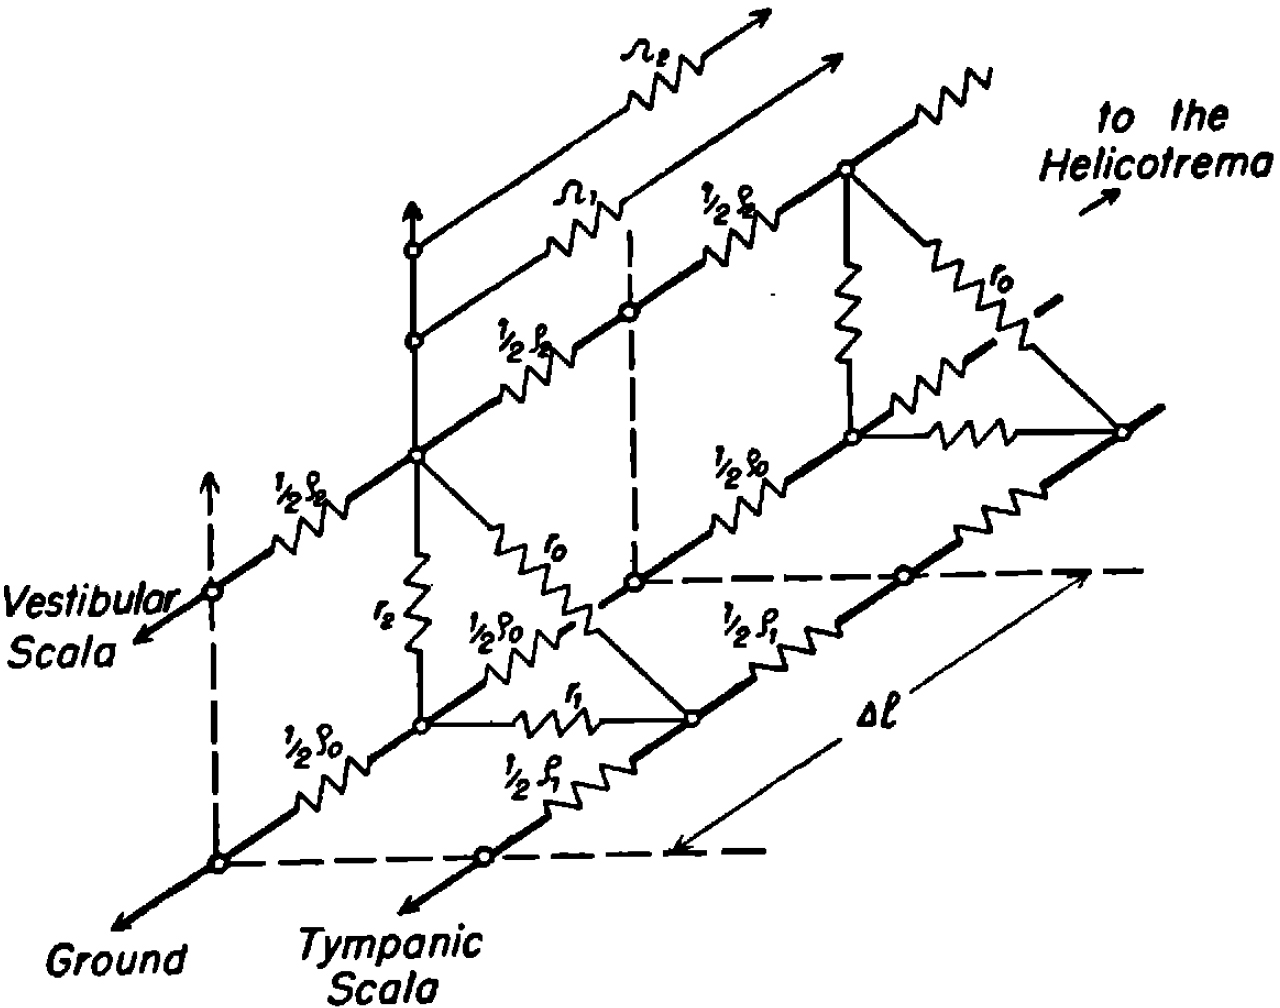
\includegraphics[height=6.8cm]{Background/vonbekesy_fig11a}
	\caption[The von \bekesy{} model]{The von \bekesy{} transmission line model,
	representing a small section of the cochlear tube near the basal end. (Source:
	von \bekesy~\cite{vonbekesy1951}. Copyright \textcopyright{} 1951,
	Acoustical Society of America.)}
	\label{fig:model_vonbekesy}
\end{figure}

The von \bekesy{} model was a good start to electroanatomical modelling of the
cochlea, but it had several shortcomings. The model accounted for many of the
possible current paths, but it failed to consider others like the scala media,
the cerebrospinal fluid (CSF), and the spiral ligament. Detail was also lost
where different tissue types were combined into single elements; for instance,
the organ of Corti and the basilar membrane were modelled together as the
cochlear partition, and the nervous and vascular pathways in the modiolus were
combined into a single grounding resistance. It is impossible to determine which
tissue path is preferred in these lumped regions. Von \bekesy{} also found that
capacitive effects were not important. However, the 1000 Hz stimulus signal used
in these impedance measurements is well below the 10 kHz threshold typically
required for such effects to manifest~\cite{geddes1967}.

\subsubsection{Johnstone \etal{} (1966)}

Johnstone~\etal{} were also interested in discovering more about the electrical
pathways of the guinea pig cochlea, particularly the resistances of the three
boundary walls of the scala media. They proposed a relatively simple LEM
(Figure~\ref{fig:model_johnstone}) that aimed to synthesise the measurements of
both von \bekesy{} and Misrahy~\cite{misrahy1958} into one consistent
model~\cite{johnstone1966}.

\begin{figure}
	\centering
	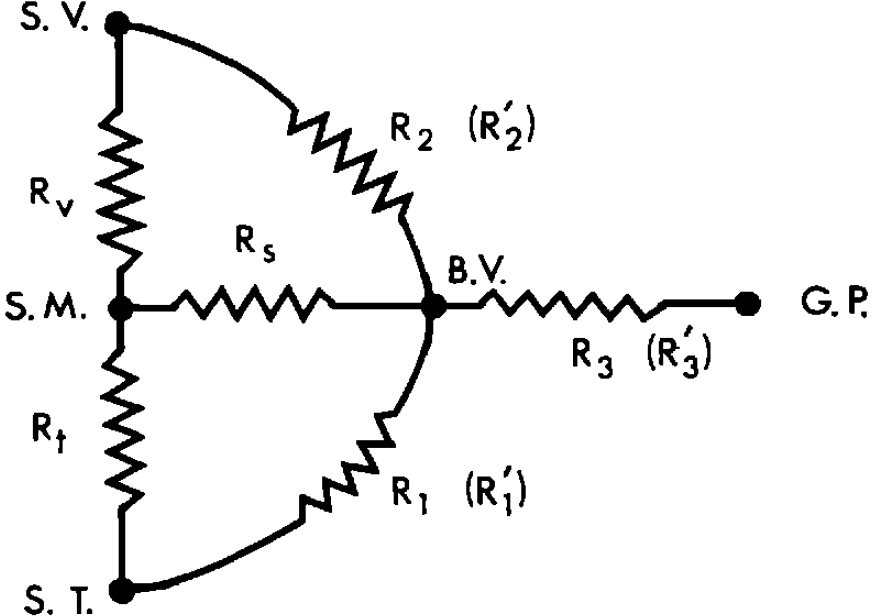
\includegraphics[height=4.8cm]{Background/johnstone}
	\caption[The Johnstone model]{The Johnstone model. SV=scala vestibuli; SM=scala
	media; ST=scala tympani; BV=blood vessels; GP=guinea pig (body). (Source:
	Johnstone~\etal~\cite{johnstone1966}. Copyright \textcopyright{} 1966,
	Acoustical Society of America.)}
	\label{fig:model_johnstone}
\end{figure}

The Johnstone model differs from the von \bekesy{} model in several respects. It
was devised as a 2D representation of the experimental setup through one turn of
the cochlea, and does not directly account for longitudinal current flow or
cross-turn effects. As per the focus of this study, the main pathways considered
were the boundaries of the scala media, i.e. Reissner's membrane, the organ of
Corti and associated structures on the basilar membrane, and the spiral ligament
via the stria vascularis. There is a strong emphasis on the role of the cochlear
blood vessels as a conductive pathway that links the scalae. Like von \bekesy,
Johnstone~\etal{} also suggested that the grounding resistance would be through
the structures of the internal auditory meatus, in conjunction with the cochlear
artery. The experimental technique used also differed, with the injection of
square current pulses akin to those used in contemporary CI systems, though with
a significantly longer pulse width.

Overall, the Johnstone model added some extra detail around the scala media
while ignoring detail from other regions of the cochlea. It still favoured a
purely resistive formulation. Johnstone~\etal{} admitted that the model was
``the simplest measurable network'', even
``oversimplified''~\cite{johnstone1966}, but was nonetheless able to reconcile
the results of earlier studies and provide reasonable voltage predictions.

\subsubsection{Strelioff (1973)}

Another LEM was proposed by Strelioff in 1973~\cite{strelioff1973} (see
Figure~\ref{fig:model_strelioff}). It aimed to study the spatial distribution of
electric potentials and currents in the guinea pig cochlea arising from acoustic
stimulation.

\begin{figure}
	\centering
	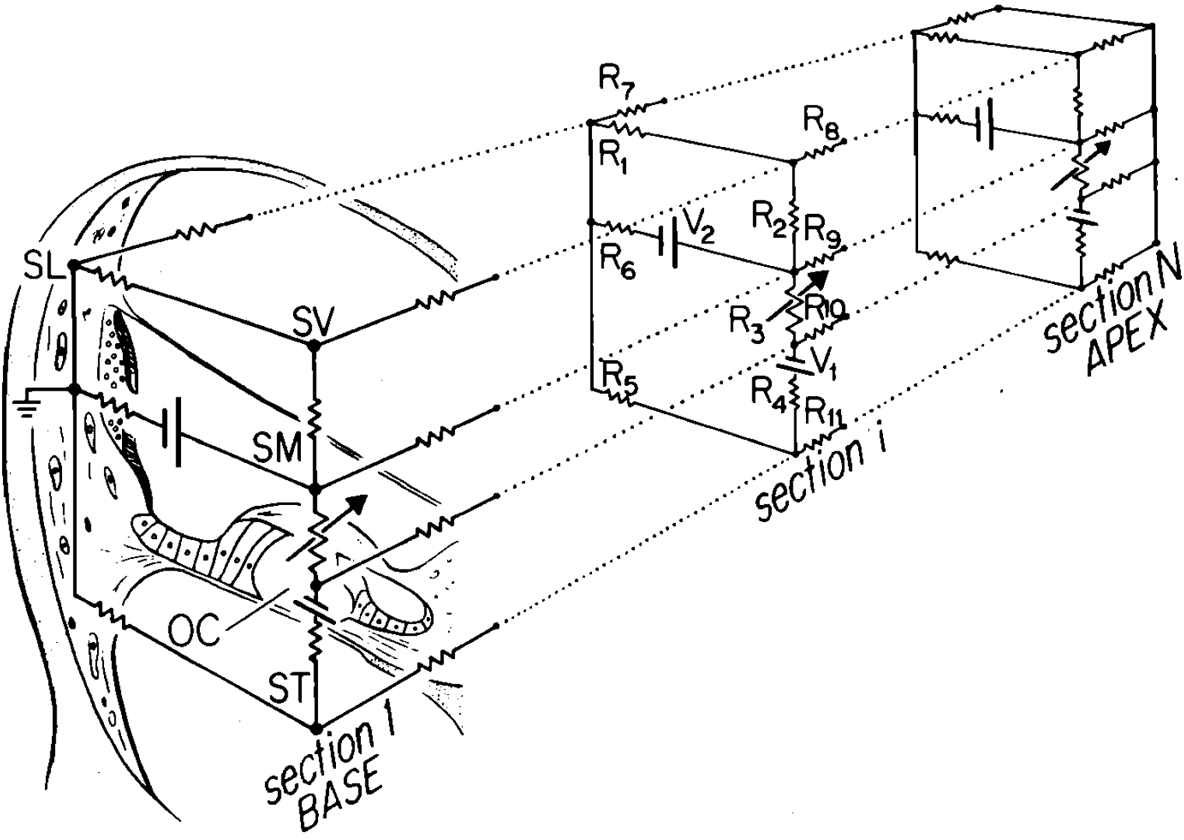
\includegraphics[height=6.5cm]{Background/strelioff}
	\caption[The Strelioff model]{The Strelioff model. SL=spiral ligament; SV=scala
	vestibuli; SM=scala media; OC=organ of Corti; ST=scala tympani. (Source:
	Strelioff~\cite{strelioff1973}. Copyright \textcopyright{} 1973,
	Acoustical Society of America.)}
	\label{fig:model_strelioff}
\end{figure}

In terms of the layout of the circuit elements, the Strelioff model was arguably
more accurate than either the von \bekesy{} or Johnstone models. It returned to
a linear 3D network similar to von \bekesy's model, with a series of over 90
cross-sectional circuits connected via longitudinal resistances. Each
cross-section included nodes in five different fluid-filled spaces (the scala
vestibuli, scala media, and scala tympani, the tunnel of Corti, and the spiral
ligament), resistances to represent the pathways between adjacent nodes, and
battery elements to represent endocochlear potentials.

Weaknesses of the Strelioff model include the decision to use a linear model to
represent the entire length of cochlear spiral, which ignores cross-turn effects
from the true 3D geometry. Lumping the longitudinal pathways along the modiolus
with those of the spiral ligament and ground is also questionable given that
they lie on opposite sides of the scalae. The cochlear vasculature is not
explicitly accounted for in the model, and no capacitive effects were
incorporated despite an admission that they undoubtedly exist. Strelioff also
noted that the use of discrete elements could reduce accuracy, but estimated
that the results were accurate to within 5\% of a continous model based on an
extrapolation of some preliminary results.

\subsubsection{Black and Clark (1980)}

The Black and Clark model~\cite{black1980,black1983}, shown in
Figure~\ref{fig:model_black}, was the first effort to investigate the behaviour
of the cochlea during electrical stimulation for hearing restoration. The
geometry of the model was based on that of Johnstone \etal, but extended to 16
cross-sections in the transverse direction as per the transmission line models.
Resistance values were fitted to the range of published experimental
measurements via scaling.

\begin{figure}
	\centering
	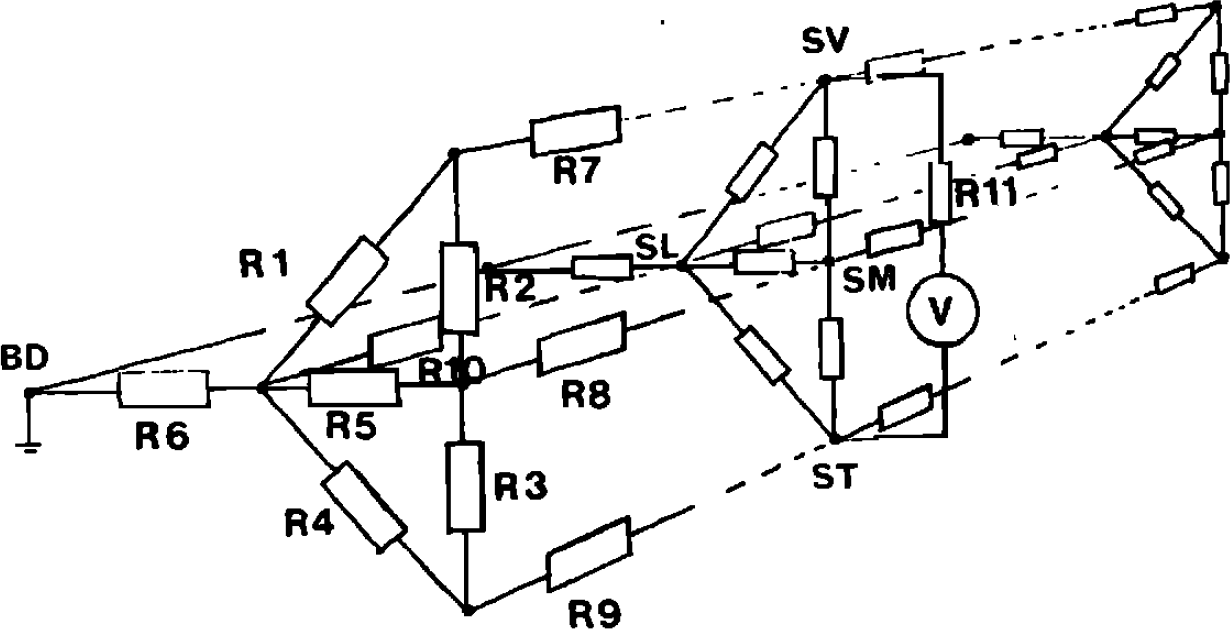
\includegraphics[width=9cm]{Background/black_clark}
	\caption[The Black and Clark model]{The Black and Clark model. SV=scala
	vestibuli; SM=scala media; ST=scala tympani; SL=spiral ligament; BD=animal
	body. (Source: Black and Clark~\cite{black1980}. Copyright \textcopyright{}
	1980, Acoustical Society of America.)}
	\label{fig:model_black}
\end{figure}

In conjunction with some additional measurements, the model revealed differences
in stimulation specificity between various electrode configurations; in
particular, that BP stimulation resulted in the highest specificity of the
tested configurations. They also noted that the spread of current through the
neural tissues may be different from the spread of potentials through the
scalae, so voltage traces on their own were insufficient for inferring the
effect on neural excitation.

Since they use the same circuit layout for the cross-sectional slices, this
model shares some of the weaknesses of the Johnstone model. An additional
concern of this study lies in the continual rescaling of model parameters to
force-fit the experimental data. The authors acknowledged in the discussion that
the model was too simple for some applications, such as modelling length
constants under BP stimulation.

\subsubsection{Suesserman and Spelman (1993) \& Machado and Toumazou (1995)}

In their studies of the cochlea, Suesserman and Spelman realised that the
physical presence of the electrode array and the deterioration of cochlear
structures with the onset of deafness both had an effect on the current paths,
which had not been accounted for in the modelling literature. As such, they
created an extension of the Strelioff model to better match the \invivo{}
electrical behaviour during electrical stimulation~\cite{suesserman1993}.

Their model represented the first turn of the cochlea using 51 cross-sectional
slices with a thickness of 200 $ \upmu $m, as illustrated in
Figure~\ref{fig:model_suesserman}. It added a new node for the stimulating
electrode in the scala tympani and new elements to capture the membrane
capacitances ignored in previous studies. The battery elements representing
endocochlear potentials were removed since the focus was on exogenous
stimulation. The model parameters were adjusted to account for the increase in
resistance along the scala due to the presence of the electrode array and
matched to Spelman's earlier experimental work on implanted guinea pig
cochleae~\cite{spelman1982}.

\begin{figure}
	\centering
	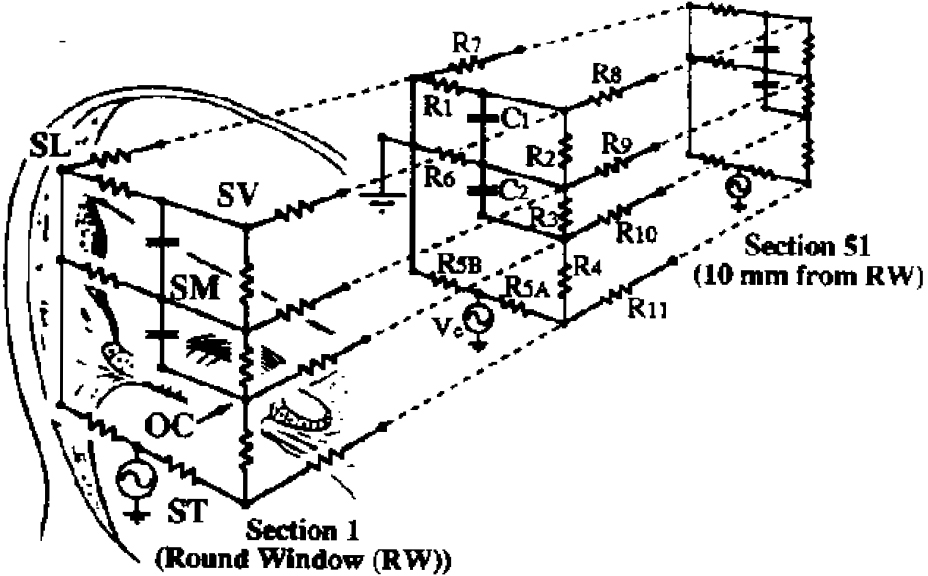
\includegraphics[height=6cm]{Background/suesserman}
	\caption[The Suesserman and Spelman model]{The Suesserman and Spelman
	model. SL=spiral ligament; SV=scala vestibuli; SM=scala media; OC=organ of
	Corti; ST=scala tympani. (Source: Suesserman and
	Spelman~\cite{suesserman1993}. Copyright \textcopyright{} 1993, IEEE.)}
	\label{fig:model_suesserman}
\end{figure}

The Suesserman and Spelman model was the most accurate LEM of the implanted
cochlea. However, like prior studies, it assumed that the cochlea could be
uncoiled. With the emphasis firmly on the modelling of electrical stimulation,
it is important to consider that the neural structures closer to the modiolus
were still not included since the uncoiling assumption becomes less applicable
in this central region of the cochlea. The authors noted that induced fields
from CI stimulation would distort each other due to coupling between adjacent
turns of the cochlea, but justified the exclusion of these effects in the model
by saying that these distortions are quite small~\cite{girzon1987} and that
psychophysical experiments had indicated minimal impact on overall sound
perception~\cite{townshend1987}.

In 1995, Machado and Toumazou further extended the model by deriving
approximating equations for each of the model parameters~\cite{machado1995}.
These allowed the model to be used for all turns of the guinea pig cochlea, and
for other species to be studied qualitatively as well.
The model was heavily reliant on the earlier assumption that cross-turn effects
were negligible. Machado and Toumazou went on to use their refined model to
propose additional design considerations for CI system
architectures~\cite{machado1996}.

Jolly also used the Suesserman and Spelman model to evaluate the feasibility of
quadrupolar stimulation~\cite{jolly1996}.

\subsubsection{Kral \etal{} (1998)}

A comprehensive study comparing the spatial resolution of various electrode
configurations was undertaken by Kral \etal{} in 1998. It featured \invitro,
\invivo{} (cadaveric and live cats), and \insilico{} components.

The LEM featured in this study is shown in Figure~\ref{fig:model_kral}. Kral
\etal{} modelled the implanted scala tympani by using an axisymmetric assumption
on the unrolled cochlear geometry, accounting for the change in cross-sectional
area along the chamber. Material properties were sourced from prior experimental
work and models, and neural excitation was modelled using a current trigger
level on the elements representing the peripheral processes or the spiral
ganglion. The selected threshold currents produced a good fit with the \invivo{}
neuronal data. The study results showed that TP stimulation elicited the
sharpest spatial tuning curves, implying focused stimulation, and that the
current paths followed by injected current are important in determining spatial
selectivity.

\begin{figure}
	\centering
	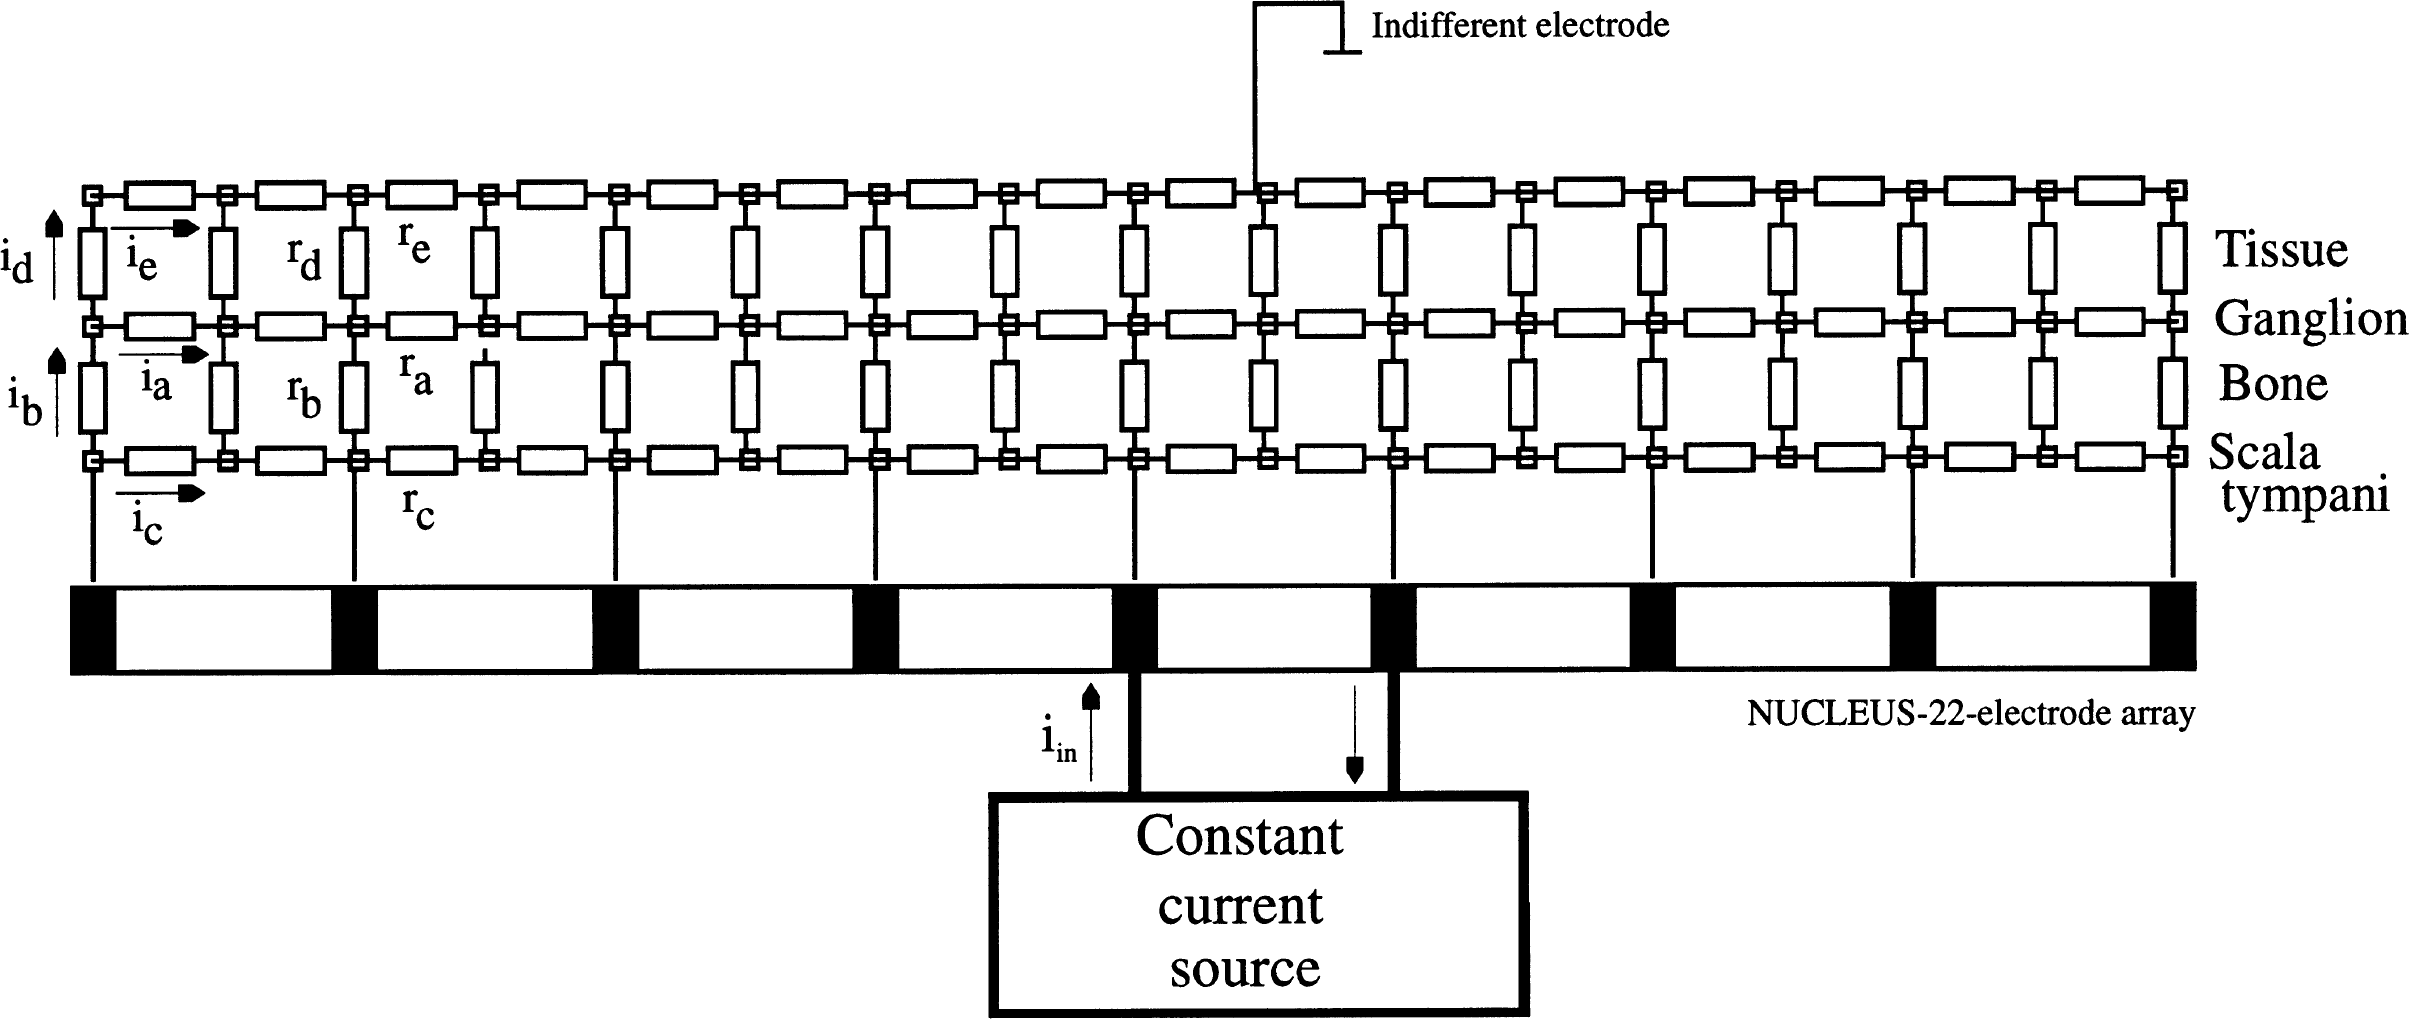
\includegraphics[width=\textwidth]{Background/kral}
	\caption[The Kral model]{The Kral model. (Source: Kral~\cite{kral1998}.
	Copyright \textcopyright{} 1998, Elsevier B.V.)}
	\label{fig:model_kral}
\end{figure}

The primary limitation of the model is that it used a simplified 2D geometry, so
excitable structures near the modiolar wall of the scala tympani were considered
but the nerve tissue in the modiolus was poorly represented. The influence of
other nearby fluid chambers (the scalae media and vestibuli) are not considered,
even though the scala tympani is not perfectly insulated. In addition, it was
comprised of resistive elements only and so did not consider time- and
frequency-dependent effects, which are observed in \invivo{} measurements.

\subsubsection{Vanpoucke \etal{} (2004)}

Vanpoucke \etal{} created an LEM of the cochlea to help interpret data from an
electrical field imaging (EFI) study~\cite{vanpoucke2004identification}. EFI
data were sourced because it is a simple, non-invasive, and rapid measurement
technique. The complete model, shown in Figure~\ref{fig:model_vanpoucke}, is
roughly equivalent to the Kral model in the sense that the network was
structured according to the layers of materials encountered by injected current.
The circuit itself was, however, quite different. It built upon a purely
resistive tissue model introduced in an earlier paper~\cite{vanpoucke2004facial}
and, like the Johnstone model, includes an element representing the total
resistance between the cochlea and the MP reference electrode. Additional
elements were introduced to represent the interface impedance for each
intracochlear electrode contact. All model parameters were then calculated from
experimental measurements using numerical methods.

\begin{figure}
	\centering
	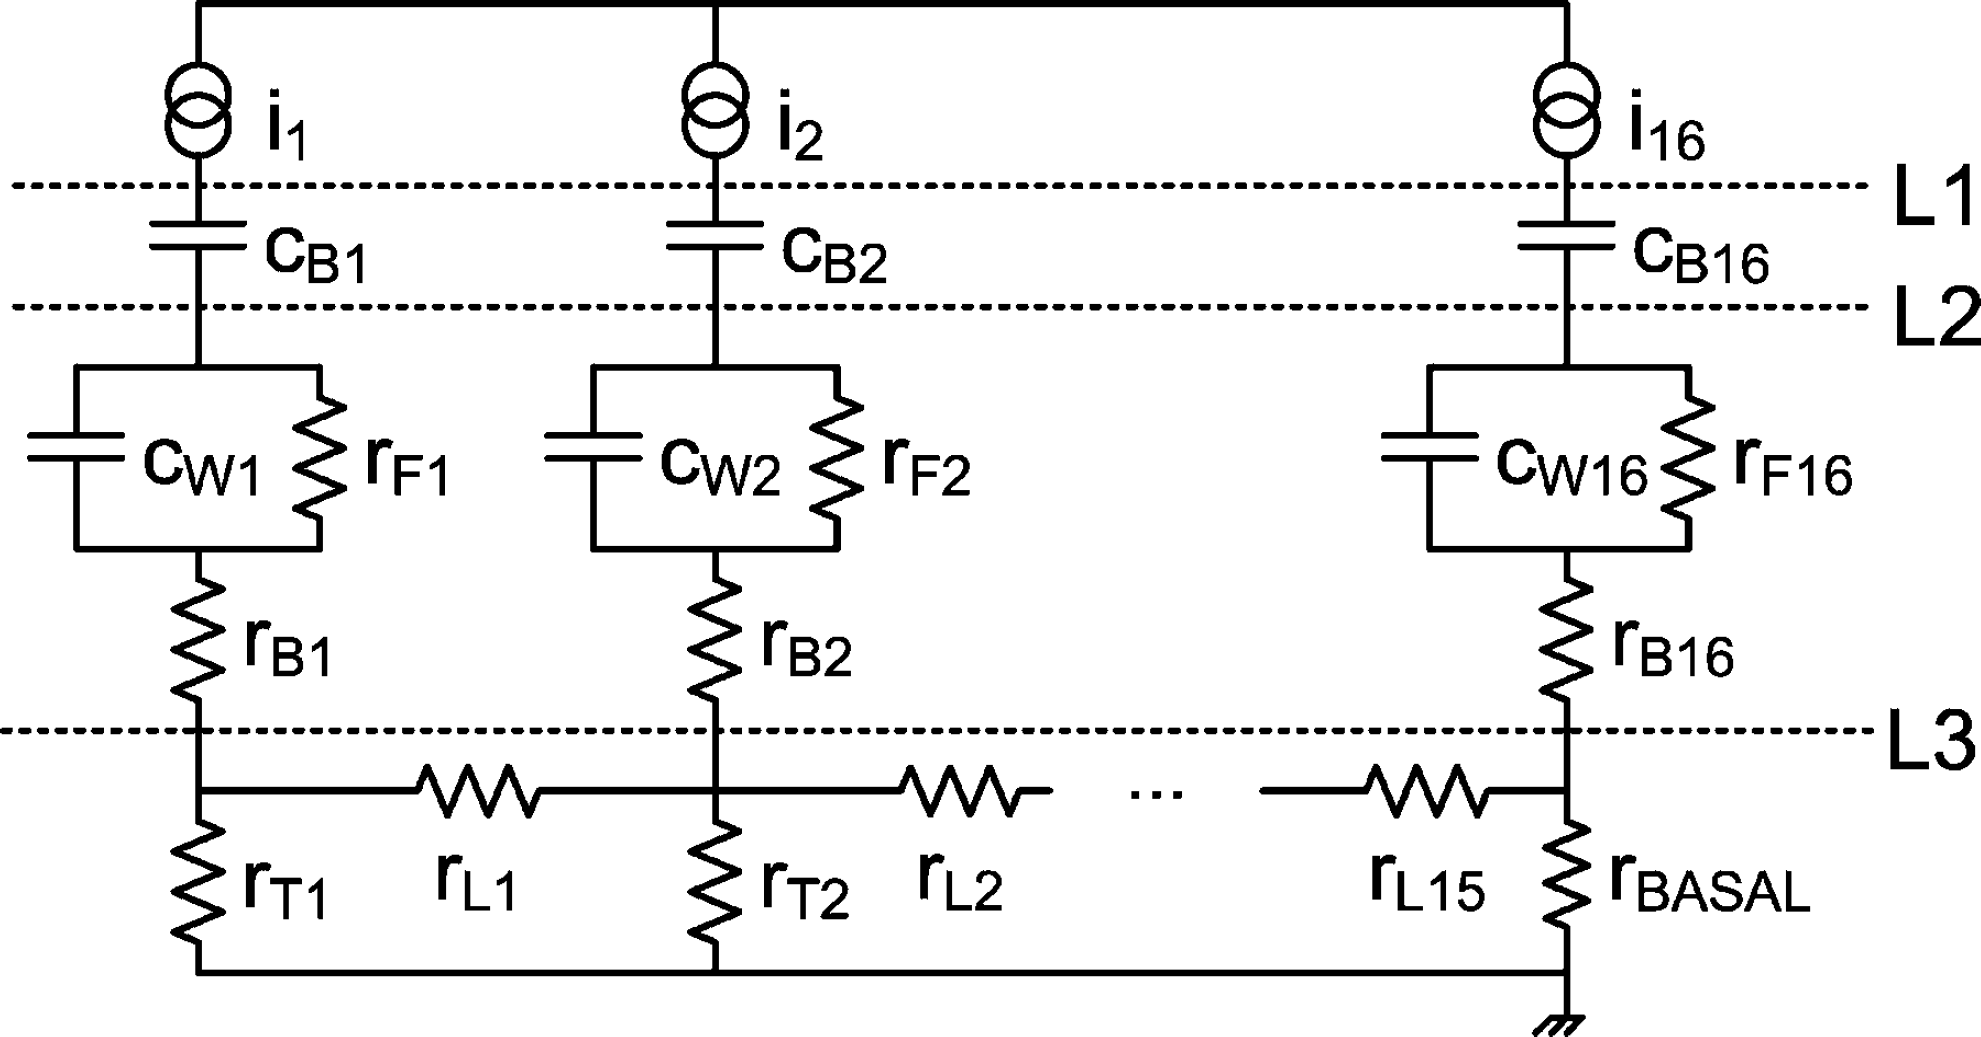
\includegraphics[width=9cm]{Background/vanpoucke}
	\caption[The Vanpoucke model]{The Vanpoucke model. (Source:
	Vanpoucke~\cite{vanpoucke2004identification}. Copyright \textcopyright{} 2004,
	IEEE.)}
	\label{fig:model_vanpoucke}
\end{figure}

The model provided a good match to the EFI data and was able to provide some
insight into the local conductive pathways near the stimulating electrode. There
was some concern about the interpretation of some unanticipated results.
Simplifications made in the construction of the circuit model, such as the use
of a linear tube geometry and the exclusion of the other scalar pathways, are
likely weaknesses in this representation.

% ========================================================================= VCMs

\subsection{Volume Conduction Models}
\label{sect:volume_conduction_models}

% 1987
\subsubsection{Girzon (1987)}

Girzon was one of the first to recognise that representing gross structures as
single nodes or elements was inadequate. He argued that in LEMs, the true 3D
structure of the inner ear is simplified, so some current paths are ignored. The
use of bulk impedance measurements between two points only reveals the
\emph{effective} impedance between them, and does not clearly demonstrate the
spatial pathway traversed by injected current. In addition, the representation
of implanted electrodes as point sources could be inaccurate since the arrays
occupy a substantial volume within the scala and have significantly different
electrical properties relative to the surrounding fluids.

In order to overcome these problems a new type of model was required, leading
Girzon to develop the first VCM of the cochlea (illustrated in
Figure~\ref{fig:model_girzon})~\cite{girzon1987}. By preserving the 3D,
heterogeneous structure of the cochlea, it was hoped that the VCM would be
``electro-anatomically accurate'' and could uncover insights that could not be
revealed using LEMs, such as the true current pathway to ground and the
resultant patterns of neural excitation.

\begin{figure}
	\centering
    \begin{subfigure}[t]{0.4\textwidth}
        \centering
        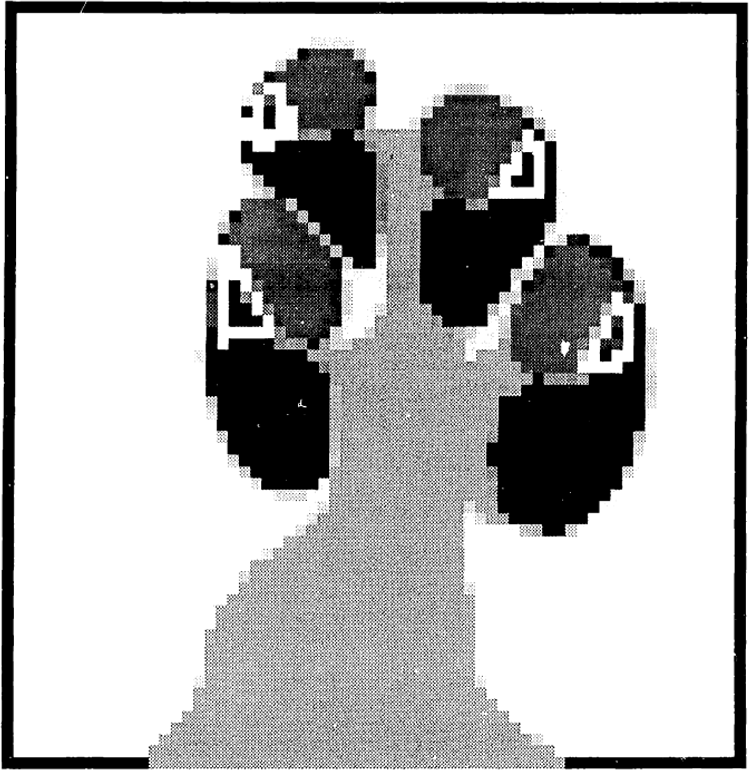
\includegraphics[height=6cm]{Background/girzon_section}
        \caption{ }
        \label{fig:girzon_section}
    \end{subfigure}
    ~~~~
    \begin{subfigure}[t]{0.52\textwidth}
        \centering
        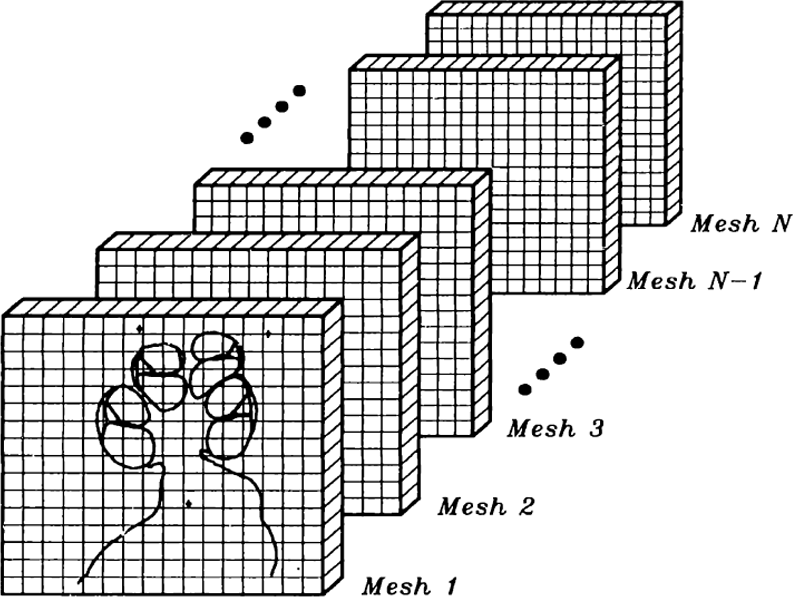
\includegraphics[height=6cm]{Background/girzon_slices}
        \caption{ }
        \label{fig:girzon_slices}
    \end{subfigure}
    \caption[The Girzon model]{The Girzon model. (a) A downsampled mid-modiolar
	section was mapped onto a finite difference grid. (b) The entire model
	consisted of $ N=40 $ slices. (Source: Girzon~\cite{girzon1987}. Copyright
	\textcopyright{} 1987, MIT.)}
	\label{fig:model_girzon}
\end{figure}

The model comprised of a volumetric geometry based on a set of serial sections
of a whole human cochlea. The overall size of the domain was 9.6$ \times $5.76$
\times $7.4 mm. Each section was hand-traced, vectorised, and downsampled to a
128$ \times $128$ \times $40 finite difference mesh
(Figure~\ref{fig:girzon_slices}). Tissue-specific resistivity values were used
as opposed to bulk resistance measurements between arbitrary points. These were
estimated from a variety of sources. Electrical loads were modelled as point
sources within the scala tympani. In terms of boundary conditions, the model was
insulated on all sides (as shown by the black outline in
Figure~\ref{fig:girzon_section}), except for the bottom surface where the
cochlear nerve exited the volume, which was grounded due to its ``electrical
proximity'' to the MP return electrode.

Girzon's VCM was a solid first attempt at creating a true 3D representation of
the electrically stimulated cochlea. He recognised that the key advantage of
this model over LEMs was that it allowed results to be interpreted in a more
accurate spatial context---for instance, the magnitude and direction of field
quantities could be calculated throughout the structure, and indirect current
pathways linking the turns of the cochlea were demonstrated. The model was
successfully used to investigate the effects of several parameters, including
the distribution of electric potential in the scala tympani, the accuracy of
modelling electrodes as point sources, the impact of model resolution, the
effects of material models and properties, and various modes of stimulation.
Validation against \invivo{} experimental measurements showed that the VCM was
superior to transmission line formulations.

Girzon acknowledged that as a first attempt, the model was subject to a number
of drawbacks. Regarding methodology, he suggested that the FEM would have been a
better solution method since it allows for non-uniform element dimensions, but
the FDM was more practical given the compromises between software and hardware
capabilities at the time.

In terms of tissue modelling, the resolution was quite low due to the
constraints in imaging technology. This meant that fine structures such as the
cochlear vasculature could not be reconstructed despite being a highly
conductive pathway. Girzon reasoned that the larger volume of the auditory nerve
made it a more significant path to ground, so the effect of vasculature was
likely to be small. Nonetheless, he called for further investigation of the
blood vessel pathways. The electrical conductivities of several
cochlear-specific tissues were probably also inaccurate since they had not been
measured and were instead based on conductivities of similar tissues that had
been published in the literature. Capacitive effects were ignored on the basis
that the perilymph, nerve, and blood vessels, which were likely to be the
dominant current carrying pathways, had been shown to be primarily resistive at
frequencies of up to 10~kHz~\cite{schwan1957capacitive,geddes1967,spelman1982}.

Finally, Girzon acknowledged that modelling the electrodes as simple point
sources was likely to have overestimated the current densities. He compared the
point source with a small near-spherical volume source and did not find a large
discrepancy in the voltage profile, but only after scaling to the maximum
potential in each trace. The staircase effect would have added to the modelling
error because the spherical current source could not be aligned to the Cartesian
grid. In addition, although grounding the nerve may seem reasonable for LEMs,
prescribing it in a VCM is incorrect since the spatial effects of this boundary
condition are not properly considered. Girzon simply reasoned that it would be
better than grounding all the model boundaries because the potential should be
asymmetric and he did not want to overestimate the voltage attenuation.

% 1990
\subsubsection{Finley \etal~(1987--1990)}

Finley \etal{} improved upon the work of Girzon in a few key areas. Their models
of the human cochlea were based on the FEM, and included volumetric
representations of the implanted electrode array. They started with a simple
two-dimensional (2D) model~\cite{finley1987}, but later extended it into a more
substantial 3D model~\cite{finley1989,finley1990}, shown in
Figure~\ref{fig:model_finley}. These VCMs were used to predict the induced
electric fields within the cochlea tissues, similar to Girzon's work. However,
they also went a step further and coupled it with a neural model to predict the
response of auditory nerve fibres, thereby providing a more complete view of the
CI stimulation process.

\begin{figure}
	\centering
	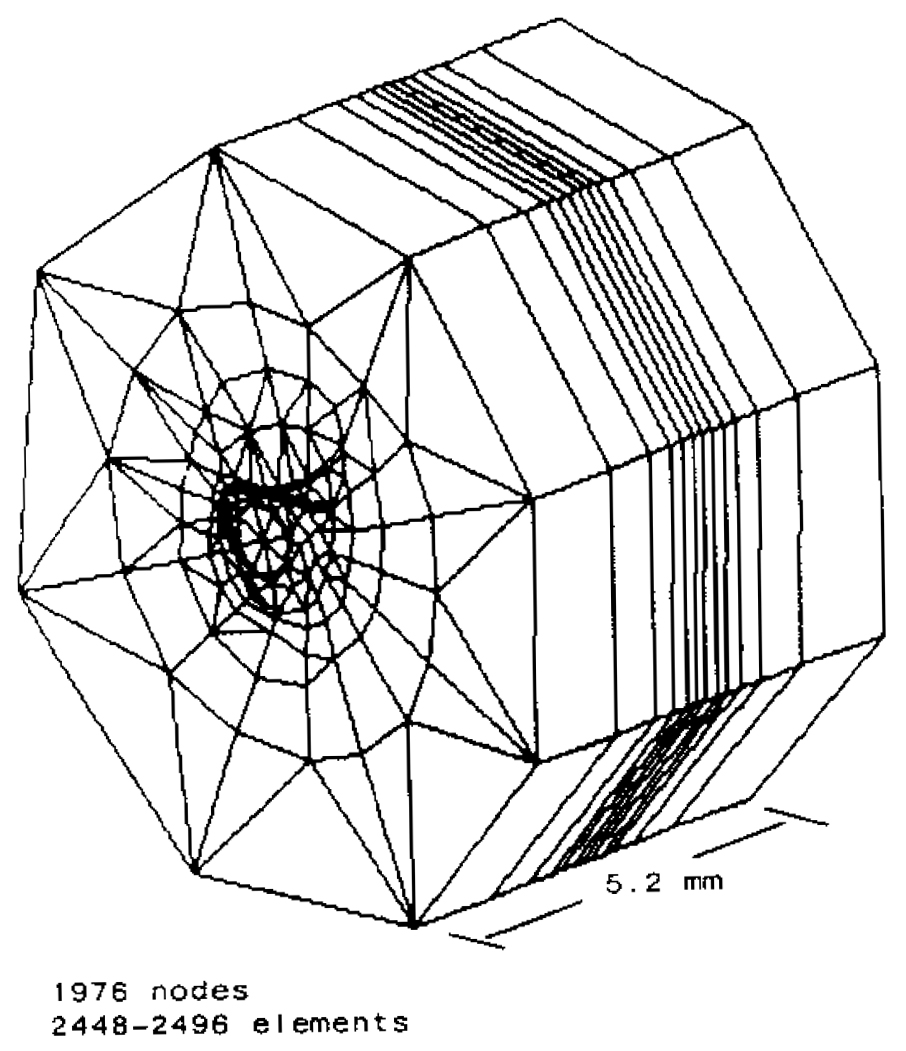
\includegraphics[height=8cm]{Background/finley}
	\caption[The Finley model]{The Finley model. (Source: Finley
	\etal\cite{finley1990}. Copyright \textcopyright{} 1990, Springer.)}
	\label{fig:model_finley}
\end{figure}

The geometry of the Finley model is best described as being extruded. A
histological image of one turn of the cochlea was segmented into various tissues
and discretised, with a higher mesh density in the central regions of the
cochlea. This 2D mesh was extended using prismatic elements to form a slab, and
twelve such slabs were then put together to generate a short, straight section
of the cochlear tube totalling 5.2 mm in length, resembling a short transmission
line model. The slabs closer to the mid-plane of the model were thinner, so the
mesh density was significantly higher in the central regions of the model than
at the periphery. Purely resistive tissue properties were assigned, and a
variety of bipolar electrode configurations were tested. Rattay's activating
function~\cite{rattay1986,rattay1990} was used to predict the likelihood of
excitation along seven neural trajectories.

Finley \etal~found that the model was quite useful for studying various bipolar
electrode configurations. The electrical fields and neural responses were highly
dependent on the arrangement of the source and sink electrodes, as well as the
location of the implanted array within the scala tympani. The greater anatomical
detail and improved (albeit still crude) electrode geometry, made possible
through the use of the FEM and by focusing on only one turn of the cochlea,
helped to increase the accuracy of the predicted electric field distribution
relative to other models.

Nonetheless, omitting the curvature of the cochlea was a step backwards from the
true 3D shape of the Girzon model. The authors indicated that greater anatomical
detail would have been preferred, such as in the lateral wall (i.e.~the spiral
ligament and stria vascularis) and in the modiolus. Unlike the Girzon study
though, the influence of blood vessels was not mentioned at all. The model's
limited spatial domain meant that broadly spreading monopolar fields could not
be considered. It also retained the use of purely resistive material models,
citing Spelman's experimental results~\cite{spelman1982}.

% 1995 (to present)
\subsubsection{Frijns \etal{} (1995--2015)}

The Frijns group is the most active in the field of cochlear modelling. They
have been iterating on their model since 1995, leading to what is rightfully
considered to be the most anatomically realistic representation (see
Figure~\ref{fig:model_frijns_evolution}). The Frijns model is therefore
considered to be the gold standard in this field. As per Finley \etal, it
consists of two coupled sub-models: an electrical VCM, this time based on the
BEM, and a neural excitation model (the generalised SEF model by
Frijns~\cite{frijns1995}), which uses the calculated potential
distribution to predict the electrically-evoked neural response.

\begin{figure}
	\centering
    
    \begin{subfigure}[t]{0.45\textwidth}
        \centering
        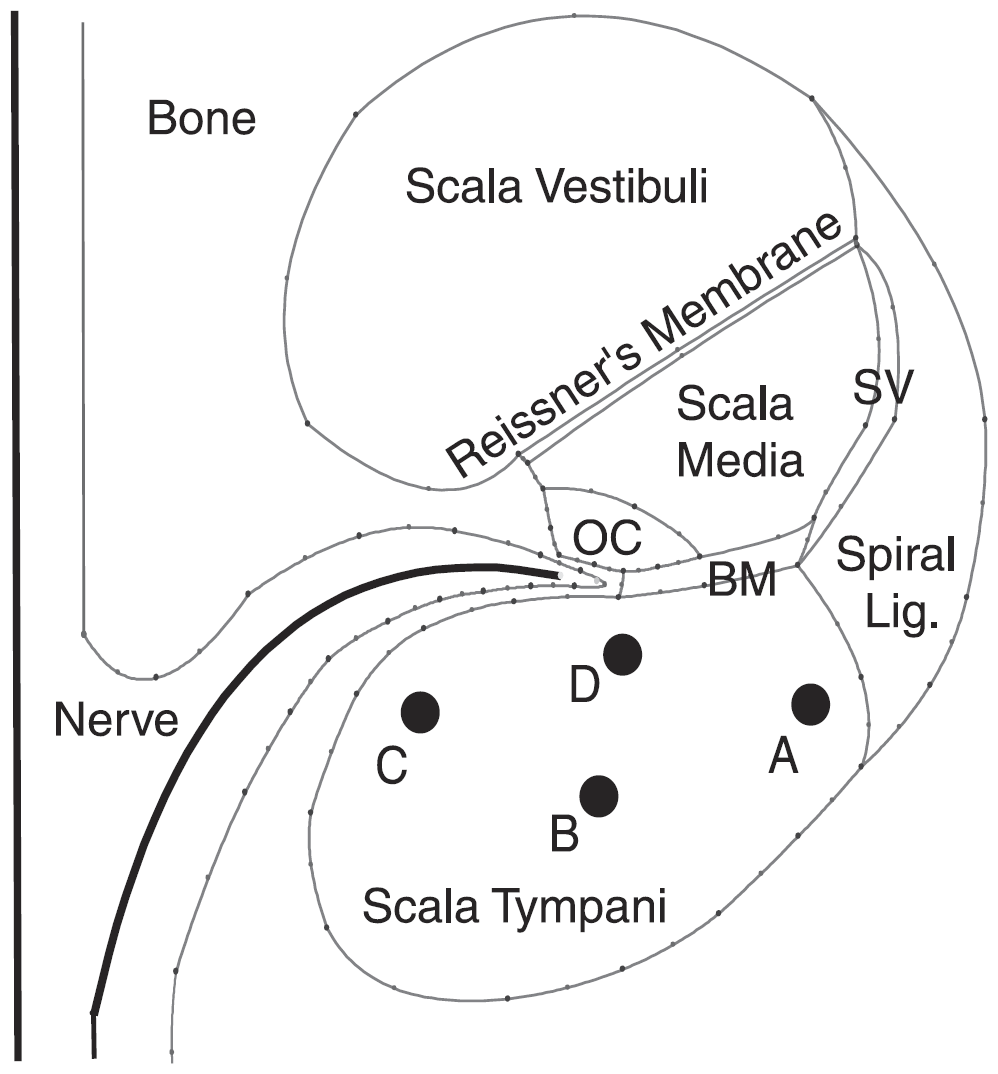
\includegraphics[height=5.1cm]{Background/frijns_spiral_schematic}
        \caption{ }
        \label{fig:frijns_tissues}
    \end{subfigure}%
    ~~~~
    \begin{subfigure}[t]{0.45\textwidth}
        \centering
        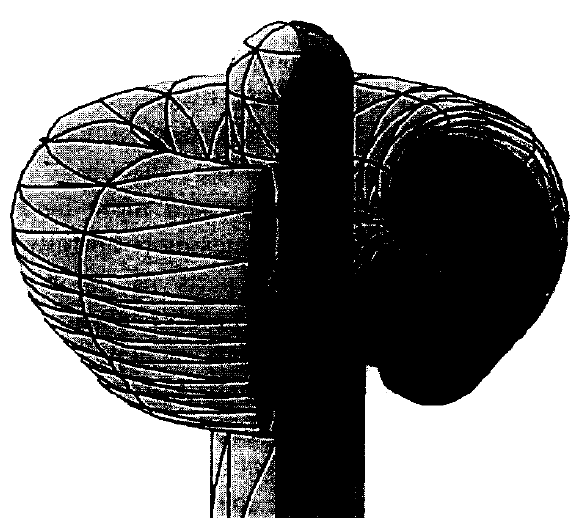
\includegraphics[height=5.1cm]{Background/frijns_rot_mesh}
        \caption{ }
        \label{fig:frijns_rot-1}
    \end{subfigure}%
	\vspace{0.5cm}
	
	\begin{subfigure}[t]{0.45\textwidth}
        \centering
        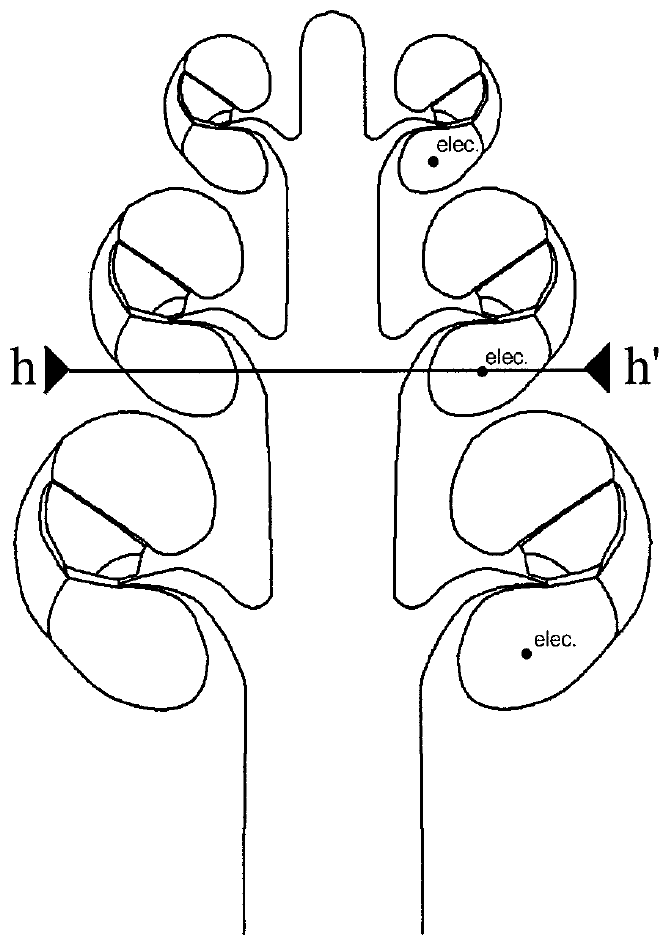
\includegraphics[height=6cm]{Background/frijns_rot-2_schematic}
        \caption{ }
        \label{fig:frijns_rot-2}
    \end{subfigure}%
    ~~~~
    \begin{subfigure}[t]{0.45\textwidth}
        \centering
        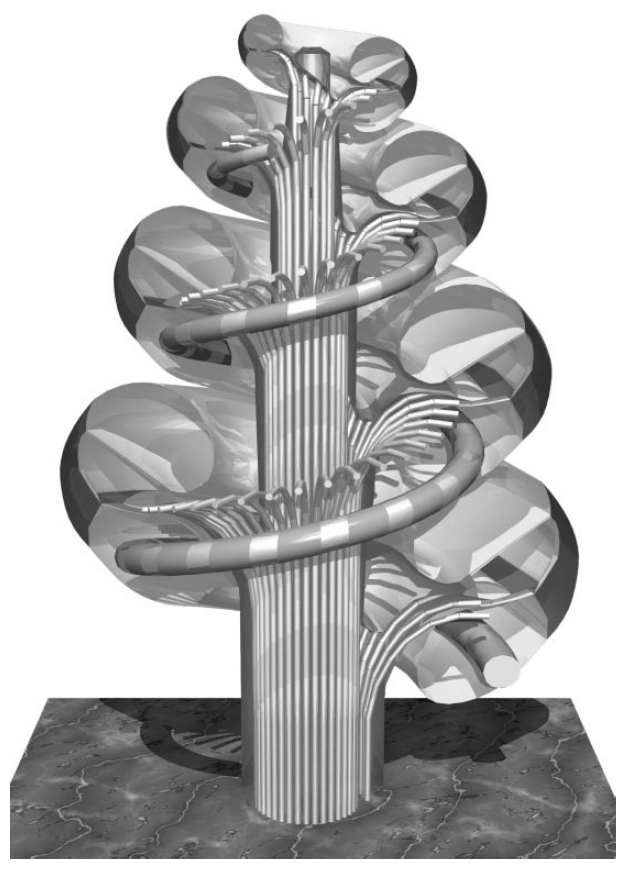
\includegraphics[height=6cm]{Background/frijns_spiral_surf}
        \caption{ }
        \label{fig:frijns_spiral}
    \end{subfigure}%
	\vspace{0.5cm}
    
    \begin{subfigure}[t]{0.45\textwidth}
        \centering
        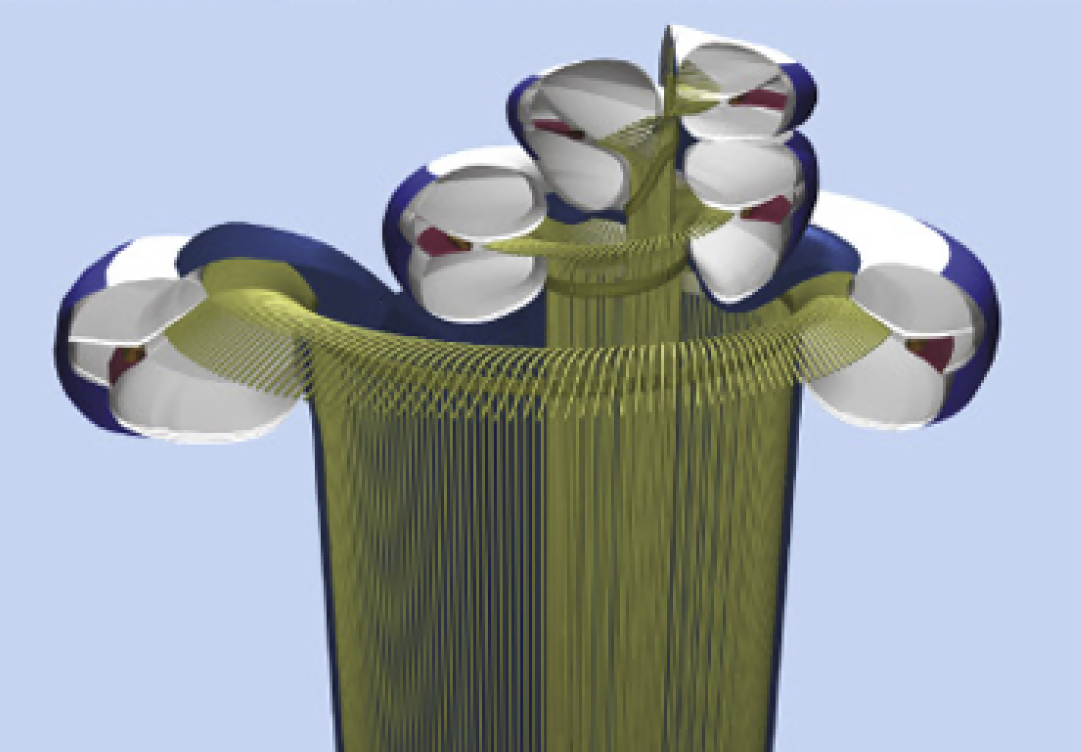
\includegraphics[height=4.75cm]{Background/frijns_human-1_surf}
        \caption{ }
        \label{fig:frijns_human-1}
    \end{subfigure}%
    ~~~~
    \begin{subfigure}[t]{0.45\textwidth}
        \centering
        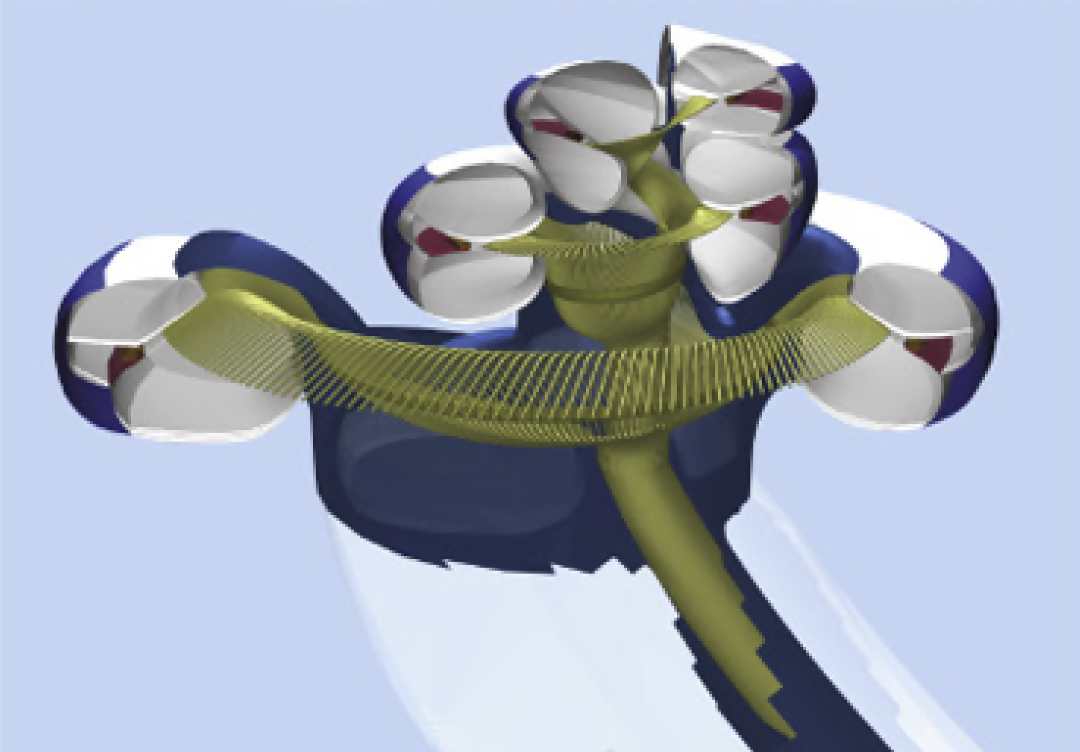
\includegraphics[height=4.75cm]{Background/frijns_human-2_surf}
        \caption{ }
        \label{fig:frijns_human-2}
    \end{subfigure}%
    
    \caption[Evolution of the Frijns model]{Evolution of the Frijns model over
    time. (a) Cross-sectional schematic showing the modelled cochlear
    tissues~\cite{frijns2000}; (b) the original axisymmetric
    model~\cite{frijns1995}; (c) the extended axisymmetric
    model~\cite{briaire2000field}; (d) the spiral model~\cite{frijns2000}; (e)
    the original human model~\cite{frijns2001,kalkman2014}; (f) the refined
    human model~\cite{kalkman2014}. (Copyright \textcopyright{} 1995--2014,
    Elsevier B.V.; 2001, Wolters Kluwer.)}
	\label{fig:model_frijns_evolution}
\end{figure}

The initial model~\cite{frijns1995,frijns1996} was based on a histological
section from a guinea pig cochlea~\cite{frijns1995}. An image of the second turn
was digitised, segmented and revolved to form a ``rotationally symmetric'' (i.e.
axisymmetric) toroidal structure (see Figures~\ref{fig:frijns_tissues} and
\ref{fig:frijns_rot-1}). The segmented tissues were embedded in a surrounding
domain of bone. Due to the use of the BEM, the thicknesses of the cochlear
membranes had to be increased to avoid excessive numerical errors, so their
conductivities were magnified proportionally. Conductivity values for the other
tissues were either sourced directly from existing literature or calculated from
published resistance and morphological data. Electrodes were modelled as point
sources located in one of four positions, marked as points A through D in
Figure~\ref{fig:frijns_tissues}. Only BP stimulation was modelled.

Frijns~\etal{} went on to compare this model with existing efforts. They showed
that relative to straight models, such as those of Finley \etal\cite{finley1990}
and Suesserman and Spelman~\cite{suesserman1993}, the calculated potential
fields are significantly different~\cite{frijns1995}, so the assumption of an
unrolled cochlear geometry was invalid. They also showed that Finley~\etal's
omission of the spiral ligament, stria vascularis, and organ of Corti resulted
in an inaccurate representation of the scala media. These three tissue
boundaries act as an insulating layer and help to maintain the endocochlear
potential. Further refinements to the model, including more fine detail,
anisotropic conductivities, and realistic electrode shapes were also discussed.

The guinea pig model was further developed in some later
papers~\cite{briaire2000mesh,briaire2000field,frijns2000}. The most obvious
change to the model was its shape, which became tapered and spiralled up towards
the apex much like a real cochlea. (The helicotrema was not modelled, however.)
This helical shape is important: a comparison of results from a tapered
multi-toroidal model (Figure~\ref{fig:frijns_rot-2}) and the spiral model
(Figure~\ref{fig:frijns_spiral}) showed that the latter more closely matched
experimental work. This reinforced the findings of Ifukube, who had previously
demonstrated the importance of the helical cochlear path on current
distributions~\cite{ifukube1987}. The spiral model also incorporated realistic
electrode geometries based on a variety of clinical designs~\cite{frijns2000}.
Differences due to factors such as electrode spacing and array positioning
within the scala tympani were found. It was therefore made clear that the model
geometry plays a dominant role in volume conduction problems and should ideally
be modelled with the highest feasible accuracy. In terms of boundary conditions,
the model was grounded at infinity~\cite{frijns2000}. No justification was given
in the paper but the choice was presumably made to reflect the far-field MP
return electrode.

In 2001, Frijns \etal{} began directing their efforts towards a human
model~\cite{frijns2001}. Mid-modiolar sections from histological images were
used to define the shape of each turn and the trajectory of the sweep path. They
showed that the differences in geometry (see Figure~\ref{fig:frijns_human-1})
and tissue properties between guinea pig and human cochleae have an impact on
the modelling predictions. As such, even though Miyamoto suggested that guinea
pigs were an appropriate animal model for CI research~\cite{miyamoto1986},
caution must be used when extrapolating \invivo{} or \insilico{} experimental
results to humans. Further refinements to the model have since been made to
investigate specific conditions. These include solving the inverse problem to
better understand the processes underlying ECAPs~\cite{briaire2005}, the removal
of the peripheral processes to model a degenerated physiological
state~\cite{briaire2006}, a comparison of time-dependent stimulation
profiles~\cite{frijns2009simultaneous}, inclusion of the facial nerve to model
ectopic stimulation~\cite{frijns2009stimulation}, and an examination of PA
stimulation techniques~\cite{frijns2011}. The latest revisions of the Frijns
model are highly realistic and are undoubtedly the most comprehensive efforts to
date, not only in terms of the geometry (see Figure~\ref{fig:frijns_human-2}),
but also the trajectory of the neuronal pathways
(Figure~\ref{fig:kalkman_ganglia})~\cite{kalkman2014,kalkman2015}.

\begin{figure}
	\centering
	\includegraphics[width=\textwidth]{Background/kalkman_ganglia}
	\caption[Spatially distributed spiral ganglion cell bodies by
	Kalkman]{Spatially distributed spiral ganglion cell bodies by Kalkman. (a)
	The implementation of the distributed fibre trajectories and spiral
	ganglion cell body locations; (b) the spirally-aligned cell bodies as used in
	previous studies; (c) the updated, spatially distributed cell bodies. This
	enhancement to the Frijns model further improves its anatomically realistic
	geometry. (Source: Kalkman~\etal~\cite{kalkman2015}. Copyright
	\textcopyright{} 2015, Elsevier B.V.)}
	\label{fig:kalkman_ganglia}
\end{figure}

Taken as a whole, Frijns and his co-workers have provided much insight into how
variations in shape affect CI stimulation patterns. This is important because
the geometry of the inner ear differs between species and is also uniquely
shaped for every individual~\cite{escude2006,erixon2009}. No single geometry can
apply equally well to an entire population.

There are still some aspects of the model that could be further improved. For
instance, it has not been shown whether the boundary conditions used in these
models are truly reflective of the \invivo{} situation during MP stimulation. As
with the other VCMs, the effect of the vasculature is simply assumed to be
negligible, so blood vessels have been completely omitted. In addition,
adjustments to both geometry and material properties for the cochlear membranes
were required for accuracy reasons. These are a result of methodological
limitations inherent to the BEM. The models also assume that purely resistive
material models are sufficient in order to simplify the computation.

% 2001
\subsubsection{Hanekom (2001--2015)}

Another FEM of the cochlea was created by Hanekom in 2001~\cite{hanekom2001}.
The model is illustrated in Figure~\ref{fig:model_hanekom} and features an
untapered 3D helical shape totalling 1.5 turns, with cross-sections based on a
combination of photomicrographs from two human cochlea specimens. It
incorporated both a modiolar-hugging and a peripheral track to model different
intrascalar array placements, allowing a variety of bipolar and
pseudo-monopolar electrode configurations to be tested. Like existing
models, the cochlear tissues were embedded in bone; Hanekom opted for a
cylindrical surrounding block of 5.5 mm radius and 10 mm depth oriented parallel
to the mid-modiolar axis, and purely resistive material properties were used.
Hanekom coupled the volume conduction model with the GSEF nerve fibre model,
allowing for some comparisons with the Frijns model.

\begin{figure}
	\centering

	\begin{subfigure}[t]{0.51\textwidth}
        \centering
        \includegraphics[height=6.8cm]{Background/hanekom_section}
        \caption{ }
        \label{fig:hanekom_section}
    \end{subfigure}%
    ~~
    \begin{subfigure}[t]{0.44\textwidth}
        \centering
        \includegraphics[height=6.8cm]{Background/hanekom_mesh}
        \caption{ }
        \label{fig:hanekom_mesh}
    \end{subfigure}%

	\caption[The Hanekom model]{The Hanekom model. (a) Section view of a single
	turn in the model, with tissues as labelled; (b) 3D view of the mesh inside
	the cylinder of surrounding bone. (Source: Hanekom~\cite{hanekom2001}. Copyright
	\textcopyright{} 2001, Wolters Kluwer.)}
	\label{fig:model_hanekom}
\end{figure}

The Hanekom model was able to make conclusions regarding the asymmetry of
potential distributions, as well as the effect of electrode placement on current
spread, thresholds and excitation patterns (including ectopic excitation). It
was later used to model the effect of encapsulation tissue around implanted
electrode arrays~\cite{hanekom2005}.

The main weakness of the model was its geometry. It did not follow a true spiral
trajectory, using instead a series of circular half-turns. The constant
cross-section size was also not realistic---even though the dimensions of the
scala tympani were within 6\% of an average real cochlea, the overall height of
the model exceeded it by some 25\%. Filling and assigning the volume in the
centre of the model to a nerve domain to represent the bundling of axons into
N~VIII ignored the other tissues that also reside in that space, and was not an
accurate depiction of the shape of the nerve trunk. Some tissue thicknesses also
needed to be scaled in order to obtain well-shaped elements. Finally, it did not
incorporate vascular pathways or time-dependent material models.

Since then, the Hanekom group has focused on improving the model geometry by
creating more realistic subject-specific models. This work began with a guinea
pig cochlear model~\cite{malherbe2013}. Human cochlear models have been
developed more recently that also include a low fidelity reconstruction of the
surrounding head to represent the monopolar return path~\cite{malherbe2015}.

\subsubsection{Rattay \etal{} (2001)}

Rattay \etal{} approached the modelling problem from the opposite end. In a
companion paper on neural excitation modelling~\cite{rattay2001neuron}, they
realised that they needed a potential distribution that more closely resembled
the \invivo{} situation in order to properly account for effects arising from
the cochlear anatomy. In response, they constructed a relatively simple FEM
model of the implanted cochlea~\cite{rattay2001model}, which is shown in
Figure~\ref{fig:model_rattay}.

\begin{figure}
	\centering
	
	\begin{subfigure}[t]{0.46\textwidth}
        \centering
        \includegraphics[height=7cm]{Background/rattay_midplane}
        \caption{}
        \label{fig:rattay_section}
    \end{subfigure}%
    ~~~~~
    \begin{subfigure}[t]{0.42\textwidth}
        \centering
        \includegraphics[height=7cm]{Background/rattay_mesh}
        \caption{}
        \label{fig:rattay_mesh}
    \end{subfigure}%
	
	\caption[The Rattay model]{The Rattay model. (a) Section view through the
	mid-modiolar plane; (b) the volume mesh and surrounding bone cube. (Source:
	Rattay \etal~\cite{rattay2001model}. Copyright \textcopyright{} 2001, Elsevier
	B.V.)}
	\label{fig:model_rattay}
\end{figure}

The Rattay model was reconstructed from a single photomicrograph of a
mid-modiolar section of the human cochlea. It was segmented at high resolution
but significantly downsampled, with the outline of the scala tympani comprising
of just seven edges (see Figure~\ref{fig:rattay_section}). Sections were
extrapolated along a fitted spiral path at 30 degree intervals to form a model
with 1.5 turns. An axisymmetric core representing the auditory nerve trunk was
then modelled as a series of stacked cylinders and cones, and the entire
structure was embedded in a cube of bone, as illustrated in
Figure~\ref{fig:rattay_mesh}. Resistivities, predominantly from
Finley~\cite{finley1990}, were assigned to the corresponding tissues, and
capacitive effects were omitted. 0.5 mm diameter spheres were intersected with a
swept 0.4 mm diameter circular profile to approximate a banded multielectrode
array. A 1 V load was placed on the stimulating electrode. All outer surfaces of
the bony cube were grounded, except for the base, where a long prismatic
extension of nerve tissue was used. The neural model in the companion
paper~\cite{rattay2001neuron} was then implemented on the solved VCM.

Rattay \etal{} were able to draw out several different insights. For MP
simulations, it was able to predict that voltage decreased more rapidly in the
basal turn due to the larger size of the scala tympani there, in line with
experimental findings. It also showed that the point of maximum voltage for more
apical fibres lay within the modiolus instead of at the peripheral end. Other
aspects they looked at included BP and quadrupolar stimulation modes,
differences in timing between neurons, and the excitation of degenerated
neurons.

The authors found that the model was not particularly sensitive to the tissue
resistivities used, but acknowledged some uncertainties around material
properties as well as boundary conditions. Also, despite suggesting that the
geometry of the VCM was sufficiently detailed, they understood that the
excitation model predicted a higher probability of activation at strong curves
and mused that more refinement towards the organic geometry of the neural tissue
would therefore be desirable.

% 2004
\subsubsection{Choi \etal{} (2001--2014)}

Choi \etal{} created several models of the cochlea to study shape and location
optimisation of CI electrodes using genetic algorithms. Choi's work on virtual
channels~\cite{choi2009} also showed that several electrode design parameters
had a measurable impact on the efficacy of virtual channel techniques and is a
solid demonstration of how \insilico{} studies can inform electrode designs.

Choi's seminal work only looked at the surface of the electrode~\cite{choi2001},
but subsequent papers also included a model of the cochlear tissues. The
sectional geometry and resistivity values were the same as that of
Hanekom~\cite{hanekom2001,choi2006} (see Figure~\ref{fig:choi_section}), but the
geometry was evolved over time, beginning as a extruded section~\cite{choi2004},
then becoming a semi-circular sweep~\cite{choi2005,choi2009} as shown in
Figure~\ref{fig:choi_mesh}, and finally single-turn circular and spiral
models~\cite{choi2006,choi2014}. Electrode shapes also changed from planar
electrodes~\cite{choi2004,choi2006} to more realistic banded, half-banded, and
ball electrodes~\cite{choi2005,choi2006,choi2009,choi2014}. A neural model was
also implemented as the optimisation criterion. Initially, Rattay's AF was
used~\cite{rattay1990,choi2004}, but the most recent iteration switched over to
the GSEF model~\cite{frijns1995,choi2014}.

\begin{figure}
	\centering
	
	\begin{subfigure}[t]{0.43\textwidth}
        \centering
        \includegraphics[height=6.2cm]{Background/choi_section}
        \caption{ }
        \label{fig:choi_section}
    \end{subfigure}%
    ~~
    \begin{subfigure}[t]{0.53\textwidth}
        \centering
        \includegraphics[height=6cm]{Background/choi_mesh}
        \caption{ }
        \label{fig:choi_mesh}
    \end{subfigure}%
	
	\caption[The Choi model]{The Choi model. (a) Sectional view showing the tissue
	compartments; (b) the tetrahedral volume mesh. (Source: Choi
	\etal~\cite{choi2009}. Copyright \textcopyright{} 2009, Springer.)}
	\label{fig:model_choi}
\end{figure}

Choi \etal{} found that the electrode-tissue interface plays a crucial role in
determining intracochlear impedances~\cite{choi2006}. Their results suggested
that a tapered geometry was important, but the spiral shape was not, in contrast
to Hanekom's findings. The difference may be due to the use of a purely
tetrahedral mesh, instead of Hanekom's hexahedral dominant
mesh~\cite{hanekom2001}. Hanekom's spiral model also included a half-turn of
overlap and was coupled with a different neural model. The group's most recent
work showed that ECAPs predicted by the spiral model correlated qualitatively
with measurements from a CI recipient, but the \invivo{} and \insilico{} results
are plotted on different scales, making comparisons tricky~\cite{choi2014}.

The group also questioned some of the conductivity values used in the model,
which seemed to overestimate results compared to electric field imaging. This
casts some doubt on the work by Vanpoucke~\cite{vanpoucke2004identification} and
Hanekom~\cite{hanekom2001,hanekom2005}, who had used the same values in their
models. Aside from the material properties though, the glaring weakness of the
Choi model is its overly simplified geometry. This was likely required in
order to automate the discretisation stage for their algorithmic testing
methodology.

% 2007
\subsubsection{Tognola \etal{} (2007)}

Tognola \etal{} created a finite element model of the human cochlea to
investigate the relationship between stimulation parameters and the electric
field induced in the cochlear tissues. It highlighted some of the shortcomings
inherent to \invitro{} techniques, as well as the potential promise of
simulation studies for CI optimisation. Their model is illustrated in
Figure~\ref{fig:model_tognola}.

\begin{figure}
	\centering
	\includegraphics[height=7.2cm]{Background/tognola}	
	\caption[The Tognola model]{The Tognola model. (Source:
	Tognola~\cite{tognola2007}. Copyright \textcopyright{} 2007, IEEE.)}
	\label{fig:model_tognola}
\end{figure}

The geometry of the Tognola model was based on the same photomicrograph as the
Rattay model~\cite{rattay2001model}. The cross-sectional boundaries of the
tissues were not as highly simplified as in the Rattay study, but extrapolation
around the spiral path was still performed in 30 degree intervals. Surrounding
the cochlear tissues was a cylindrical domain of bone tissue. In addition, a
full-banded CI array model based on the Nucleus CI24M was inserted into the
scala tympani along an averaged insertion path. Resistivity values for both the
cochlear tissues and the electrode array were sourced from previous
studies~\cite{strelioff1973,finley1990,suesserman1993,gabriel1996b}. Tognola
\etal{} wrote that both MP and BP stimulation modes were tested, but it was not
clear what boundary conditions were imposed for the MP simulation. Finally, the
simulations were compared to measurements in a water tank for validation.

Their results showed differences between the electric field patterns generated
by MP and BP stimulation, with BP stimulation producing steeper gradients as
expected. The \insilico{} BP results also exhibited a qualitatively similar
trend to the corresponding \invitro{} results. However the study was not clearly
linked back to consequences for CI stimulation and offered little insight beyond
what had already been demonstrated.

\subsubsection{Whiten (2007)}
\label{sect:whiten}

The Whiten models~\cite{whiten2007} were the first attempt to reconstruct and
recreate patient-specific responses to CI stimulation. Two VCMs of two different
CI recipients were generated, each of which was compared to similar population
data, as well as archival data (intracochlear potentials, psychophysical
thresholds, and ECAP recordings) collected from each patient during life. This
was crucial for properly validating the higher-level \insilico{} predictions of
the models.

The model geometries were reconstructed from serially-sectioned images of the
implanted cochleae after death. Image resolution was $ 17.8 \times 17.8 \times
20~\upmu $m for the Ineraid model, and $ 16.8 \times 16.8 \times 40~\upmu $m for
the Nucleus model. In this way, the detailed pathology of each cochlea, the
locations of nearby structures in the temporal bone (namely the facial and
vestibular nerves, the vestibular labyrinths, and the carotid artery, which may
all be important during monopolar stimulation), and the true trajectory of the
implanted electrode arrays was reflected in the digital models. The Nucleus
model is shown in Figure~\ref{fig:model_whiten}. A generalised model was also
created from one of the data sets. Purely resistive material properties were
assigned to the tissues, but curiously the values used were from older papers
and not specific to the human cochlea~\cite{geddes1967,peterson1978}. The models
were solved using the FDM and coupled with a modified version of McNeal's single
nerve fibre model~\cite{mcneal1976} to predict activation patterns. This was in
turn used to predict extracellular current flow along each fibre, and finally
the expected ECAP waveforms at each electrode.

\begin{figure}
	\centering
	
	\begin{subfigure}[t]{0.42\textwidth}
        \centering
        \includegraphics[height=5cm]{Background/whiten_1-segmentation}
        \caption{ }
        \label{fig:whiten_segment}
    \end{subfigure}%
    ~~
    \begin{subfigure}[t]{0.42\textwidth}
        \centering
        \includegraphics[height=5cm]{Background/whiten_2-anatomy}
        \caption{ }
        \label{fig:whiten_anatomy}
    \end{subfigure}%
    \vspace{4mm}    
    \begin{subfigure}[t]{0.42\textwidth}
        \centering
        \includegraphics[height=5cm]{Background/whiten_3-nerves}
        \caption{ }
        \label{fig:whiten_nerves}
    \end{subfigure}%
    ~~
    \begin{subfigure}[t]{0.42\textwidth}
        \centering
        \includegraphics[height=5cm]{Background/whiten_4-array}
        \caption{ }
        \label{fig:whiten_array}
    \end{subfigure}%
    
	\caption[The Whiten model]{The Whiten model of an implanted Nucleus array. (a)
	A segmented slice of the human cochlea; (b) 3D view of the tissue surfaces; (c)
	a mid-modiolar view of the nerve tissue and fibre tracks; (d) the segmented
	electrode array. (Source: Whiten~\cite{whiten2007}. Copyright
	\textcopyright{} 2007, MIT.)}
	\label{fig:model_whiten}
\end{figure}

Whiten used the models to investigate the effect of various parameters on
current flow, neural excitation, and ECAPs, with mixed results. He found that
the detailed anatomy of the cochlea and the resistivities of the materials
(particularly bone and the cochlear fluids) were the primary factors driving
\insilico{} current flow predictions. For instance, a homogeneous model
(analogous to using an analytical solution assuming a uniform resistivity)
predicted a vastly different pattern of current spread than the heterogeneous
model, verifying the need for VCMs. Finer anatomical details also affected
current flow, but the results were generally small and localised. The peripheral
anatomy (namely the facial nerve and the vestibular system) is likewise expected
to have minimal impact. However, encapsulation tissue is an important factor,
and models of chronic CI stimulation that include this should account for the
spatial distribution of the scar tissue. ECAP predictions were not perfect but
the correlation with \invivo{} data was surprisingly solid. It was noted,
however, that several underlying assumptions were likely to be violated, so the
results are either insensitive to those assumptions or they may be falsely
positive. Predictions of psychophysical data from the implant recipients were
considered less successful, which might be expected considering the compounding
of modelling errors through multiple layers of abstraction.

Some aspects of the Whiten study are likely candidates for improvement. The
geometry is not particularly detailed, and the choice of resistivity values is
questionable. Whiten also concluded that further work is required to determine
appropriate boundary conditions and exit pathways under MP stimulation. Finally,
the assumption of longitudinal current flow directions and measurements brings
to mind the older LEM transmission line models and may not be appropriate. The
promise of detailed (and in this case, patient-specific) current flow
visualisation was poorly realised, though admittedly this is true for all models
to date.

\subsubsection{Saba (2012)}

Saba created a few models to investigate the spread of voltage within the
cochlea, the consequences of current-steering techniques, and methods for
improving the power efficiency of CI devices~\cite{saba2012}. His coiled model,
shown in Figure~\ref{fig:model_saba}, was based on a mid-modiolar section from
Zakis and Witte~\cite{zakis2001} that was scaled to size according to dimensions
from various literature sources. The 3D geometry was approximated using lofted
cross-sections and guide curves in a computer-aided design (CAD) program. An
electrode array model based on a data sheet of the Cochlear Nucleus 24 Contour
and Contour Advance electrode arrays was similarly constructed for this study.
Resistivity data was taken from previous modelling
efforts~\cite{finley1990,hanekom2001,briaire2000mesh,rattay2001model}.

\begin{figure}
	\centering
	\includegraphics[height=5.5cm]{Background/saba_3D}	
	\caption[The Saba model]{The Saba model. (Image adapted from
	Saba~\cite{saba2012}. Copyright \textcopyright{} 2012, Rami Saba.)}
	\label{fig:model_saba}
\end{figure}

Once again, the spiral geometry of the cochlea was shown to be important to the
voltage distribution. Saba concluded that this was a driving factor behind the
inter-patient variability in CI performance. It is worth bearing in mind,
however, that the geometry of the Saba model is simplified and does not include
all known cochlear tissues. The modelling results also suggested that current
focusing methods such as PA stimulation were less effective when considering
effects at the level of the spiral ganglion, but could be optimised at a high
power cost. Unfortunately, the criterion used were purely electric field
quantities and were not properly tied back to neural excitation. Likewise, he
found that placing a ball return electrode in the modiolus would reduce CI power
consumption, but he does not consider the surgical practicality of doing so nor
the effect on the auditory nerves (in terms of ectopic stimulation or
electrochemical safety) near the proposed return. His final key finding was that
power harvesting is not feasible for contemporary CI systems due to insufficient
efficiency.

% Summary table of the models?

\section{Research Questions}
\label{sect:research_questions}

The state-of-the-art has advanced significantly in comparison to the
pioneering studies. Nevertheless, there are some areas where \insilico{}
bioelectric models of the cochlea can still be improved. At the core of the
problem is a hitherto incomplete investigation of the assumptions used to
generate the models, which has led to a lack of consensus on some modelling
issues and apprehension by CI researchers, especially those on the clinical end
of the spectrum, to trust modelling predictions. These outstanding issues must
be resolved because neural excitation models depend on the field distribution
predicted by VCMs. If the assumptions on which VCMs are based are invalid, then
the predictions of neural activity in coupled models are similarly moot.

% Need to make sure model are trustworthy. Are models accurate? How to improve
% accuracy?

% No consensus on boundary conditions. Mention of blood vessels but not in
% models. Time-frequency effects? All appear to be loose ends. Is the additional
% effort worthwhile?  There has not been a strong focus on the effect of
% modelling assumptions on the underlying physics, most skip straight to neural
% models. We focus on the physics instead of the psychophysics, which are
% further removed, for this thesis.

There are three key assumptions that this thesis attempts to address. The first
is how best to impose boundary conditions for models of MP stimulation. Boundary
conditions are a core input parameter in modelling studies and are particularly
important in MP simulations because the return path to the extracochlear
electrode lies outside the physical domain of the model itself. The lack of
consensus for prescribing boundary conditions is not ideal for practitioners and
detracts from the appeal of models to clinicians. Different boundary conditions
will affect the exit paths taken by injected current, and the significance of
this impact on results in the neural structures has not yet been studied. The
most accurate approach would be to create a multiscale model that includes the
entire head~\cite{tran2015}, but this is not feasible in most cases. Therefore,
the next best option would be to identify a boundary condition that can be
applied within the model domain and that closely replicates the current flow
patterns of the whole head situation.

The second assumption is that the vascular pathways in the cochlea play a
negligible role in volume conduction. Early studies suspected that the low
resistivity of blood and the pervasiveness of the vascular network makes them an
important conductive pathway~\cite{vonbekesy1951,johnstone1966,girzon1987}. All
VCMs to date have, however, ignored their presence despite the lack of
definitive evidence for their omission. Those that discussed this issue assumed
that the vessels would have minimal impact on the global current pathways
because they occupy a relatively small volume, but this measure alone fails to
consider the proximity of the modiolar vessels to the stimulating
electrodes---which magnifies the effect on the overall current paths as shown by
Baker~\cite{baker1989}---and the trajectory of the vessels through key
structures such as the modiolar bone and the nerve trunk.

Last is the quasi-static assumption on which all existing VCMs are predicated.
This is perhaps their most glaring weakness because it is well known from
experimental work that the \invivo{} responses---especially those in neural
tissue---are time-dependent. There are several reasons VCMs have applied the
quasi-static assumption. Firstly, there is a lack of data on the
frequency-dependent resistivities and permittivities of cochlear-specific
tissues. Secondly, at the relatively low fundamental frequency of CI input
pulses, resistivity values for other bodily tissues are somewhat invariant and
permittivity only plays a minor role~\cite{gabriel1996b}. Thirdly, voltage
response measurements within the scala tympani by Spelman~\cite{spelman1982}
demonstrated minimal phase lag, and this is often cited as justification for
creating stationary models. However, only frequencies up to 12.5 kHz were
tested, which ignores the high frequency components of clinically used square
waves, and measurements in other cochlear tissues may exhibit a more pronounced
effect due to higher tissue permittivities. The final reason is that model setup
and solution is much simpler under quasi-static conditions, with the lower
computational effort enabling substantially faster simulation times.

In addition to these, there is also a need to better visualise the underlying
physics of the stimulated cochlea. Many models relate the simulation results
directly to psychophysical measurements, providing no insight into the physical
relationships that might be used to improve the design of electrode arrays.
The models that do talk about electric current streamlines when discussing
charge movement through the cochlea have not provided illustrations of these
streamlines through 3D space. An intuitive representation of these physical
quantities would therefore aid in promoting a deeper understanding of the
factors affecting CI stimulation in a wider audience and may lead to new and
useful insights for future array designs.
